% !TEX root = main.tex

\section{Stripping and Trigger cuts}
\label{sec:StripAndTrigger}

The following text describes variables which are used in Table \ref{table:StrippingCuts} and might be ambiguous, or which benefits are not straight forward. 
Where noted, different cut values are applied for Run-I and Run-II data.
In Table \ref{table:StrippingCuts}, DOCA is the abbreviation for distance of closest approach. This variable is used to ensure that all $\Ds$ and $X_{s,d}$ daughters originate from the same vertex.
%The minimal flight distance (FD) $\chi^{2}$ is a measure on how likely a particle traveled some distance before it decayed. A cut on this variable is employed to reject prompt background for $\Ds$ and $X_{s,d}$ candidates.
%$X_{s,d}$ $\Delta\rho$ (vertex displacement perpendicular to z-axis) & $>$ 0.1 $\mm$&\\
%$X_{s,d}$ $\Delta Z$ (vertex displacement along z-axis) & $>$ 2.0 $\mm$&\\
DIRA is the abbreviation for the cosine of the angle $\theta$ between the hadron's flight direction $\vec{x}$ and it's corresponding momentum vector $\vec{\ptot}$, $\cos{\theta_{\vec{x} -\vec{\ptot}}}$.
%For signal hadrons this variable is expected to be very close to one.
\begin{table}[h]
\centering
\caption{Summary of the stripping selections for $\Bs\to\Ds\kaon\pion\pion$ decays. The requirements for Run-II are only given if they have been changed.}
\resizebox{\linewidth}{!}{
 \renewcommand{\arraystretch}{1.1}
 \begin{tabular}{l l l}
  \hline
 \hline
Variable & Stripping Cut (Run-I) & Stripping Cut (Run-II)\\
 \hline
Track $\chi^{2}$/nDoF & $<$ 3 & \\
Track $\ptot$ & $>$ 1000 $\mevc$ &\\
Track $\pt$ & $>$ 100 $\mevc$& \\
Track IP $\chi^{2}$ & $>$ 4& \\
Track ghost-prob. & $<$ 0.4 & \\
$\Ds$ mass  & $m_{\Ds}  \pm 100 \mev $ &$m_{\Ds}  \pm 80 \mev $\\
$\Ds$ Daughter $\pt$ & $\sum_{i=1}^{3} p_{t,i} > 1800 \mevc$&\\
$\Ds$ Daughter DOCA & $<0.5$ $\mm$&\\
$\Ds$ Vertex $\chi^{2}$/nDoF & $<$ 10 &\\
$\Ds$ $\chi^{2}$-separation from PV & $>$ 36 &\\
$\Ds$ daughter PID($\pi)$ & $< 20$ &\\
$\Ds$ daughter PID(K) & $> -10$ &\\
%$\Ds$ FD $\chi^{2}$ & $>$ 2 to any PV\\ ??
%($Z_{\Ds\mbox{ }decay}$ - $Z_{\Bs\mbox{ }decay}$) & $>$ 0 $\mm$\\
$X_{s,d}$ mass  & $< 4000 \mev$ & $< 3500 \mev$\\
$X_{s,d}$ Daughter $p$ & $>$ 2 $\gevc$ &\\
$X_{s,d}$ Daughter DOCA & $<0.4$ $\mm$ &\\
$X_{s,d}$ Daughter $\pt$ & $\sum_{i=1}^{3} p_{t,i} > 1250 \mevc$& \\
$X_{s,d}$ Vertex $\chi^{2}$/nDoF & $<$ 8&\\
$X_{s,d}$ $\chi^{2}$-separation from PV & $>$ 16&\\
$X_{s,d}$ DIRA & $>$ 0.98&\\
$X_{s,d}$ $\Delta\rho$ & $>$ 0.1 $\mm$&\\
$X_{s,d}$ $\Delta z$  & $>$ 2.0 $\mm$&\\
$X_{s,d}$ daughter PID($\pi)$ & $< 10$ &\\
$X_{s}$ daughter PID(K) & $> -2$ & $> 4$\\
%$\Bs$ $\Delta Z$ (vertex displacement $Z_{\Ds} - Z_{\Bs}$ along z-axis) & $>$ 0 $\mm$ \bfseries (only for Run2) \normalfont\\
$\Bs$ mass  & $ [4750, 7000] \mevcc$ & $[5000,6000] \mevcc$ \\
$\Bs$ DIRA & $>$ 0.98  & $>$ 0.99994 \\
$\Bs$ min IP $\chi^{2}$ & $<$ 25  & $<$ 20  \\
$\Bs$ Vertex $\chi^{2}$/nDoF & $<$ 10 & $<$ 8   \\
$\Bs$ $\tauBs$ & $>$ 0.2 $\ps$ & \\
%$\kaon$ \dllkpi & $>$ -10& \\
%$\pion$ \dllkpi & $<$ 10 \bfseries ( $<$ 8 for Run2) \normalfont &\\
 \hline
\end{tabular}
}
\label{table:StrippingCuts}
\end{table}

\clearpage
\noindent Table \ref{table:HLT1} summarizes the trigger requirements imposed by the Hlt1 line used in this analysis for Run-I.
At least one of the six decay particles must pass the listed requirements in order for the event to be stored for further analysis.
For Run-II, this trigger line was updated and uses a multivariate classifier which takes the variables listed in Table \ref{table:HLT1} as input, rather than directly cutting on them. 

The Hlt2 2, 3 and 4-body topological lines use a Boosted Decision Tree based on the b-hadron $\pt$,
its flight distance $\chi^{2}$ from the nearest PV and the sum of the $\Bs$ and $\Ds$ vertex $\chi^{2}$ divided by the sum of their number of degrees of freedom.
Table \ref{table:HLT1Phi} summarizes the cuts applied by the inclusive $\phi$ trigger, which requires that a $\phi\to\kaon\kaon$ candidate can be formed out of two tracks present in the event.
\begin{table}[h]
\centering
\caption{Summary of the cuts applied by the Hlt1TrackAllL0 trigger for Run-I. At least one of the six decay particles must pass this requirements, in order for the event to be accepted.}
 \begin{tabular}{l l}
  \hline
Quantity & Hlt1TrackAllL0 requirement \\
  \hline
   \hline
Track IP [mm] & $>$ 0.1\\
Track IP $\chi^{2}$ & $>$ 16\\
Track $\chi^{2}$/nDoF & $<$ 2.5\\
Track $\pt$ & $>$ 1.7 $\gevc$\\
Track $\ptot$ & $>$ 10 $\gevc$\\
Number VELO hits/track & $>$ 9\\
Number missed VELO hits/track & $<$ 3\\
Number OT+IT $\times$ 2 hits/track & $>$ 16\\
 \hline
\end{tabular}
\label{table:HLT1}

\centering
\caption{Summary of the cuts applied by the Hlt2 inclusive $\phi$ trigger. 
A $\phi\to\kaon\kaon$ candidate, formed by two tracks in the event, must pass this requirements in order for the event to be accepted.}
 \begin{tabular}{l l}
 \hline
Quantity & Hlt2IncPhi requirement \\
  \hline
   \hline
$\phi$ mass & $m_{\phi}$ $\pm$ 12 $\mevcc$ of PDG value\\
$\phi$ $\pt$ & $>$ 2.5 $\gevc$\\
$\phi$ vertex $\chi^{2}$/nDoF & $<$ 20\\
$\phi$ IP $\chi^{2}$ to any PV & $>$ 5\\
 \hline
\end{tabular}
\label{table:HLT1Phi}
\end{table}


\clearpage
\section{Details of multivariate classifier}
\label{sec:appendix_BDT}

\setcounter{figure}{0}
\setcounter{table}{0}

\renewcommand{\thefigure}{A.\arabic{figure}}

\begin{figure}[h]
\centering
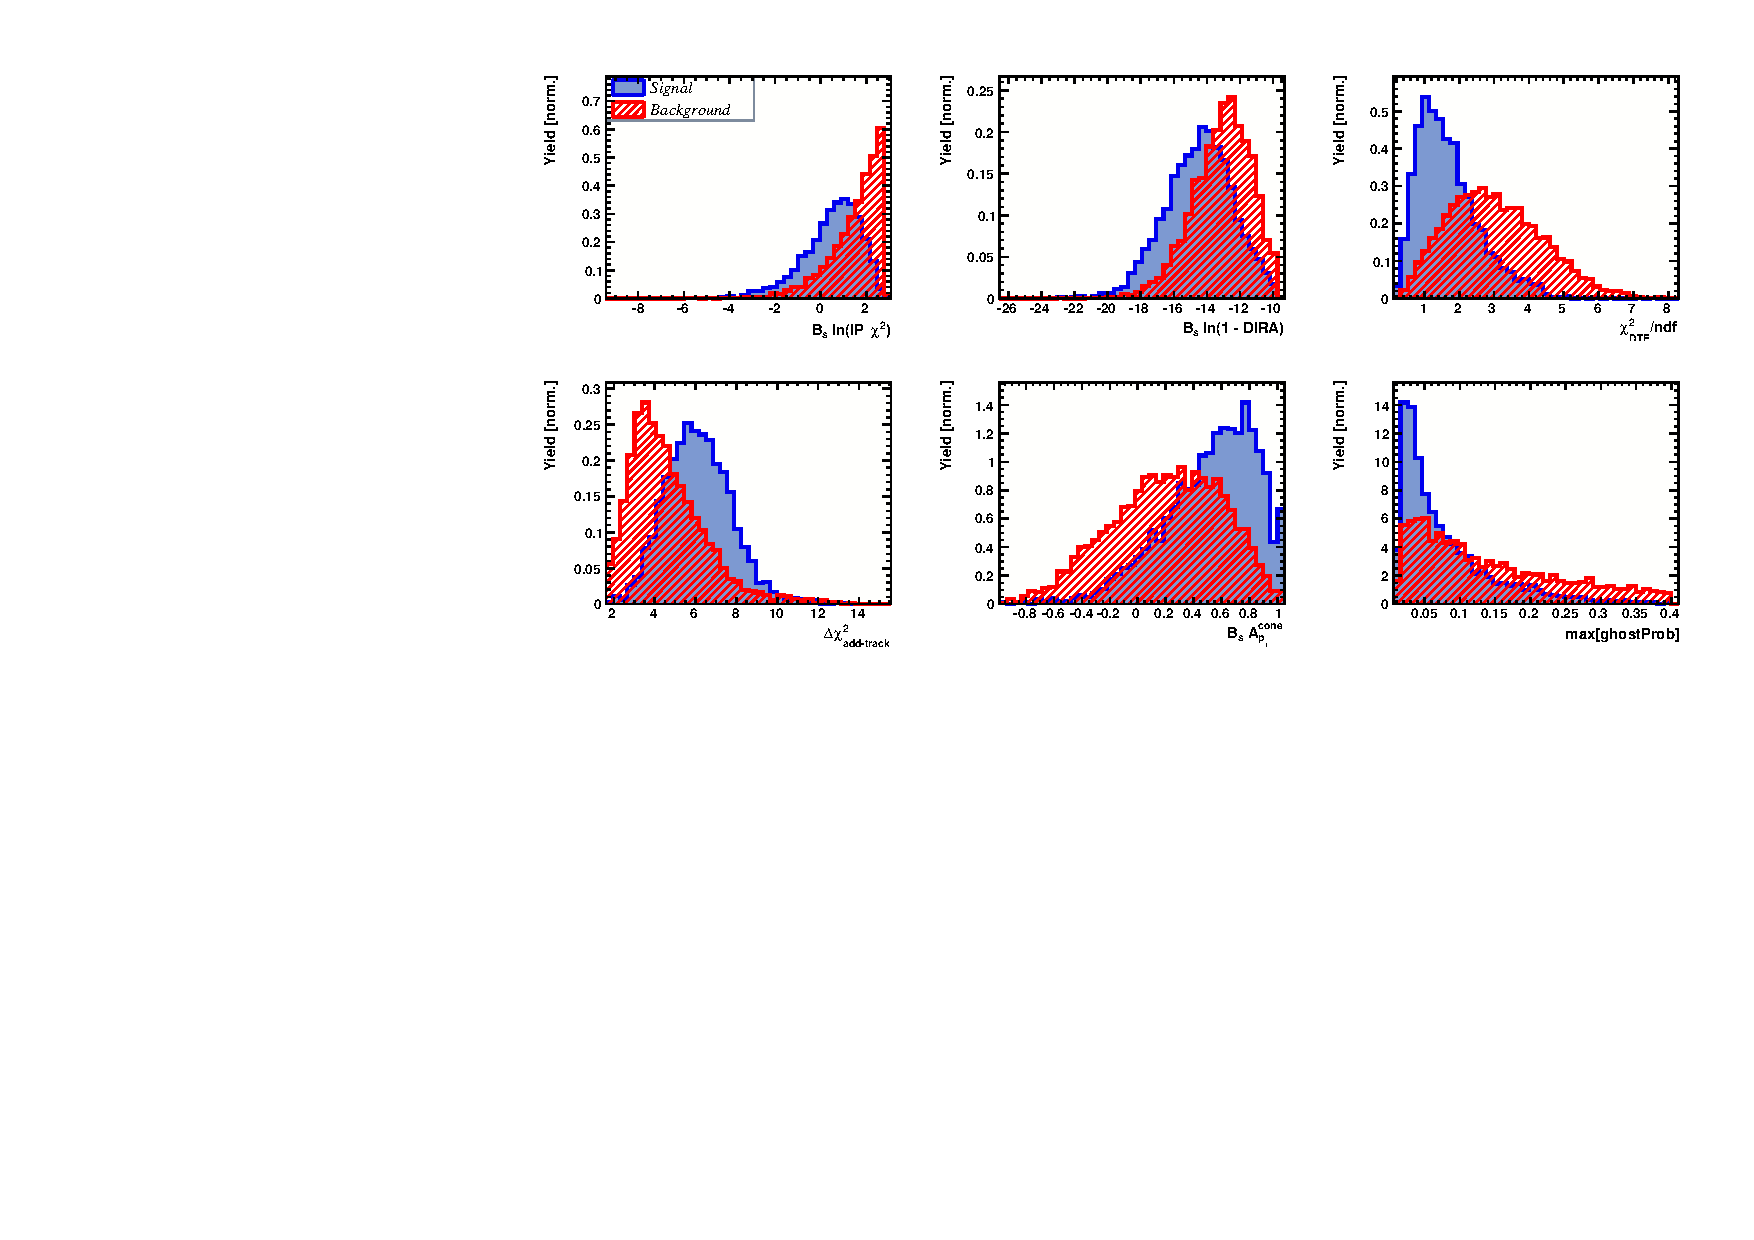
\includegraphics[height=5cm,width=0.9\textwidth]{figs/TMVA/BDTG_Data_run1_t0_all/variables_id_c1.pdf}
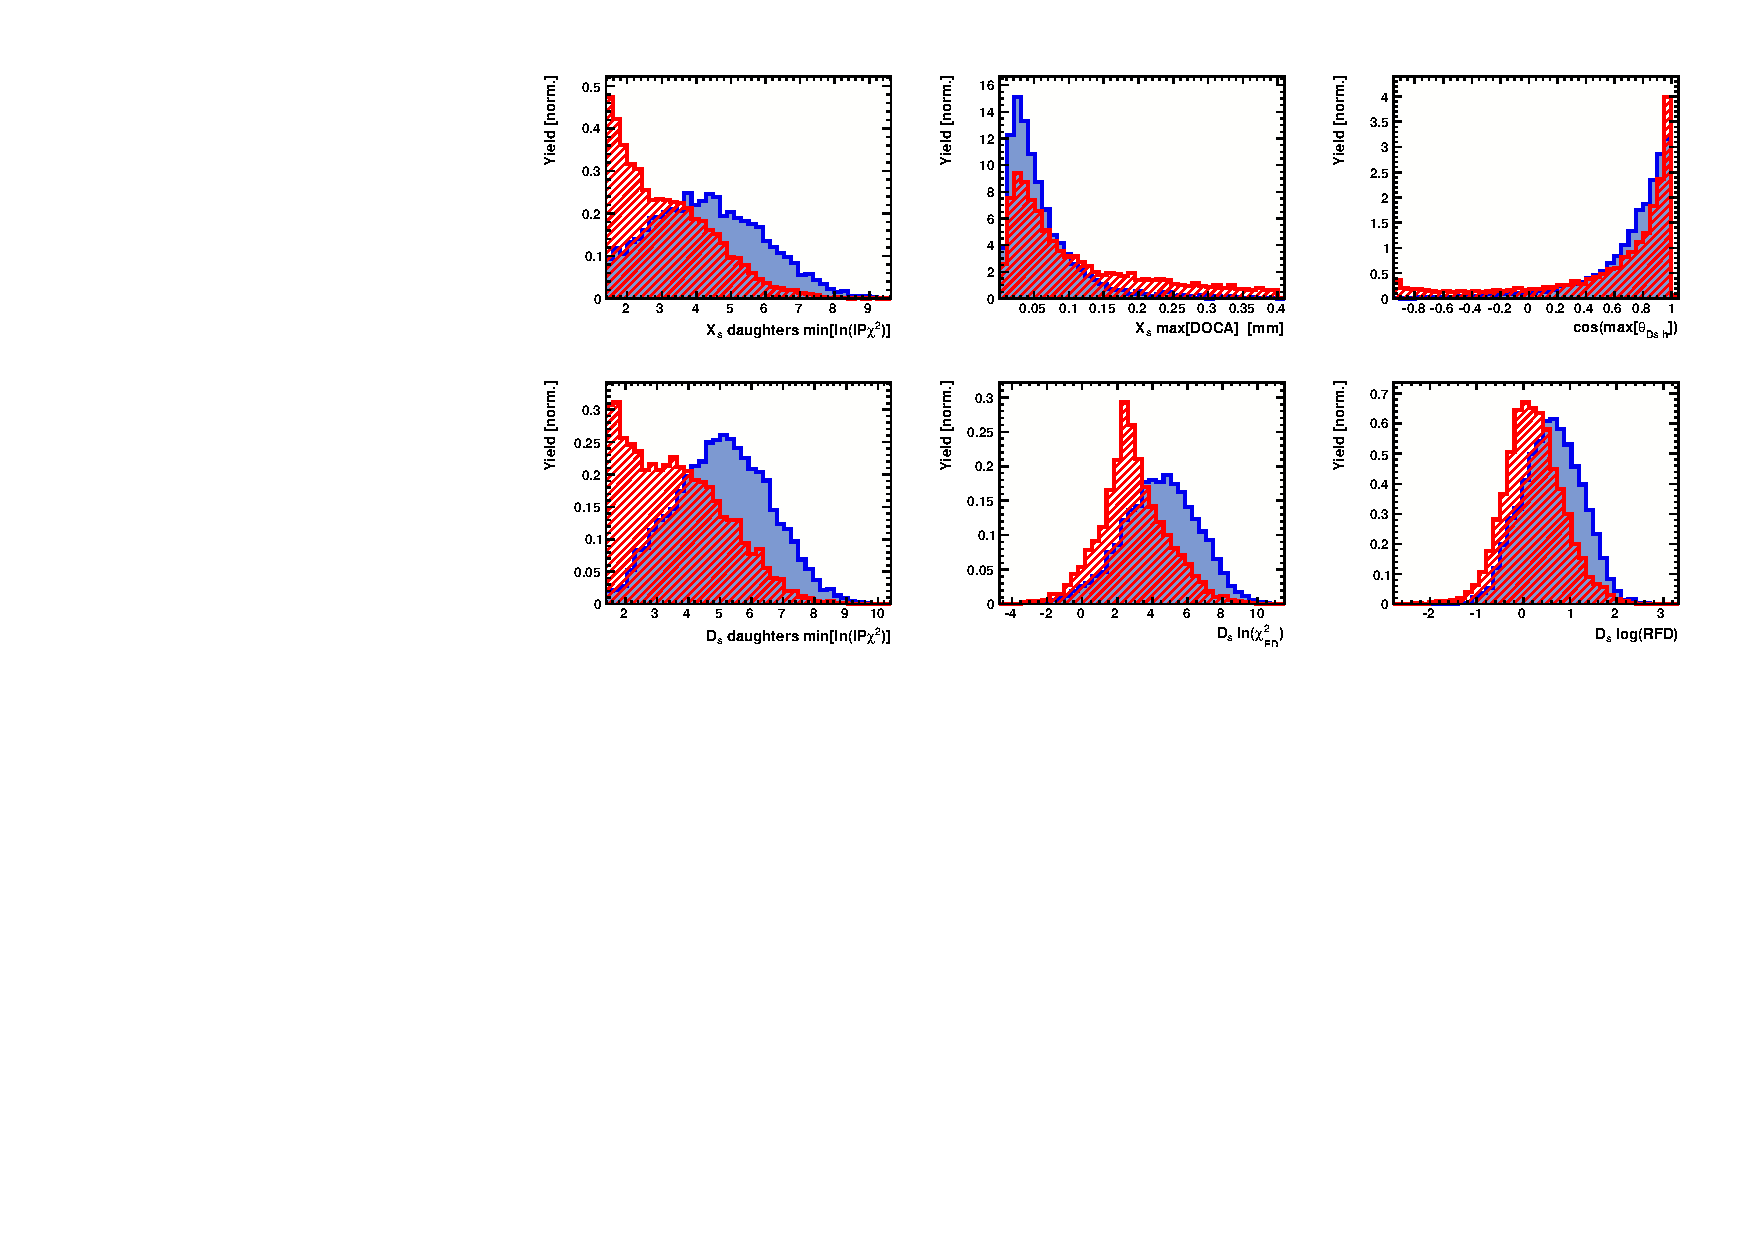
\includegraphics[height=5cm,width=0.9\textwidth]{figs/TMVA/BDTG_Data_run1_t0_all/variables_id_c2.pdf}
\caption{Variables used to train the BDTG for category [Run-I,\textsf{L0-TOS}].}
\label{fig:}
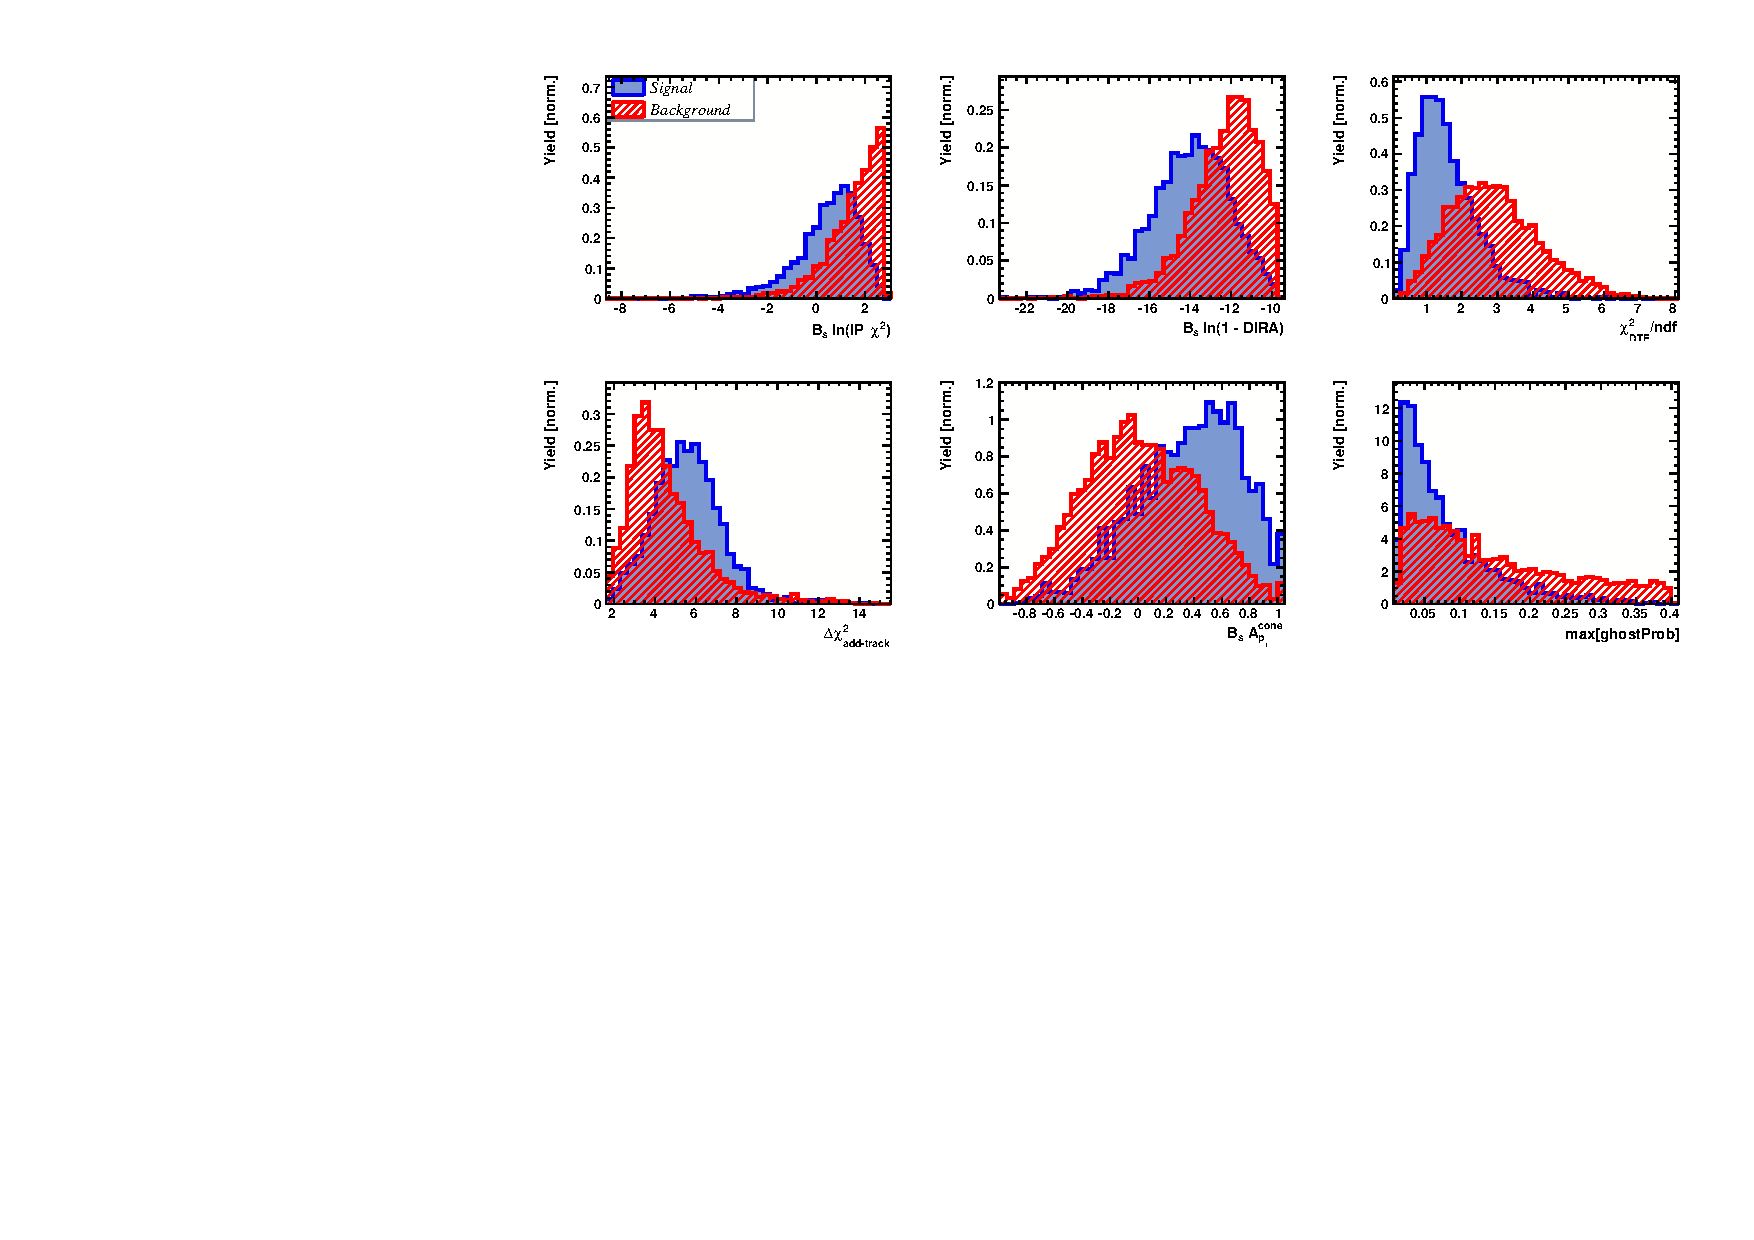
\includegraphics[height=5cm,width=0.9\textwidth]{figs/TMVA/BDTG_Data_run1_t1_all/variables_id_c1.pdf}
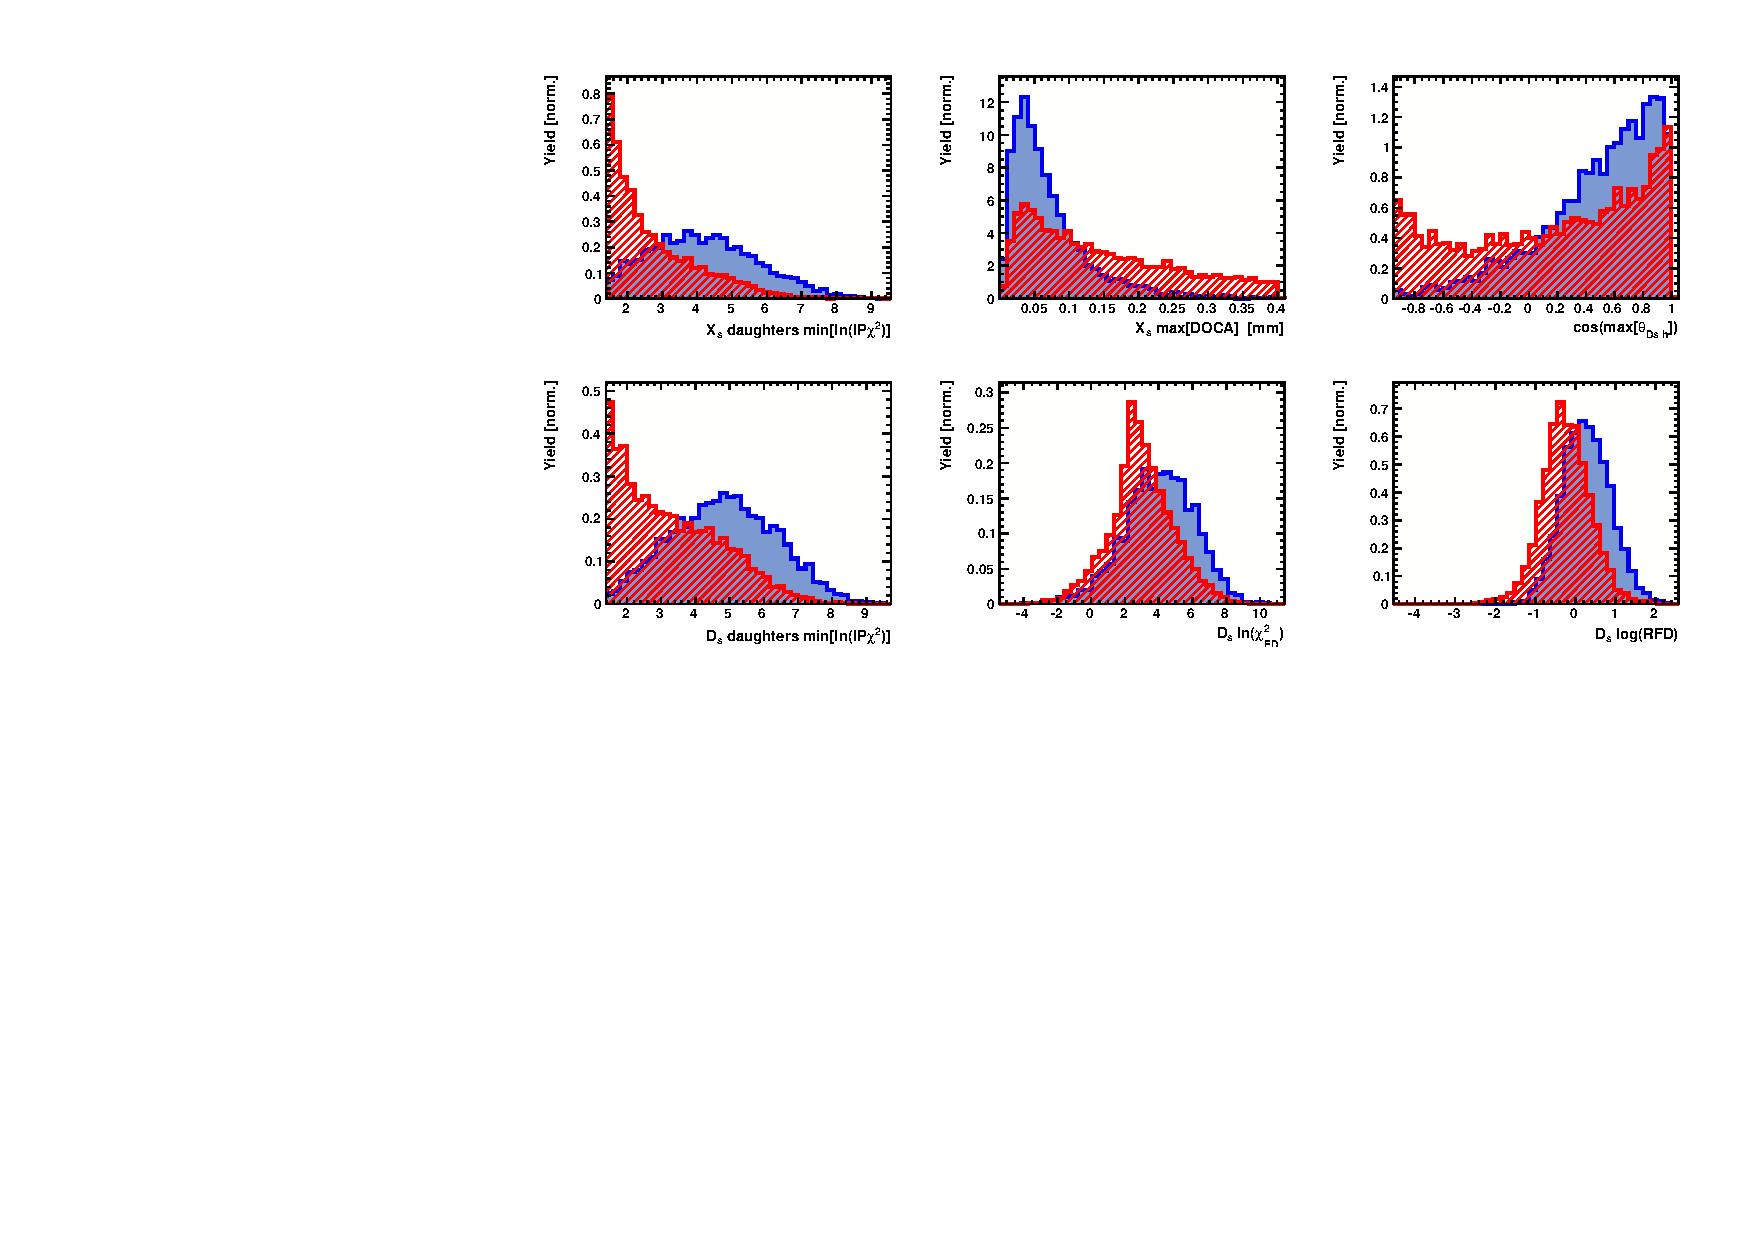
\includegraphics[height=5cm,width=0.9\textwidth]{figs/TMVA/BDTG_Data_run1_t1_all/variables_id_c2.pdf}
\caption{Variables used to train the BDTG for category [Run-I,\textsf{L0-TIS}].}
\label{fig:}
\end{figure}

\begin{figure}[h]
\centering
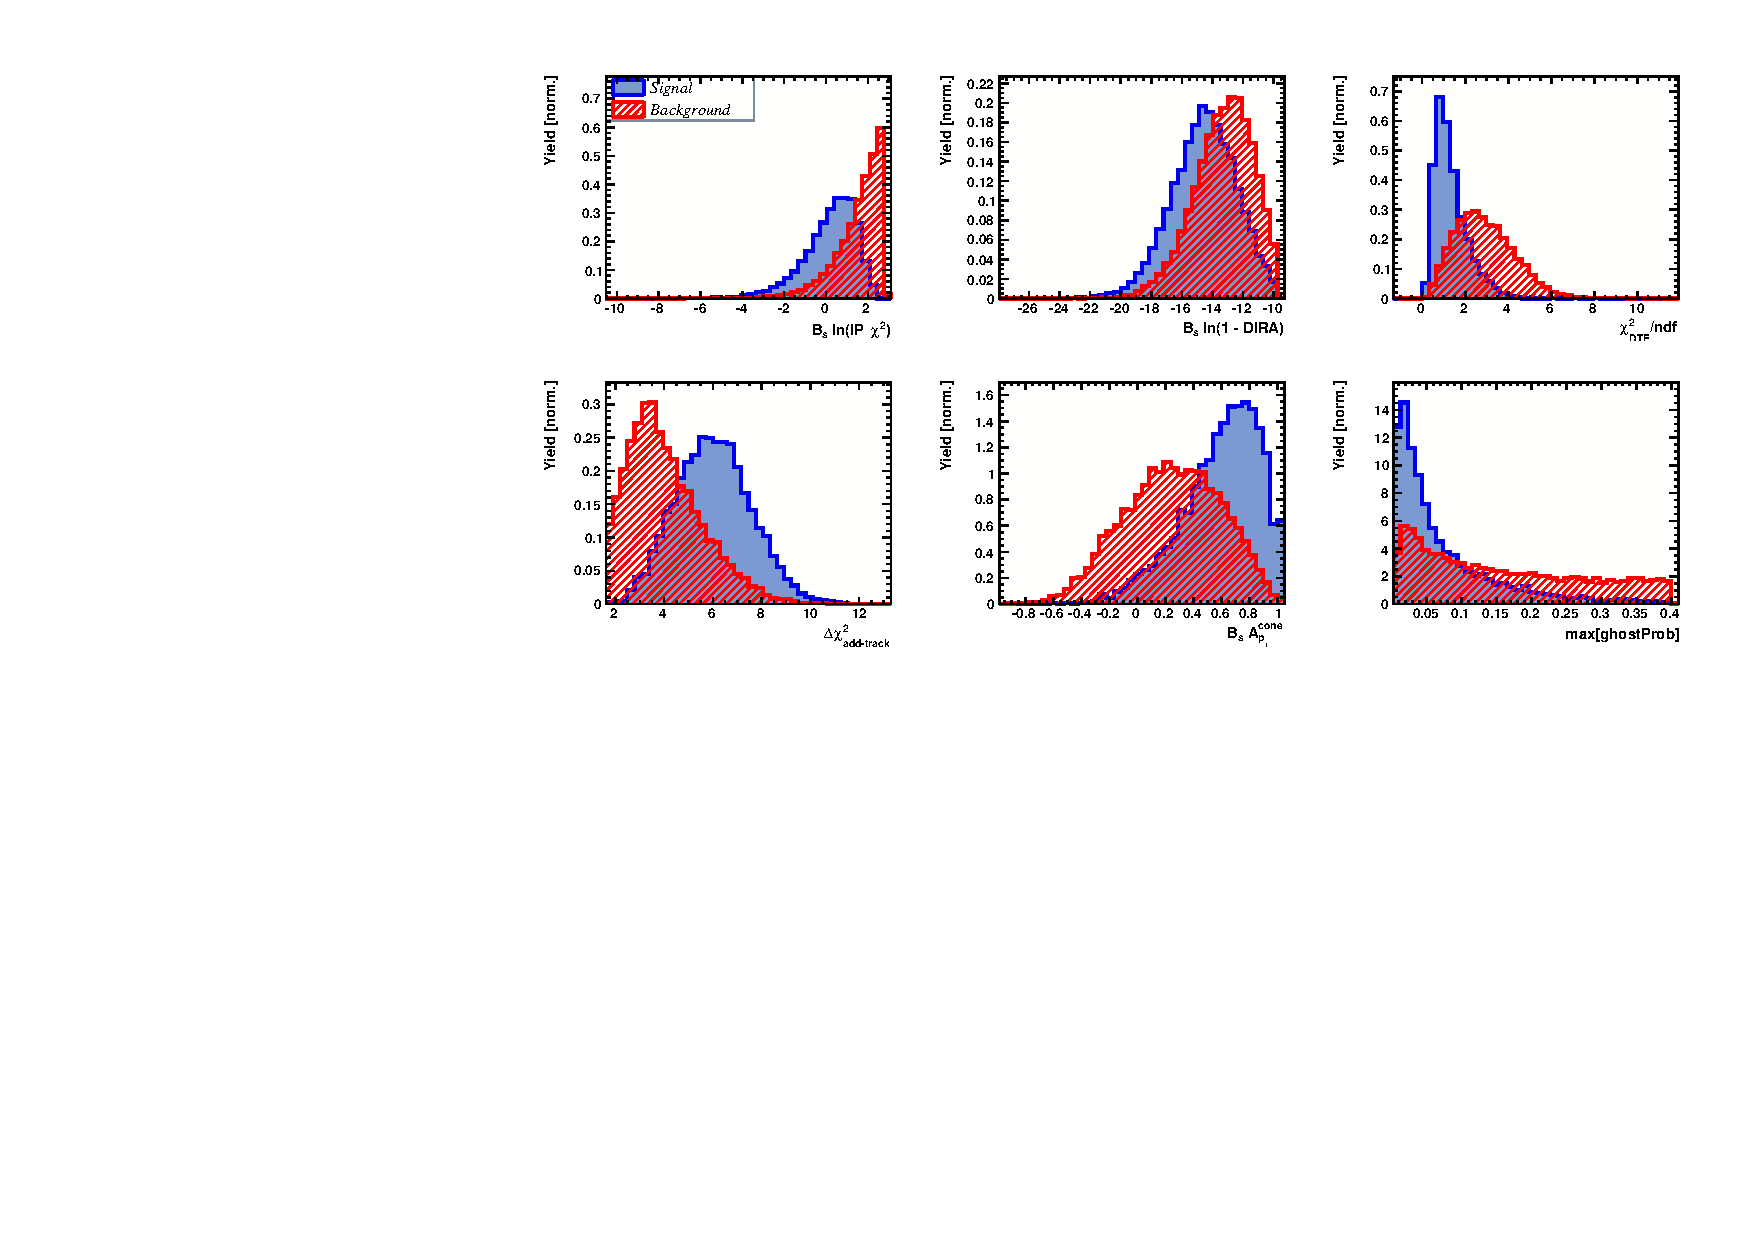
\includegraphics[height=5cm,width=0.9\textwidth]{figs/TMVA/BDTG_Data_run2_t0_all/variables_id_c1.pdf}
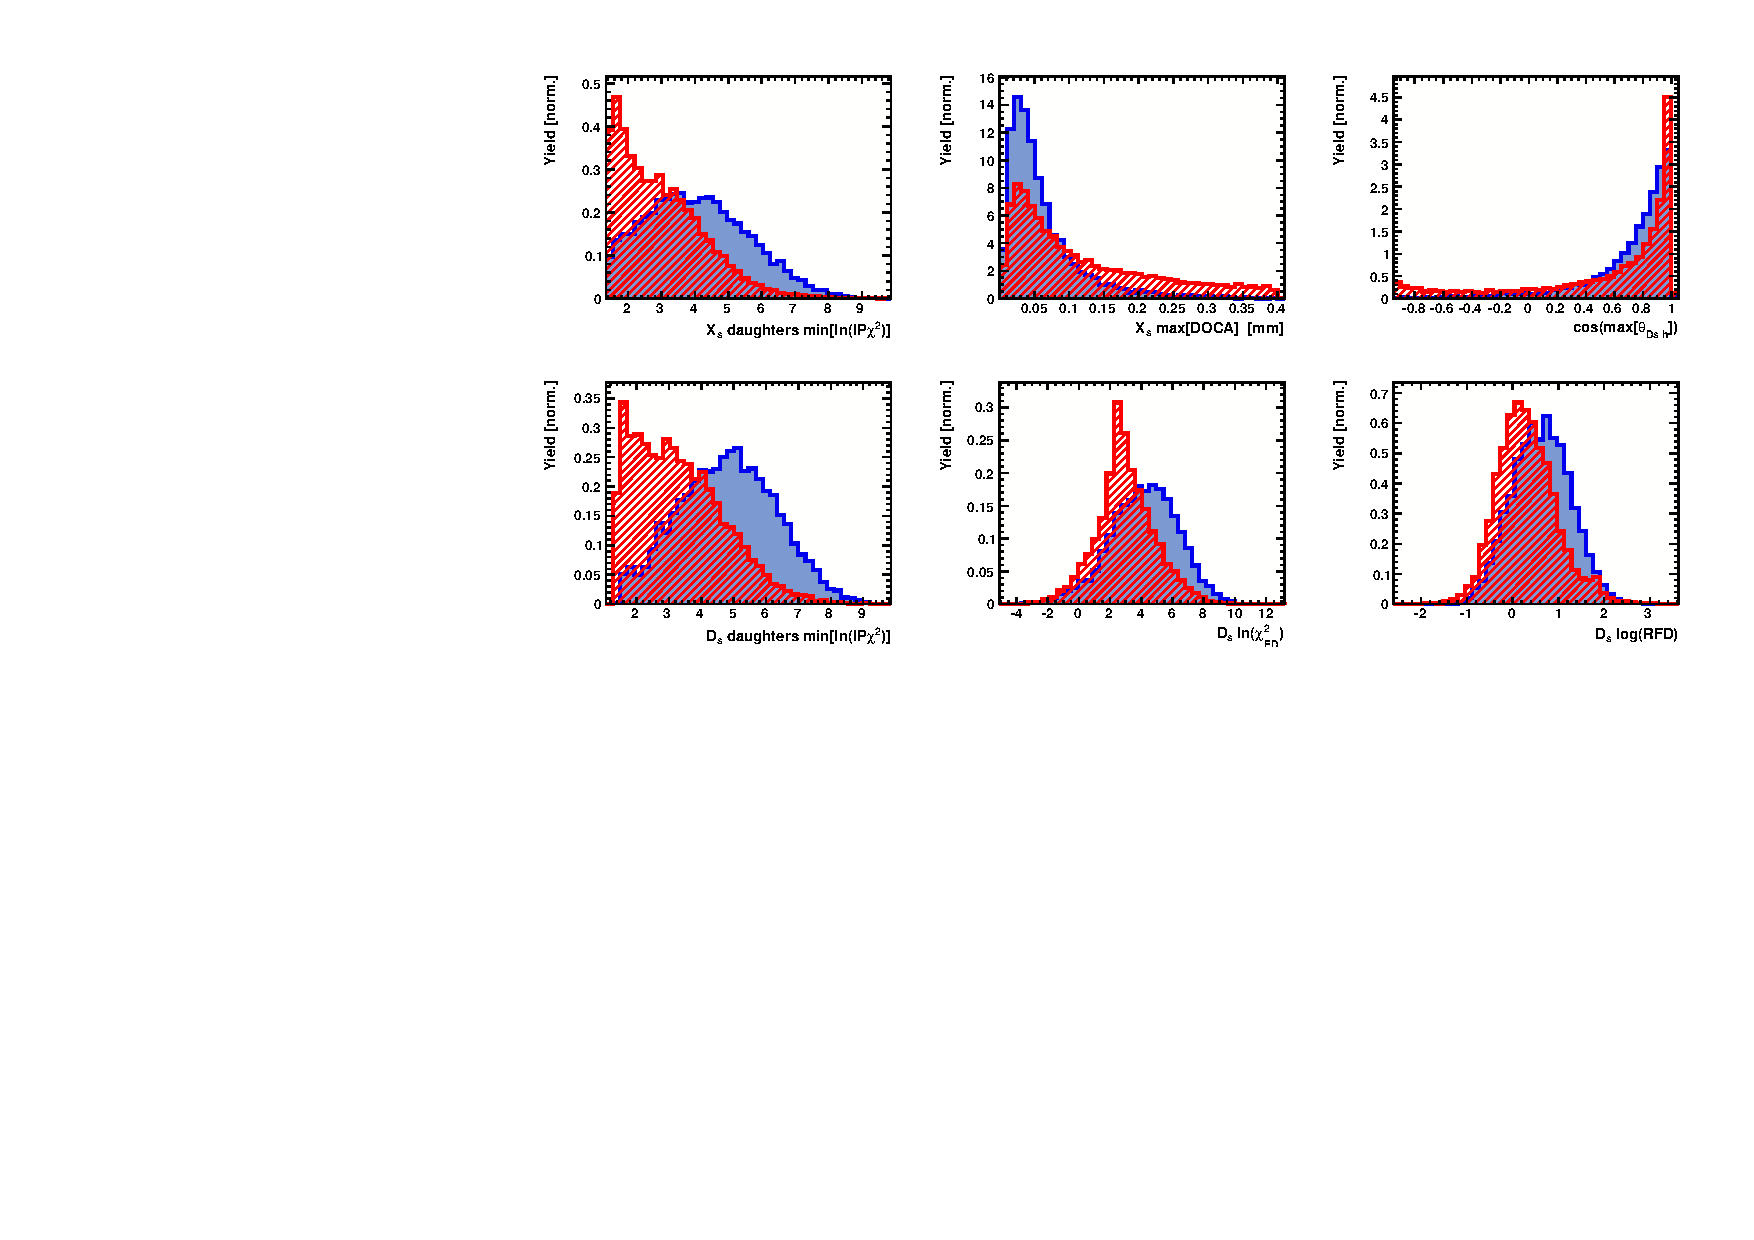
\includegraphics[height=5cm,width=0.9\textwidth]{figs/TMVA/BDTG_Data_run2_t0_all/variables_id_c2.pdf}
\caption{Variables used to train the BDTG for category [Run-II,\textsf{L0-TOS}].}
\label{fig:}
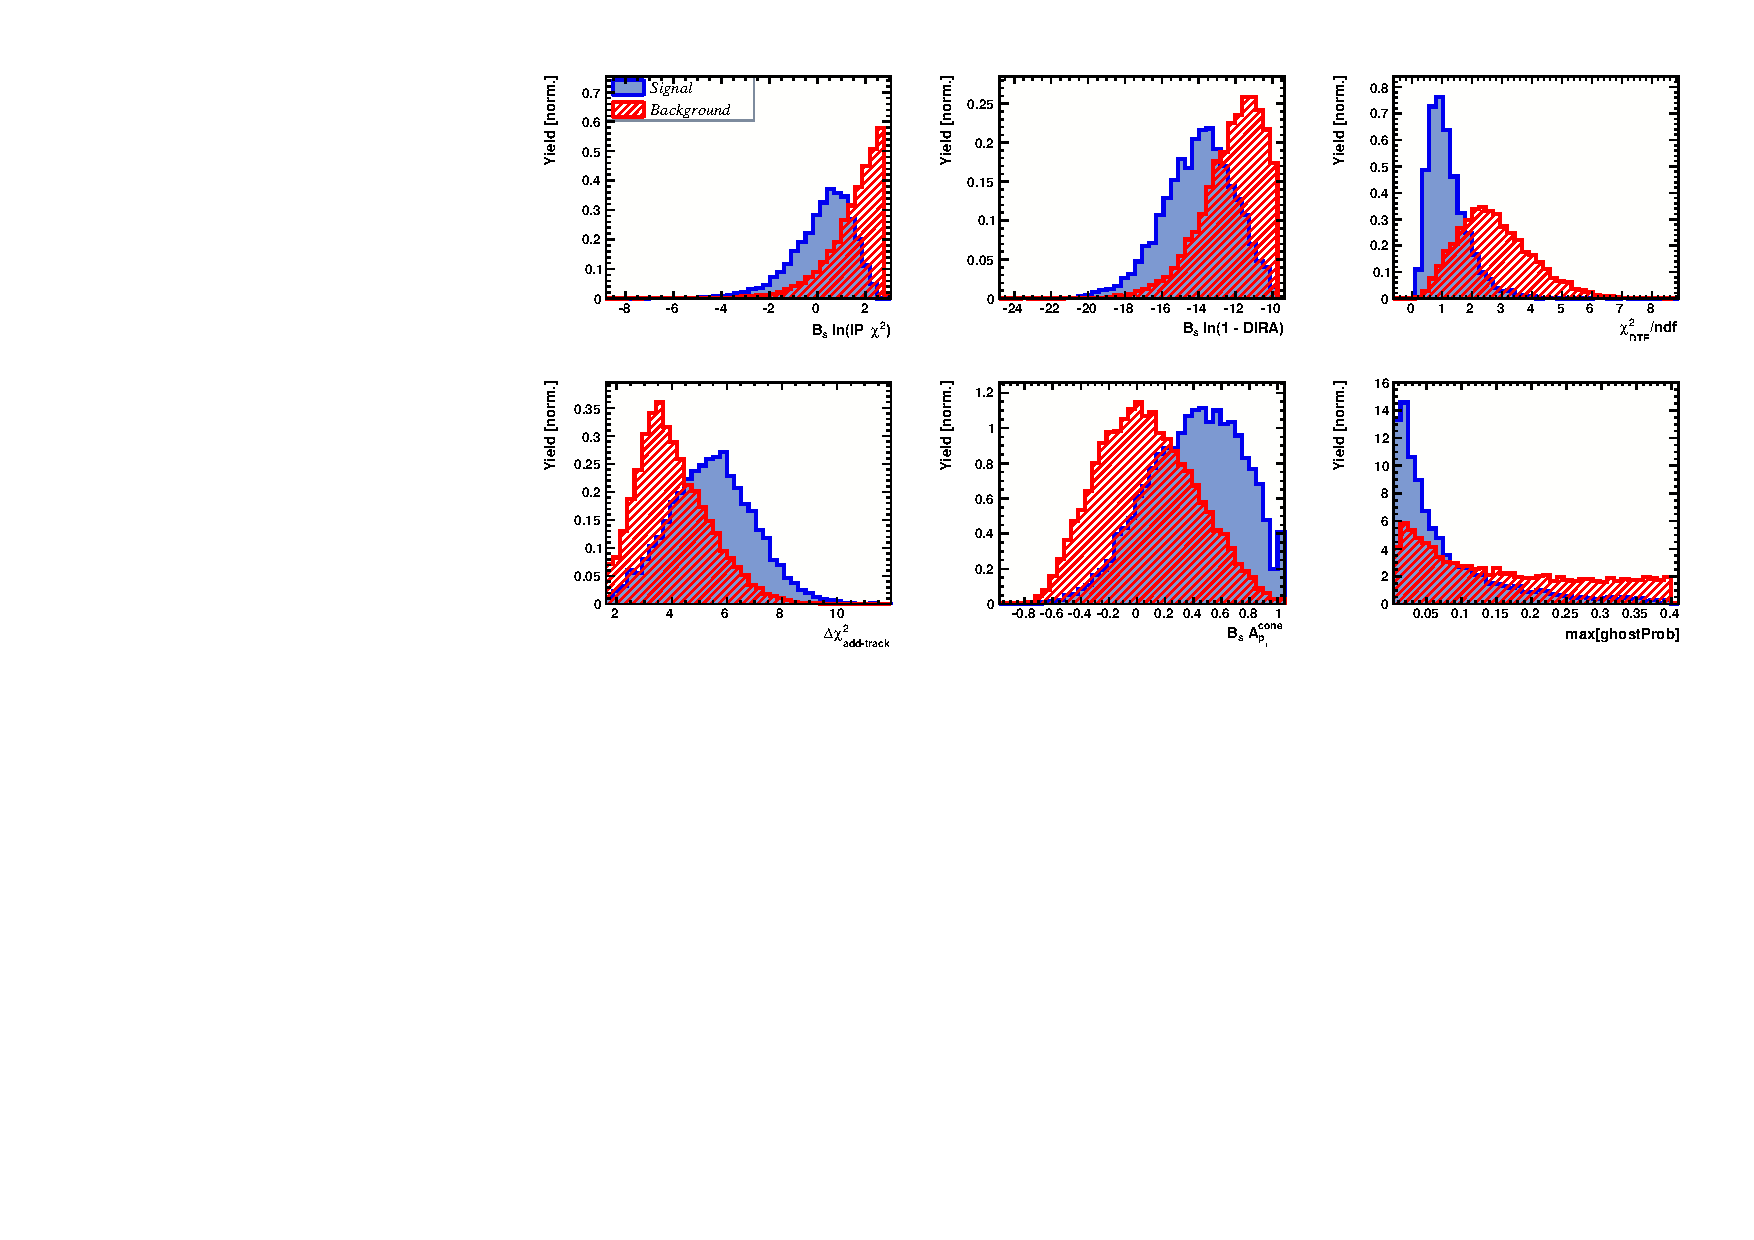
\includegraphics[height=5cm,width=0.9\textwidth]{figs/TMVA/BDTG_Data_run2_t1_all/variables_id_c1.pdf}
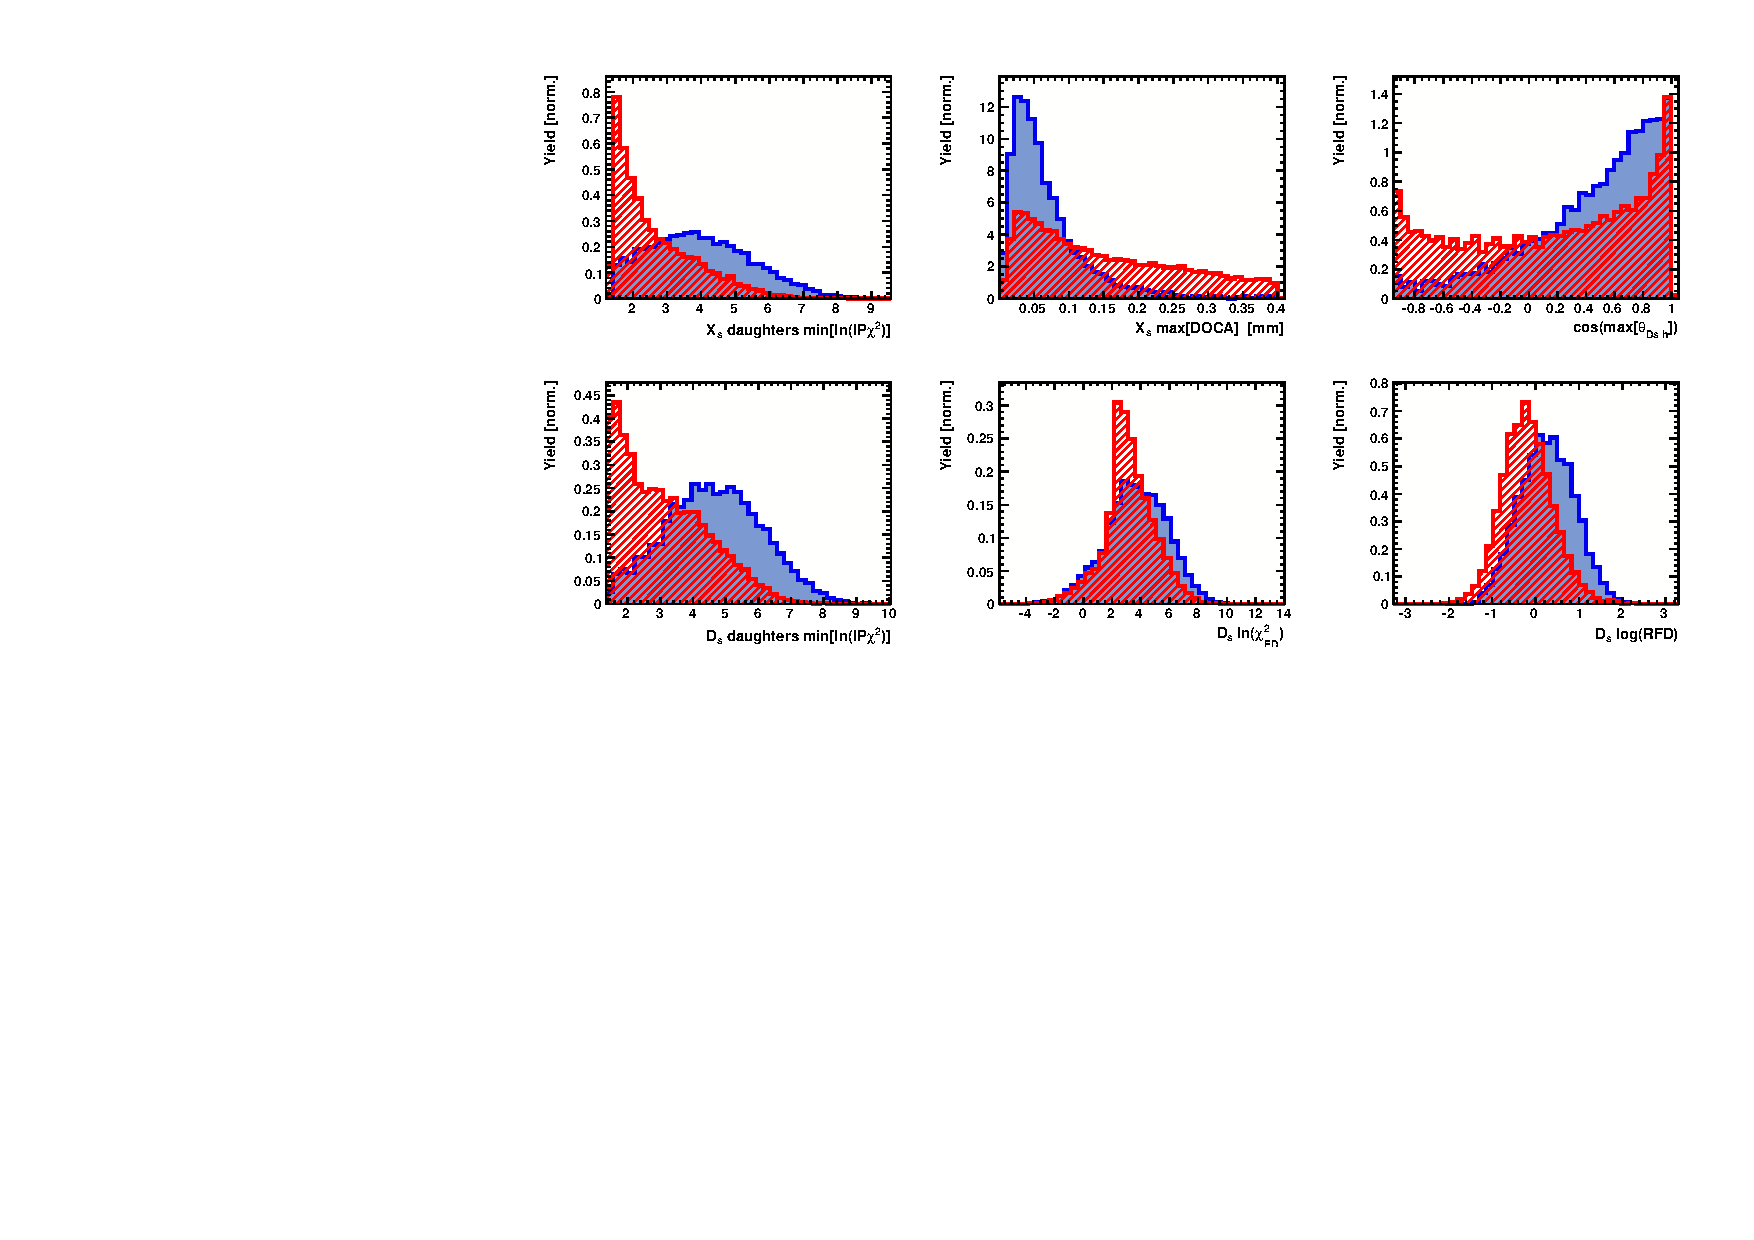
\includegraphics[height=5cm,width=0.9\textwidth]{figs/TMVA/BDTG_Data_run2_t1_all/variables_id_c2.pdf}
\caption{Variables used to train the BDTG for category [Run-II,\textsf{L0-TIS}].}
\label{fig:}
\end{figure}

\begin{figure}[h]
\centering
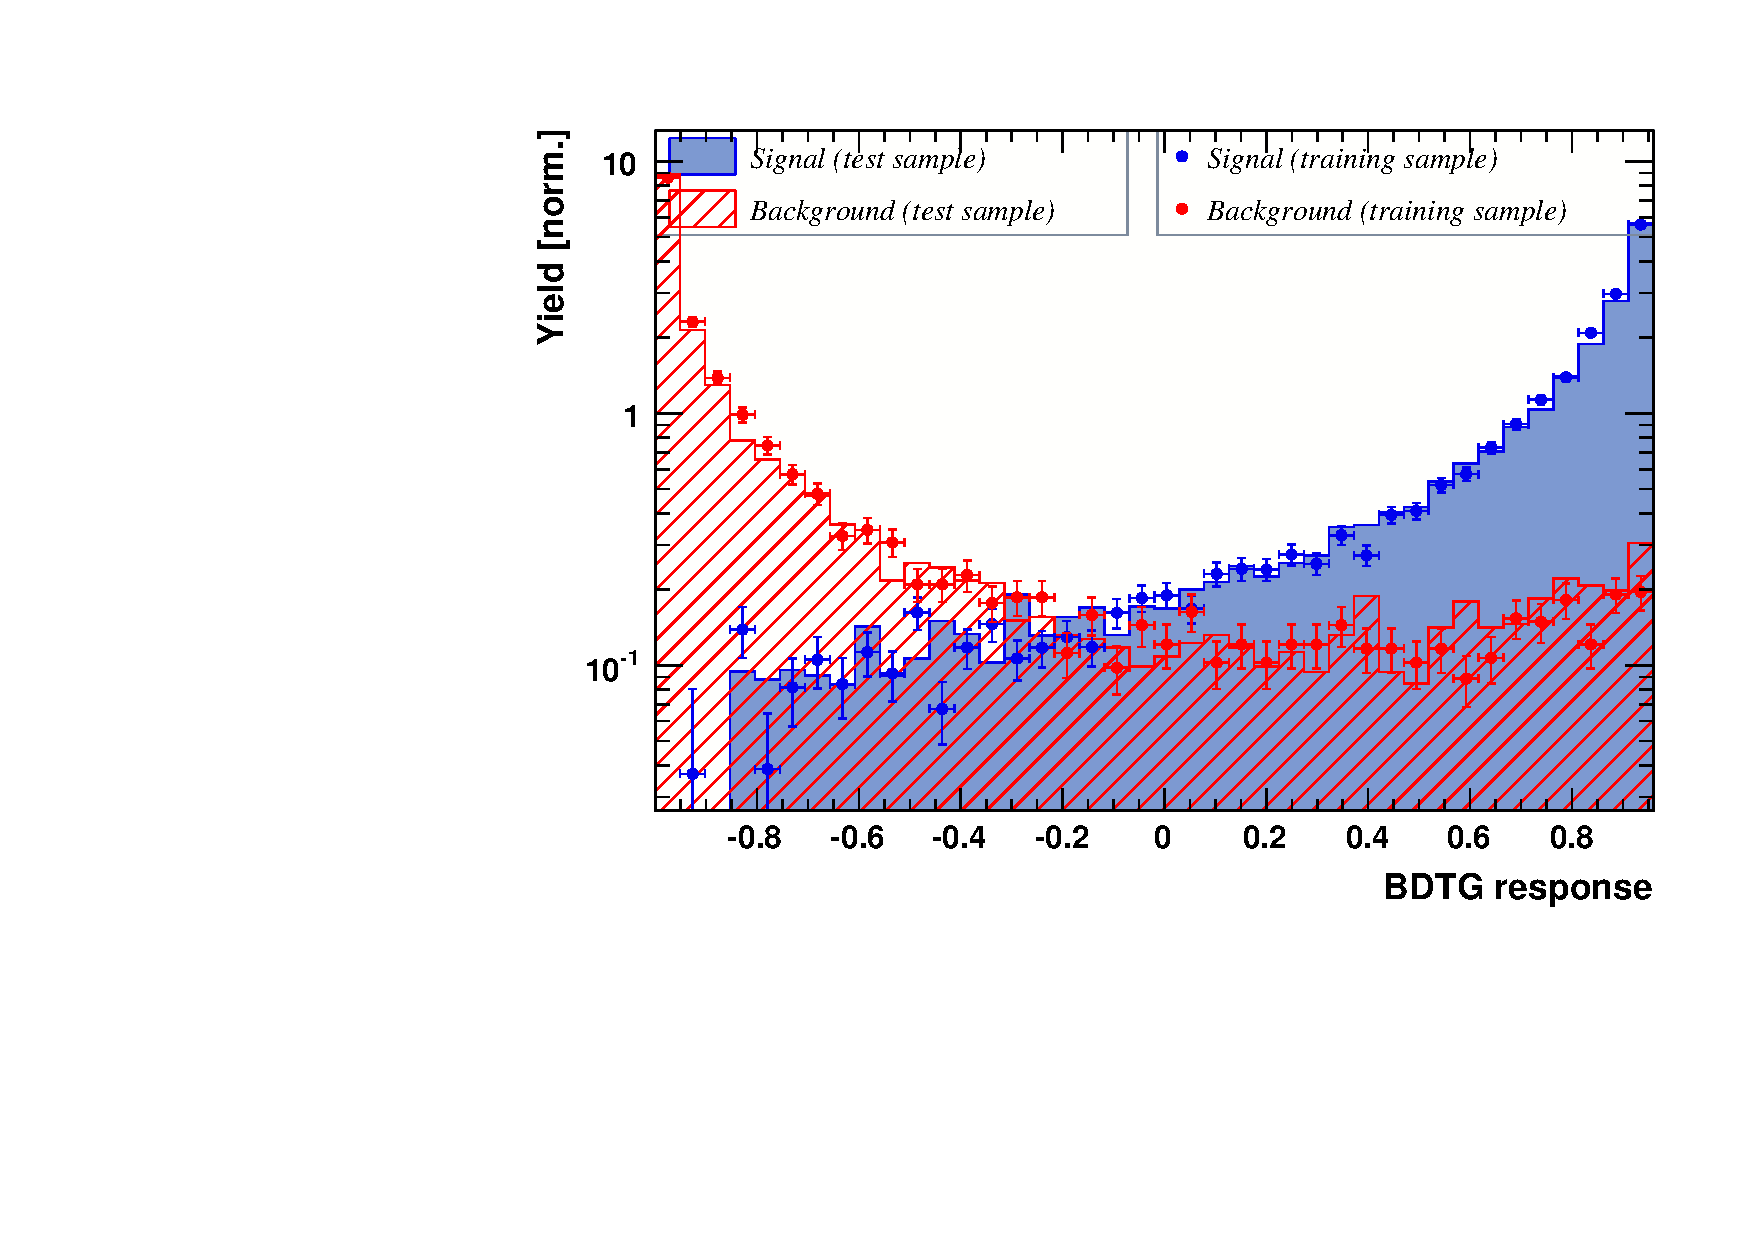
\includegraphics[height=!,width=0.4\textwidth]{figs/TMVA/BDTG_Data_run1_t0_even/overtrain_BDTG.pdf}
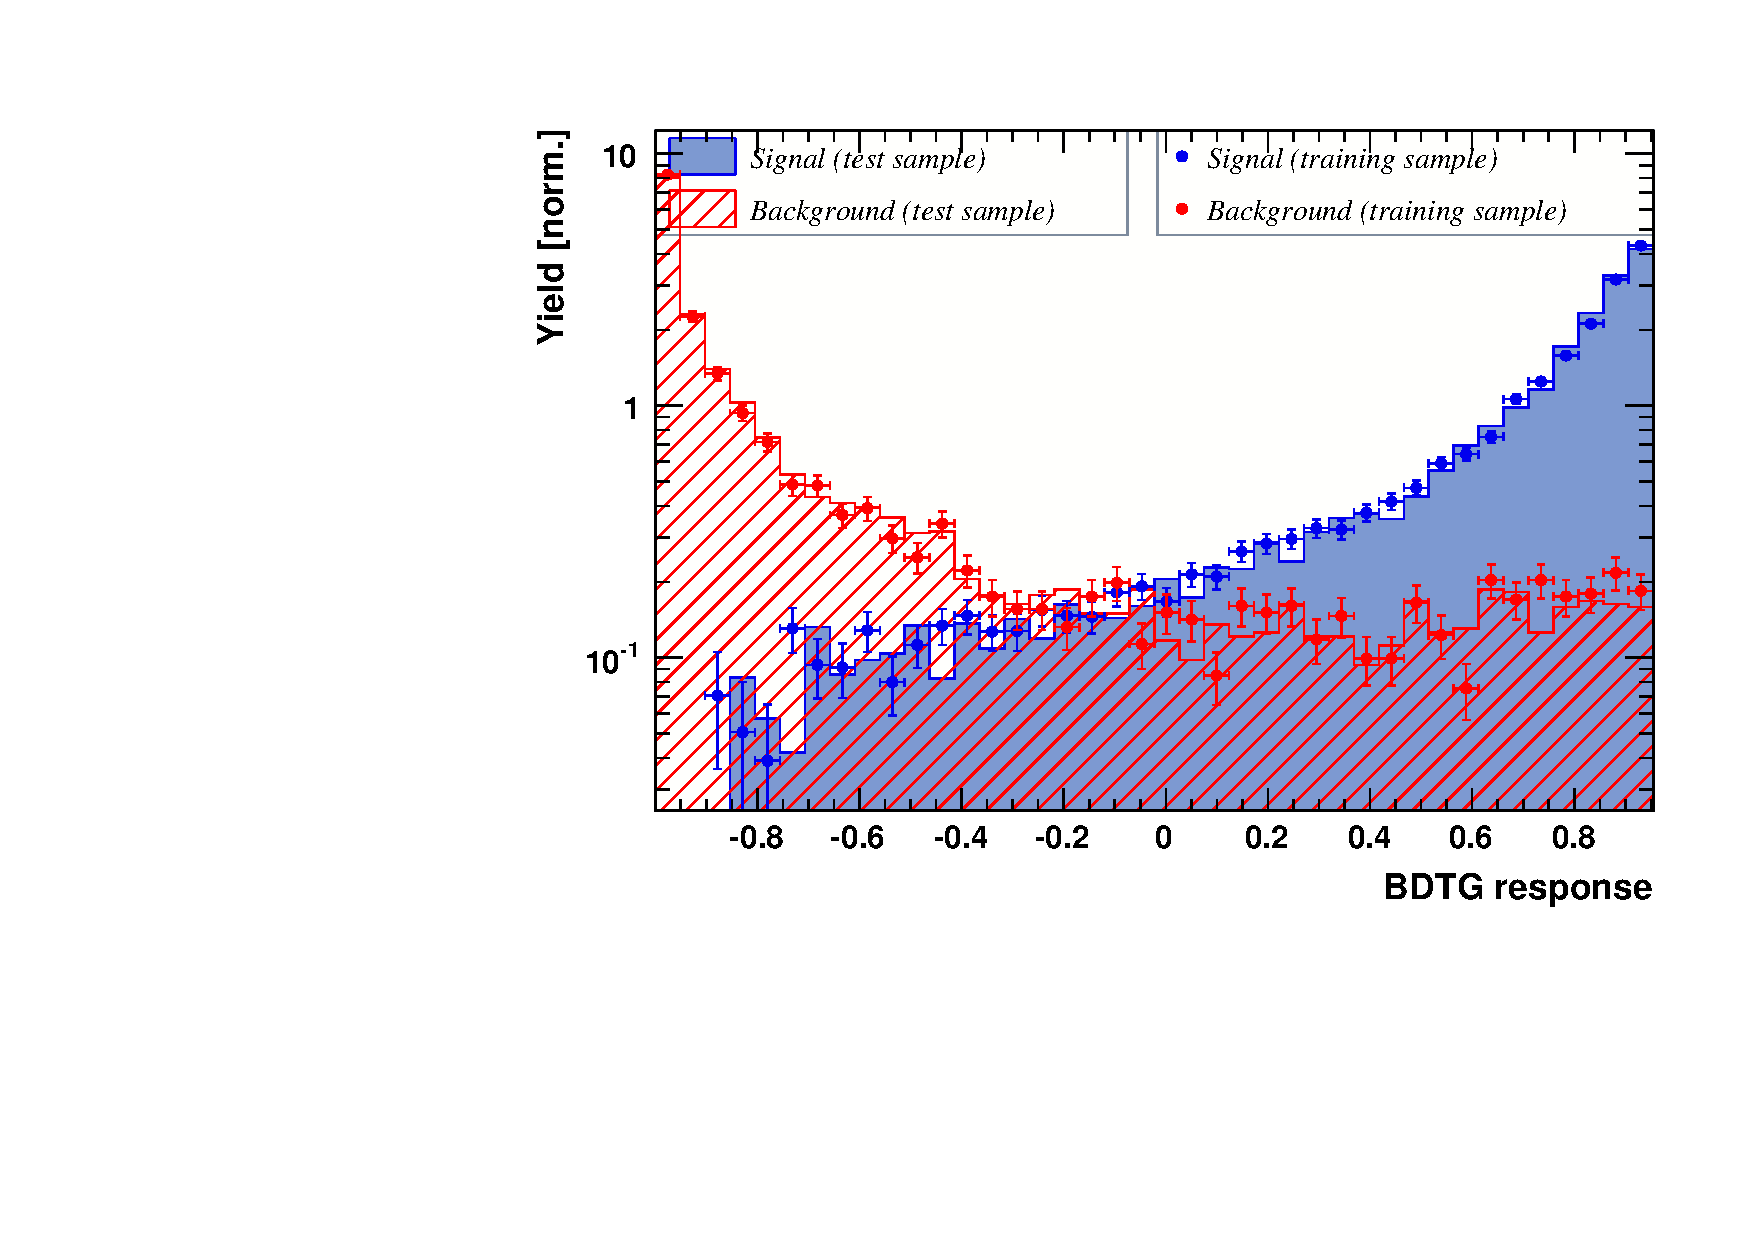
\includegraphics[height=!,width=0.4\textwidth]{figs/TMVA/BDTG_Data_run1_t0_odd/overtrain_BDTG.pdf}
\caption{Response of the classifier trained on the even and tested on the odd sample (left) and trained on the odd and tested on the even sample (right) for category [Run-I,\textsf{L0-TOS}].}

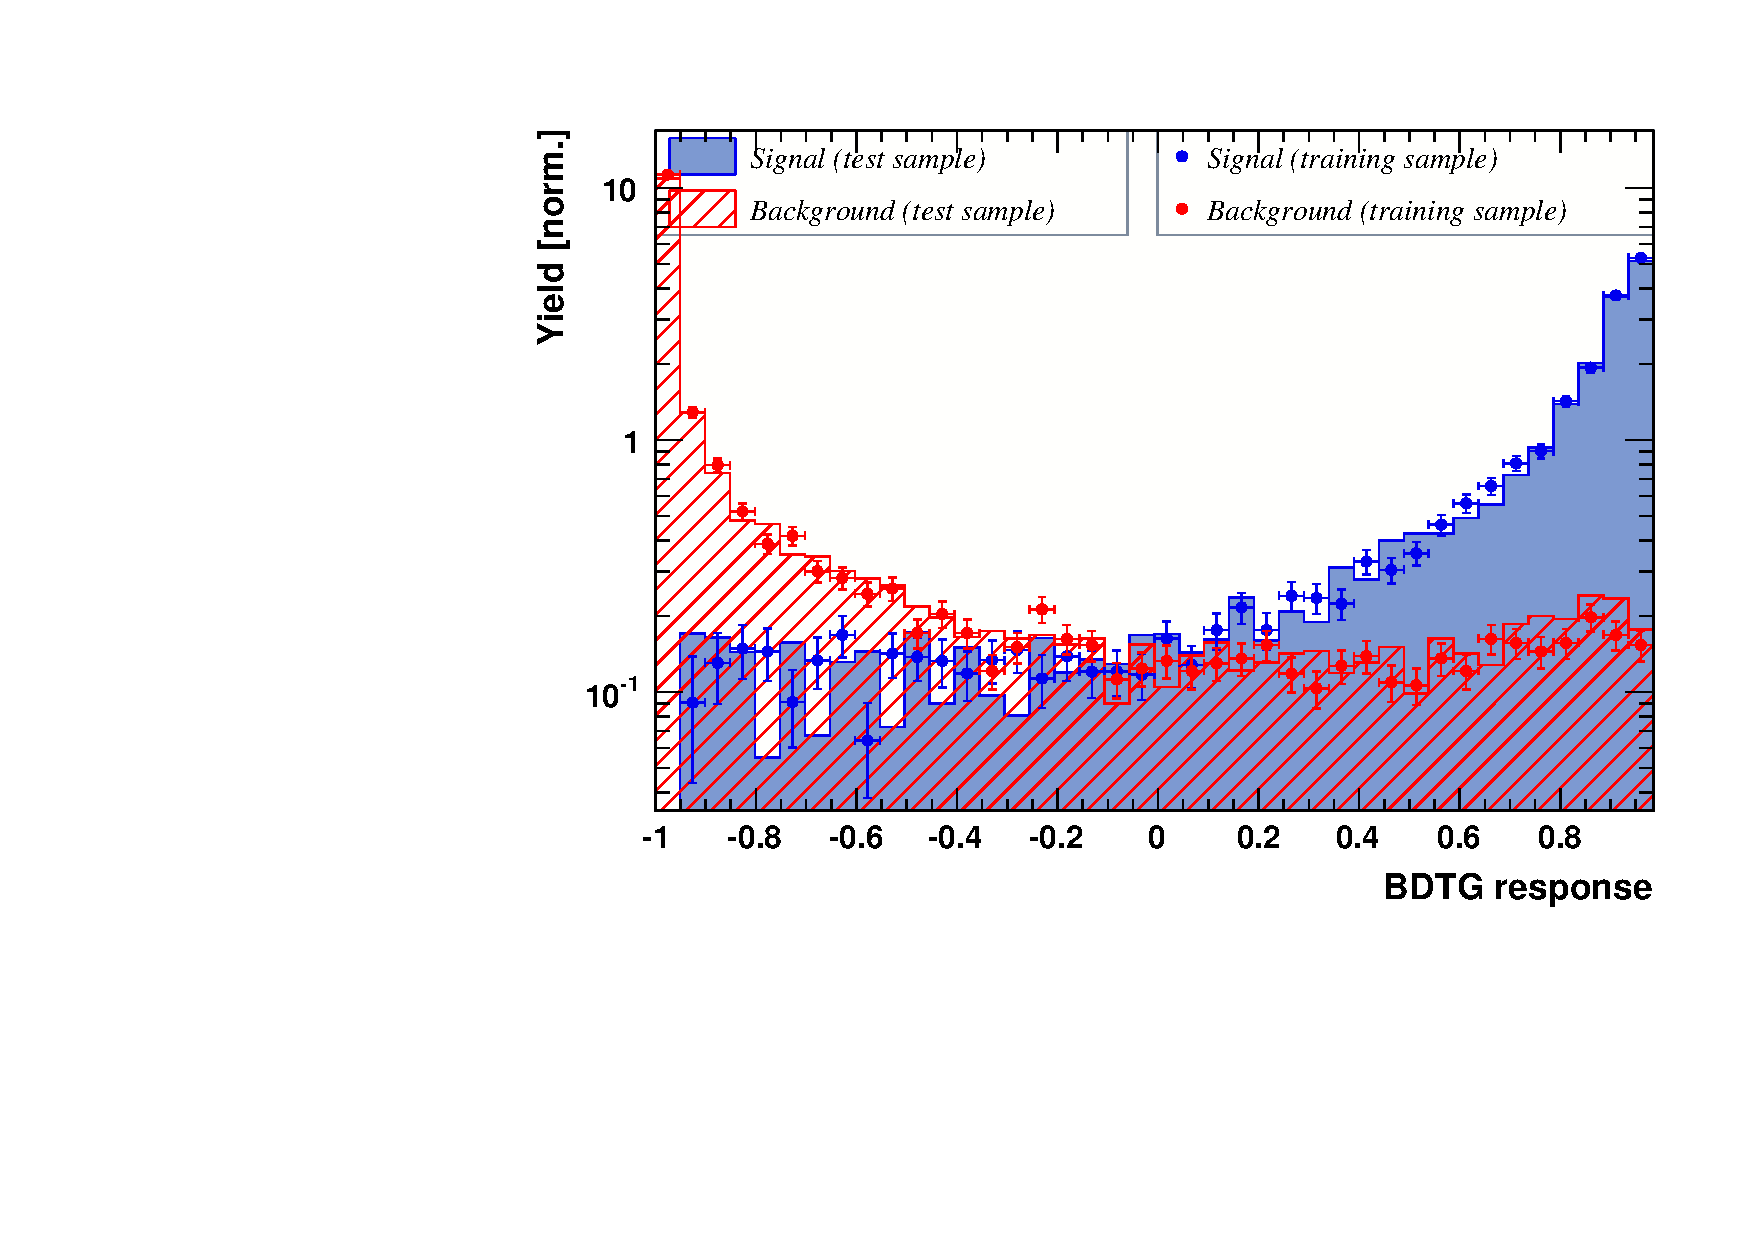
\includegraphics[height=!,width=0.4\textwidth]{figs/TMVA/BDTG_Data_run1_t1_even/overtrain_BDTG.pdf}
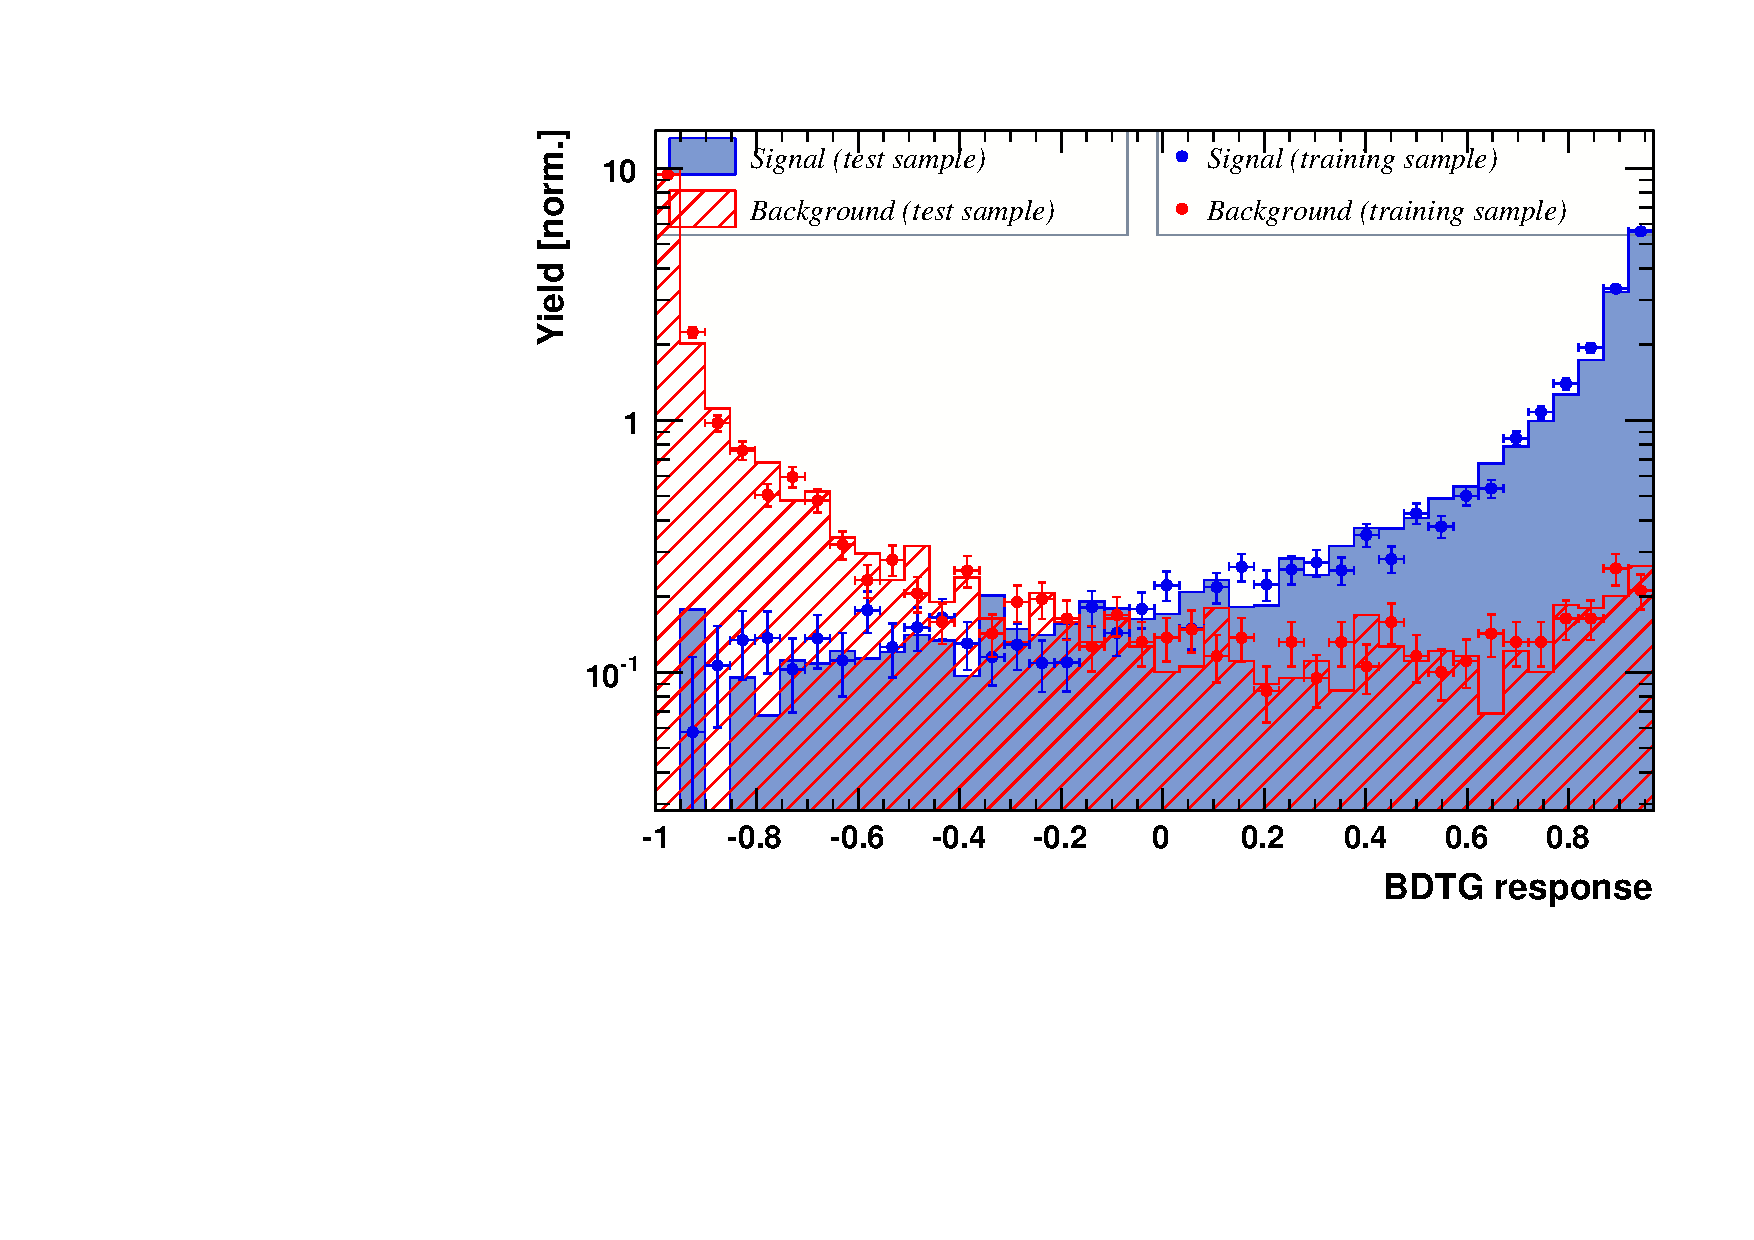
\includegraphics[height=!,width=0.4\textwidth]{figs/TMVA/BDTG_Data_run1_t1_odd/overtrain_BDTG.pdf}
\caption{Response of the classifier trained on the even and tested on the odd sample (left) and trained on the odd and tested on the even sample (right) for category [Run-I,\textsf{L0-TIS}].}

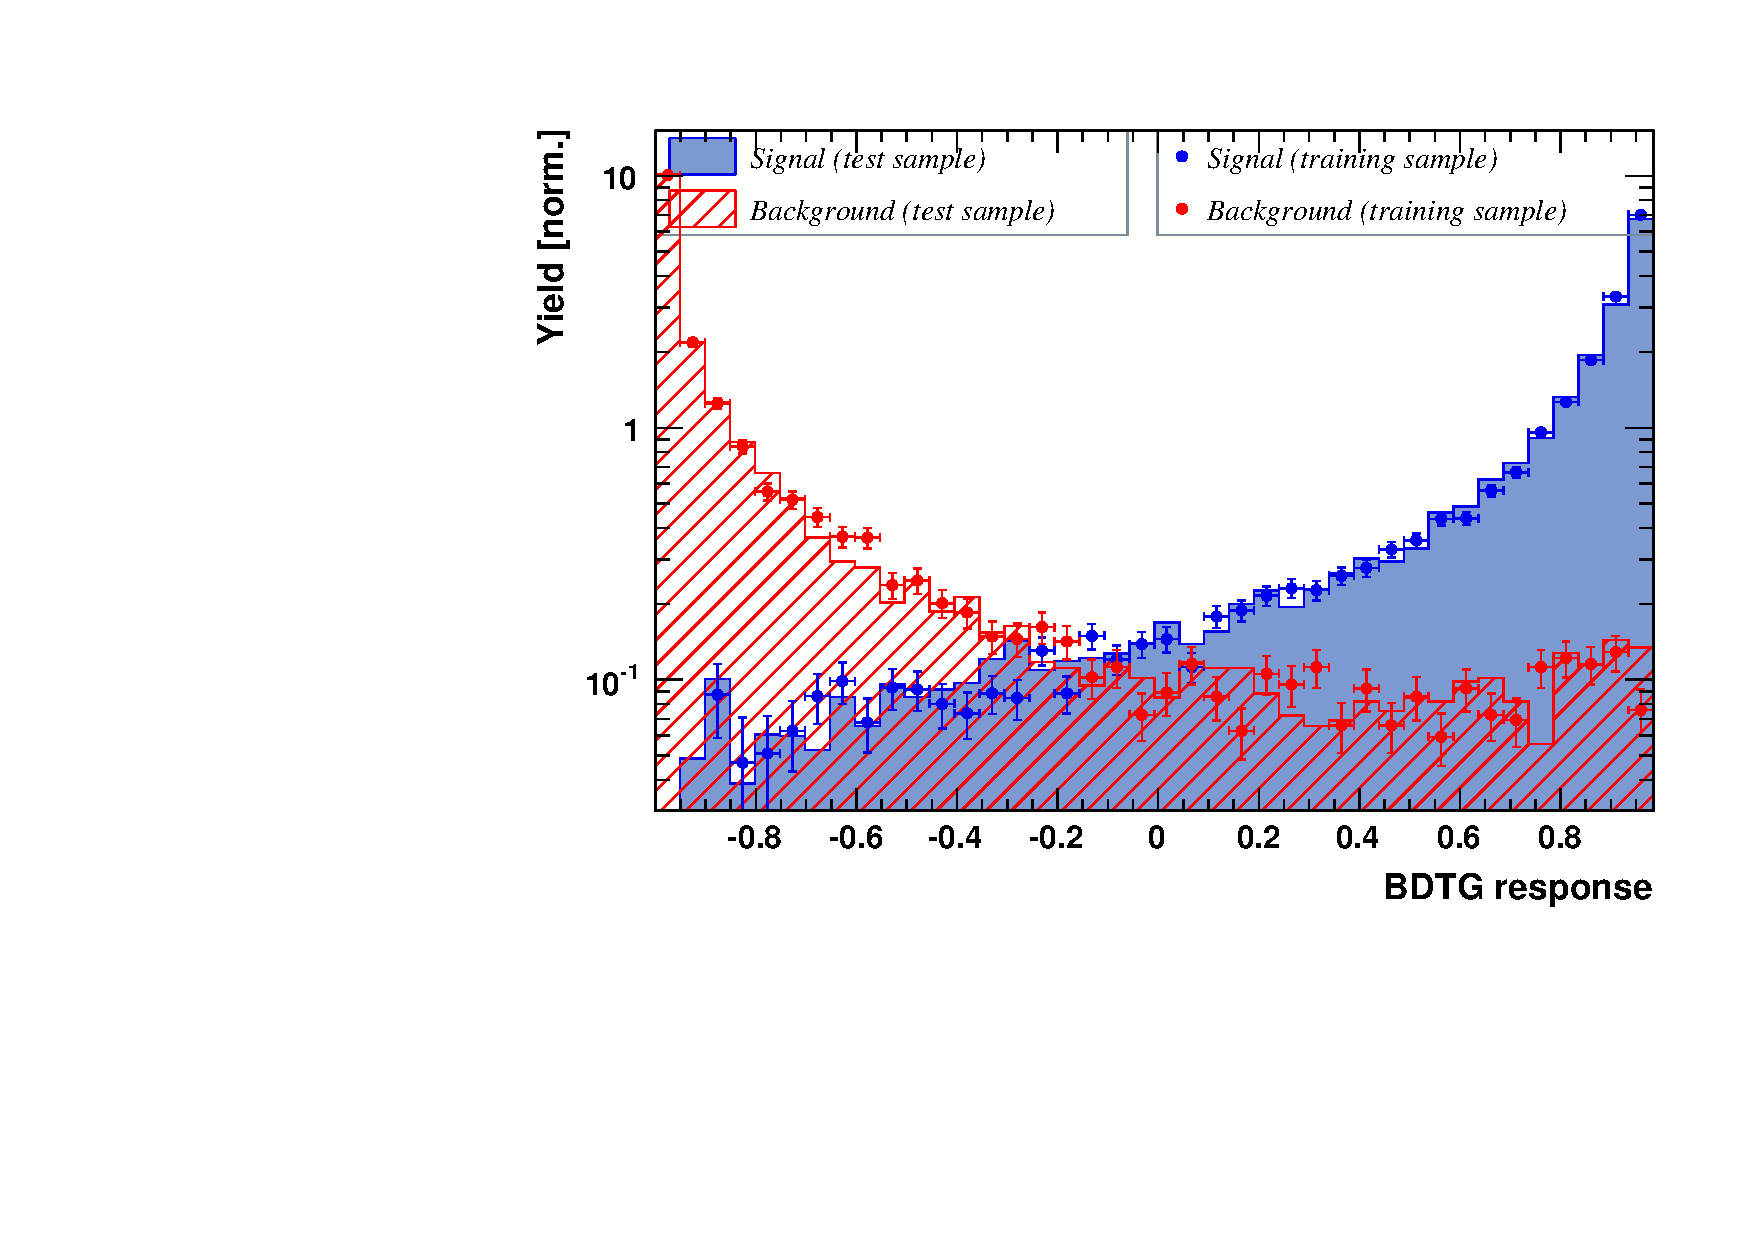
\includegraphics[height=!,width=0.4\textwidth]{figs/TMVA/BDTG_Data_run2_t0_even/overtrain_BDTG.pdf}
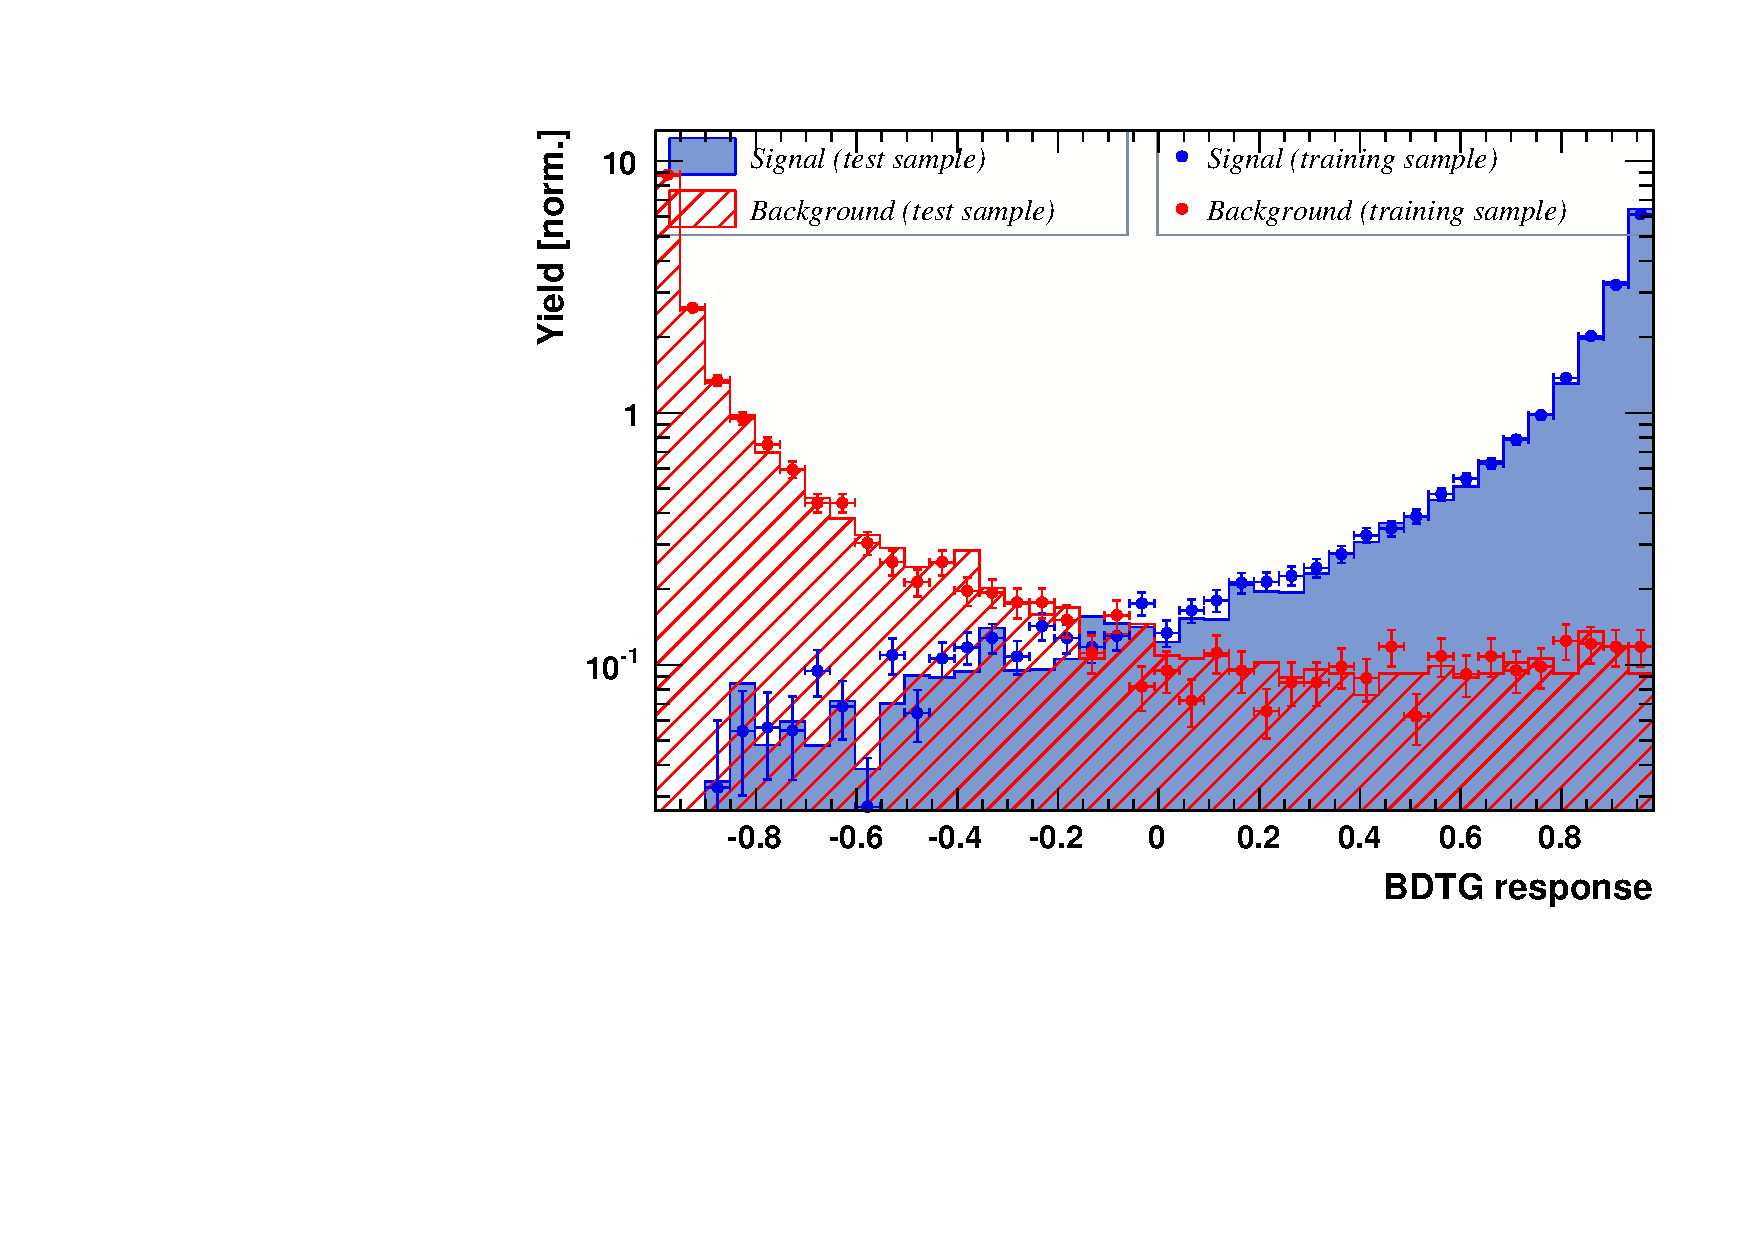
\includegraphics[height=!,width=0.4\textwidth]{figs/TMVA/BDTG_Data_run2_t0_odd/overtrain_BDTG.pdf}
\caption{Response of the classifier trained on the even and tested on the odd sample (left) and trained on the odd and tested on the even sample (right) for category [Run-II,\textsf{L0-TOS}].}

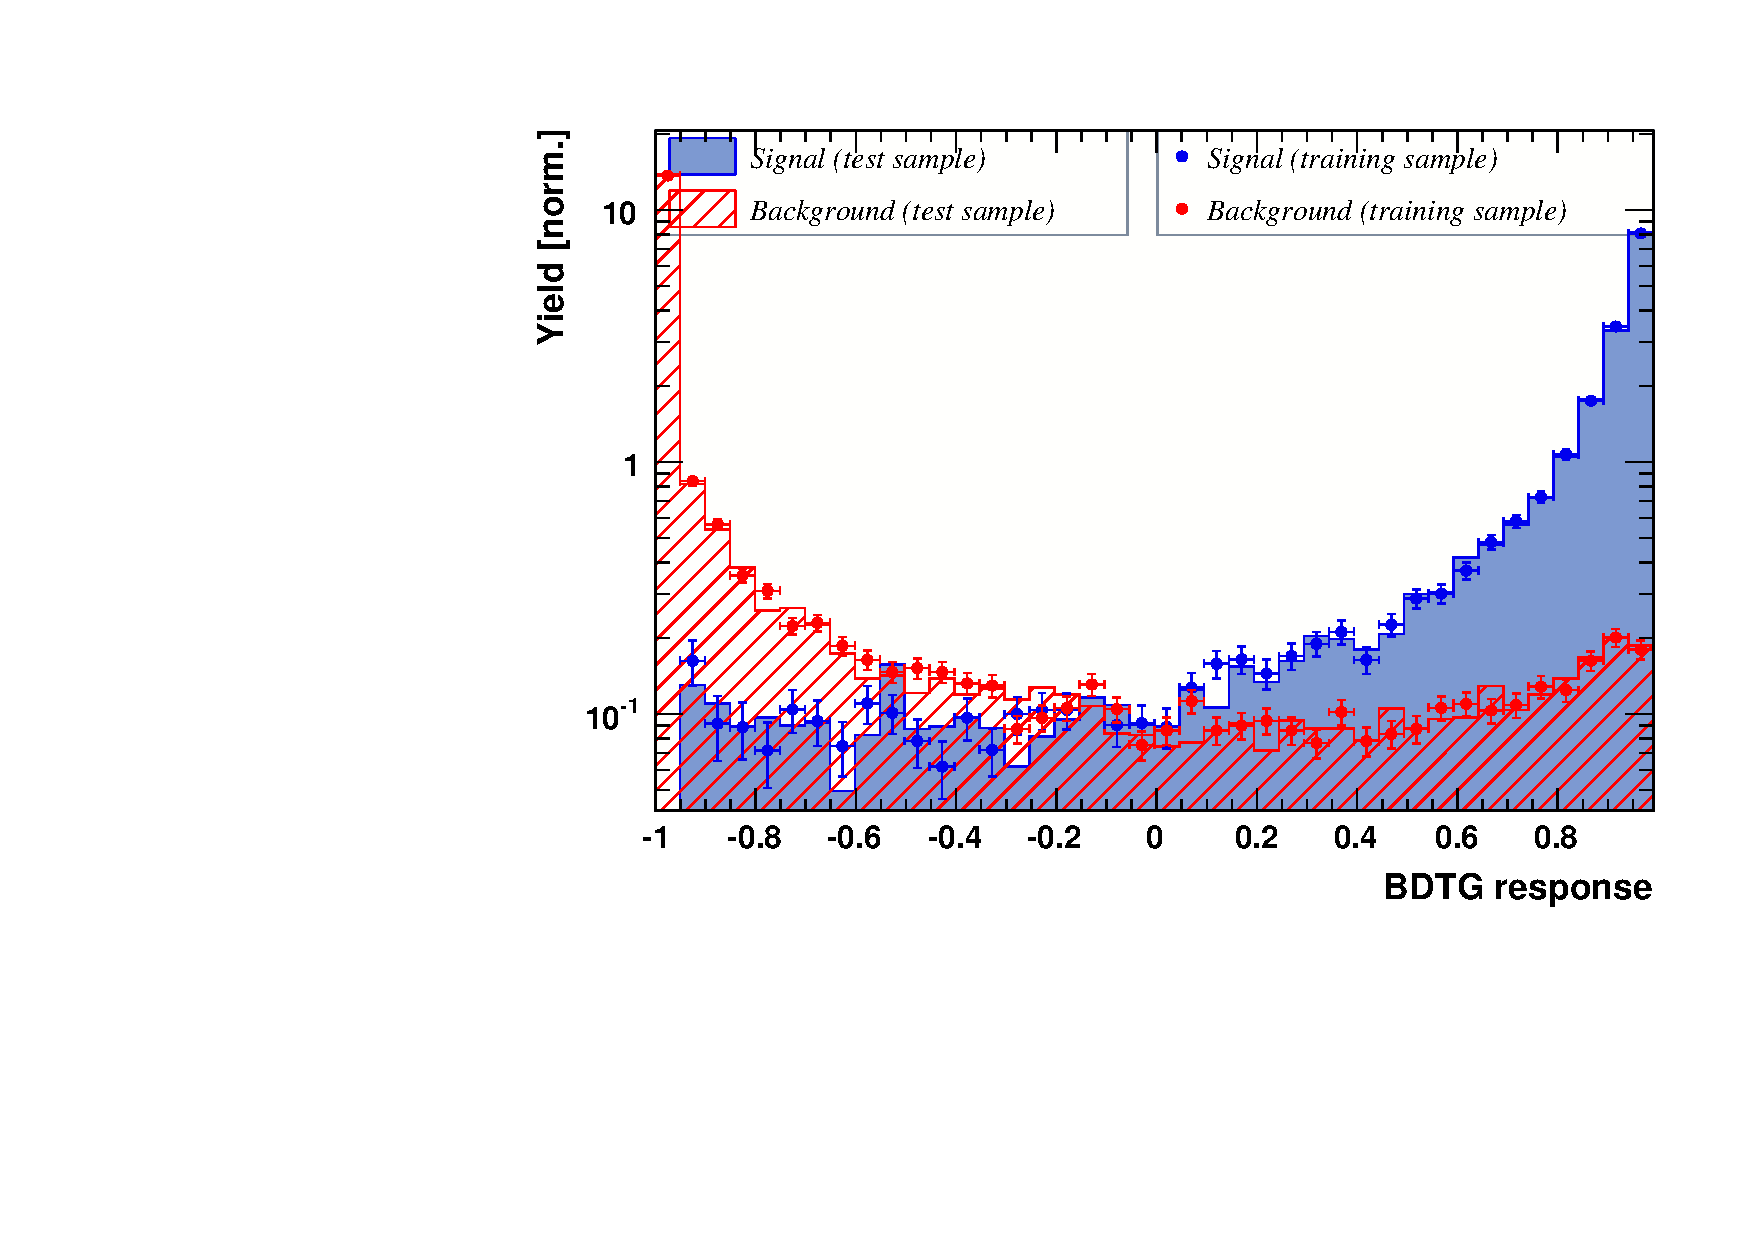
\includegraphics[height=!,width=0.4\textwidth]{figs/TMVA/BDTG_Data_run2_t1_even/overtrain_BDTG.pdf}
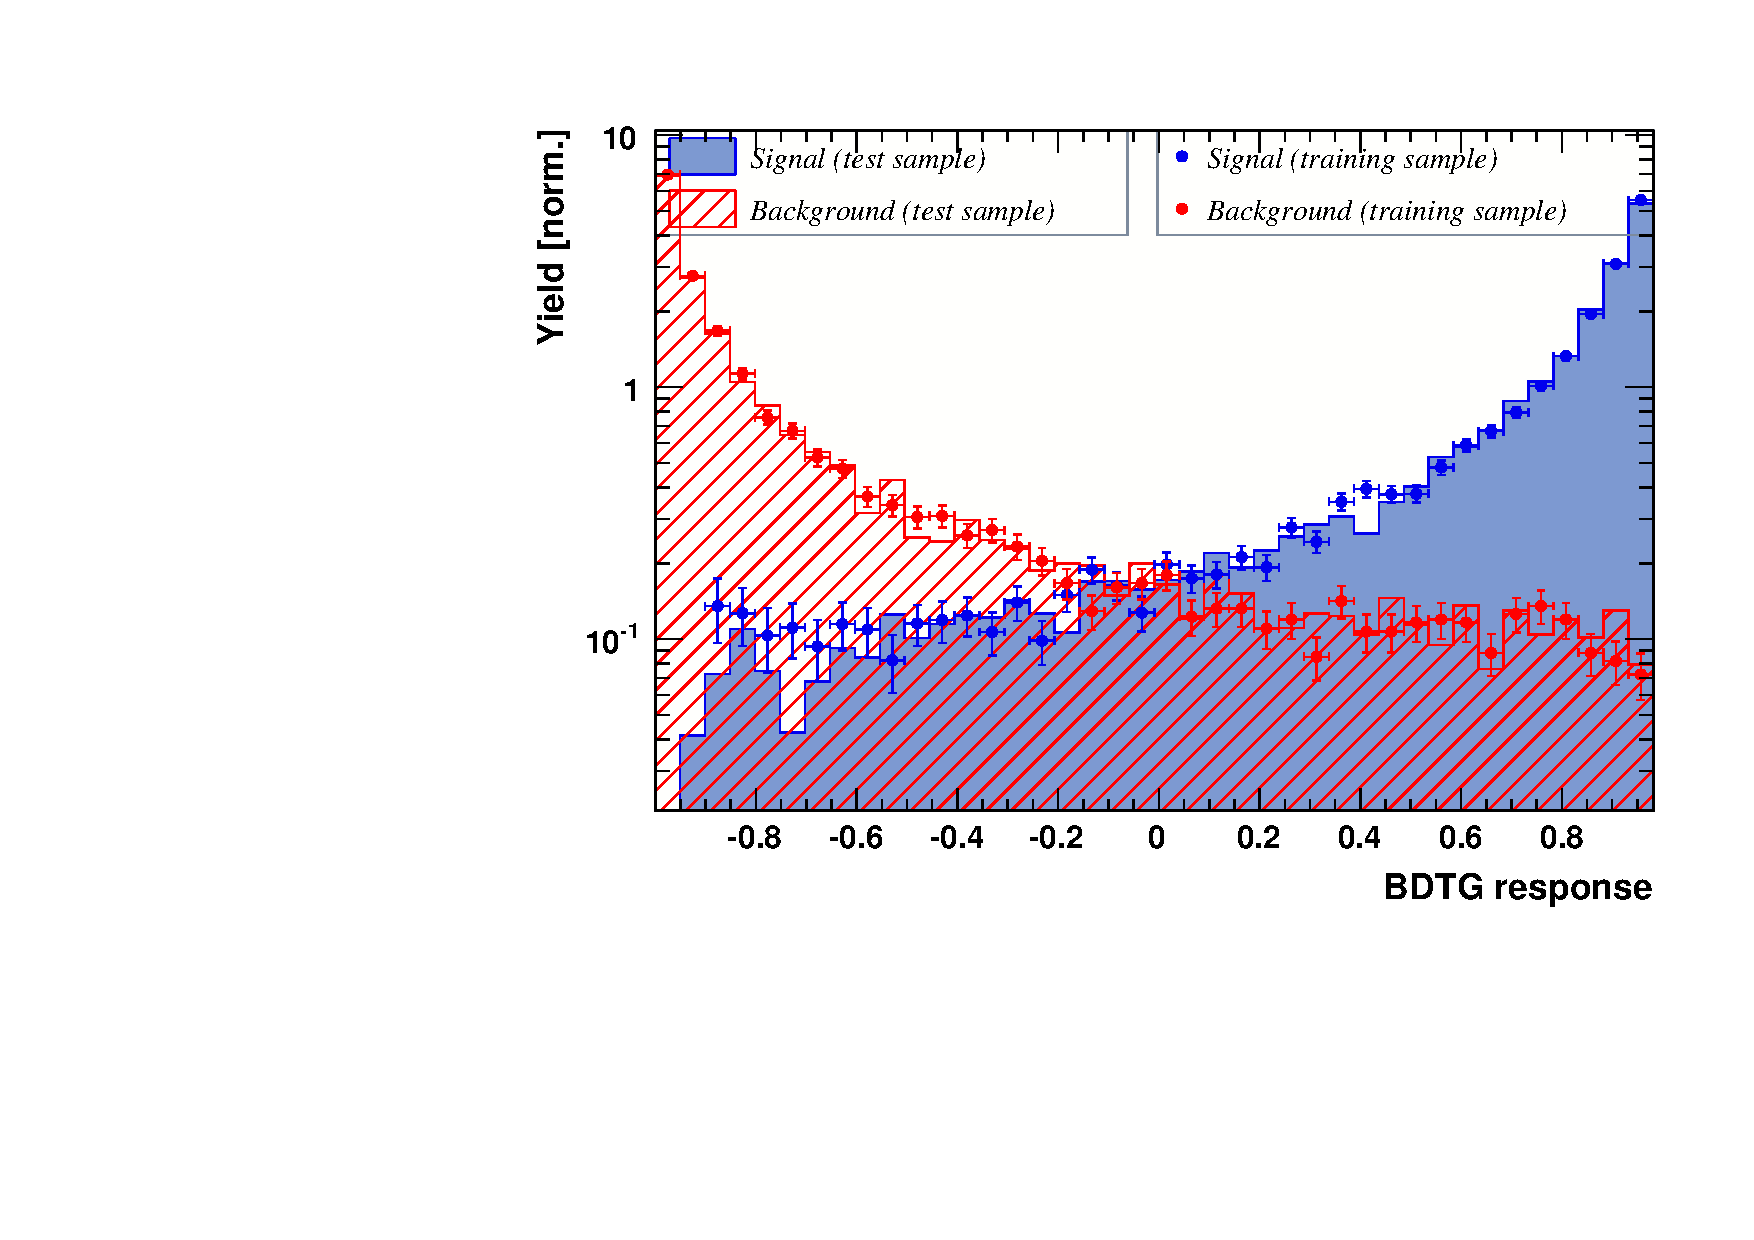
\includegraphics[height=!,width=0.4\textwidth]{figs/TMVA/BDTG_Data_run2_t1_odd/overtrain_BDTG.pdf}
\caption{Response of the classifier trained on the even and tested on the odd sample (left) and trained on the odd and tested on the even sample (right) for category [Run-II,\textsf{L0-TIS}].}
\end{figure}

\begin{figure}[h]
\centering
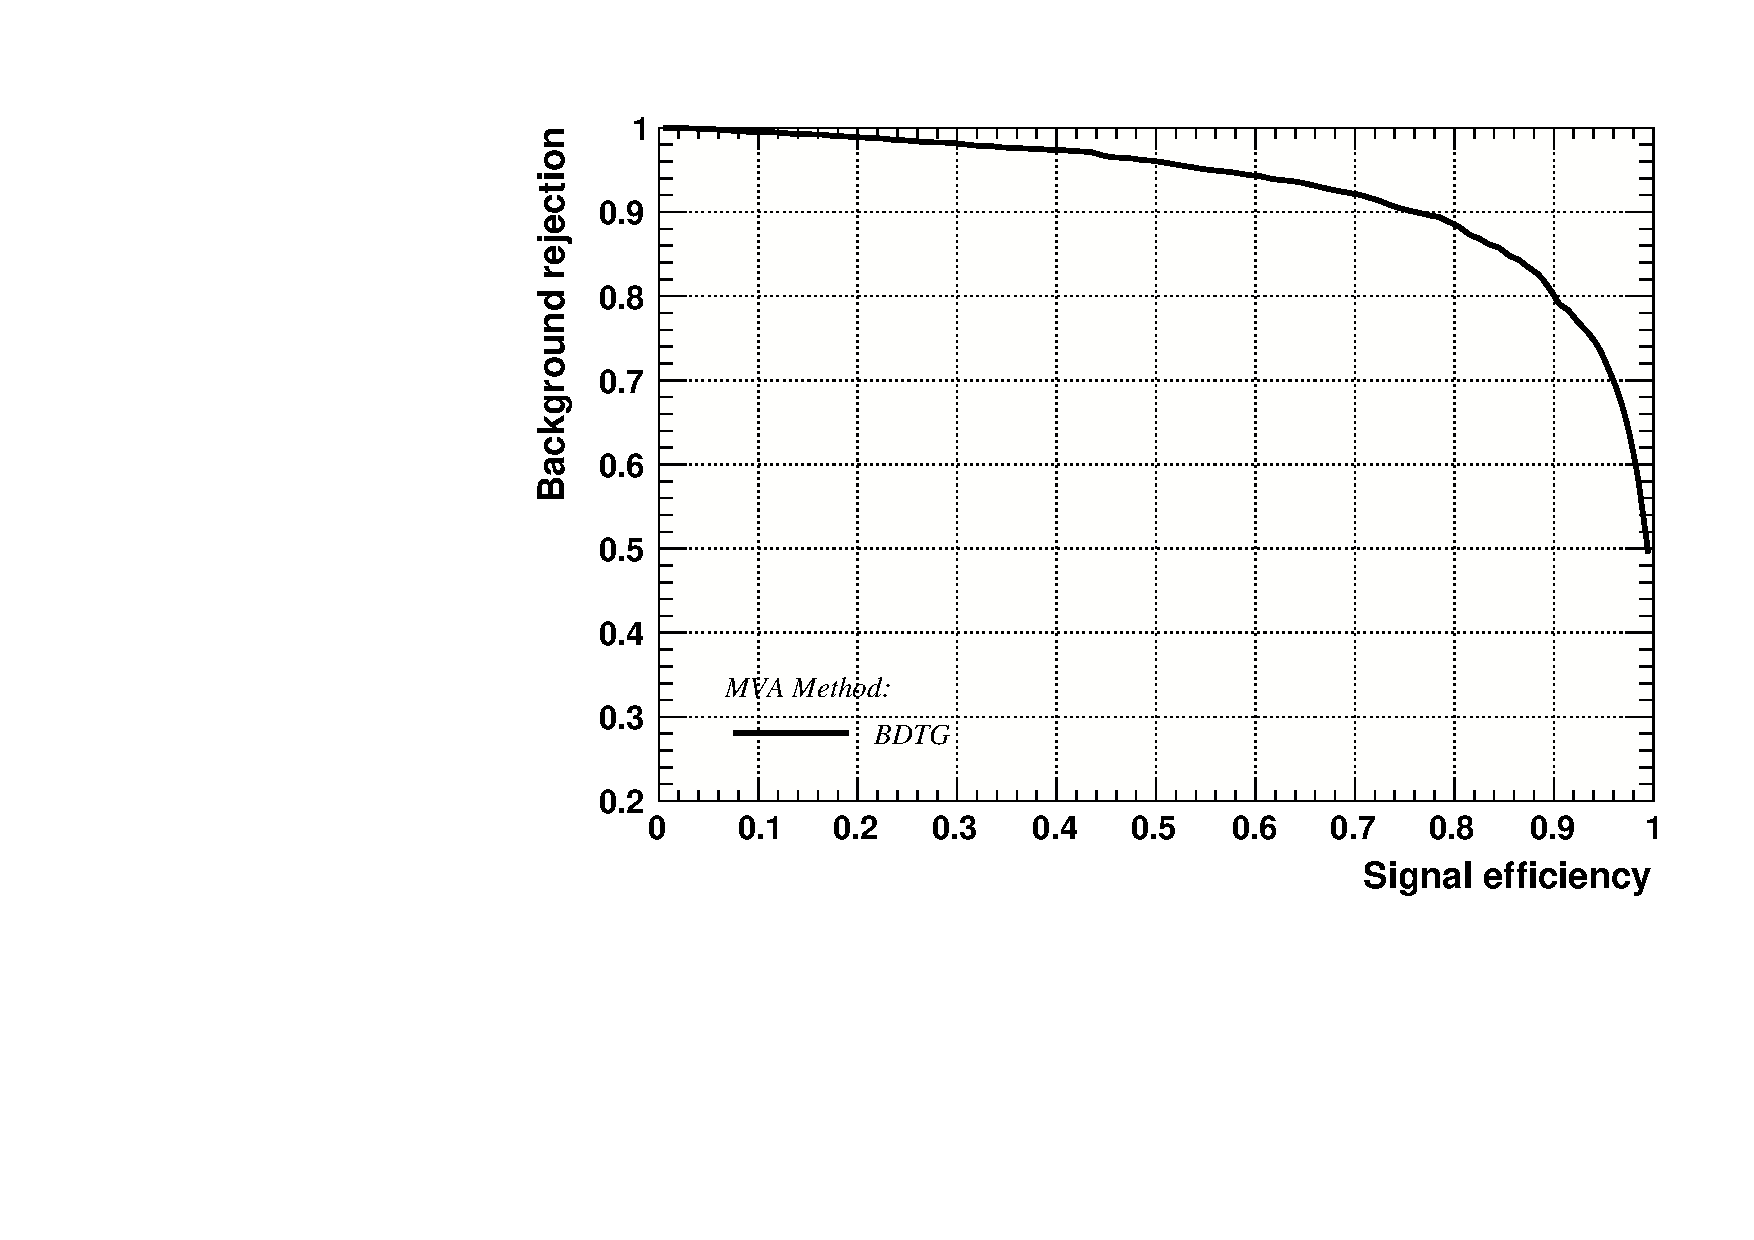
\includegraphics[height=!,width=0.4\textwidth]{figs/TMVA/BDTG_Data_run1_t0_even/rejBvsS.pdf}
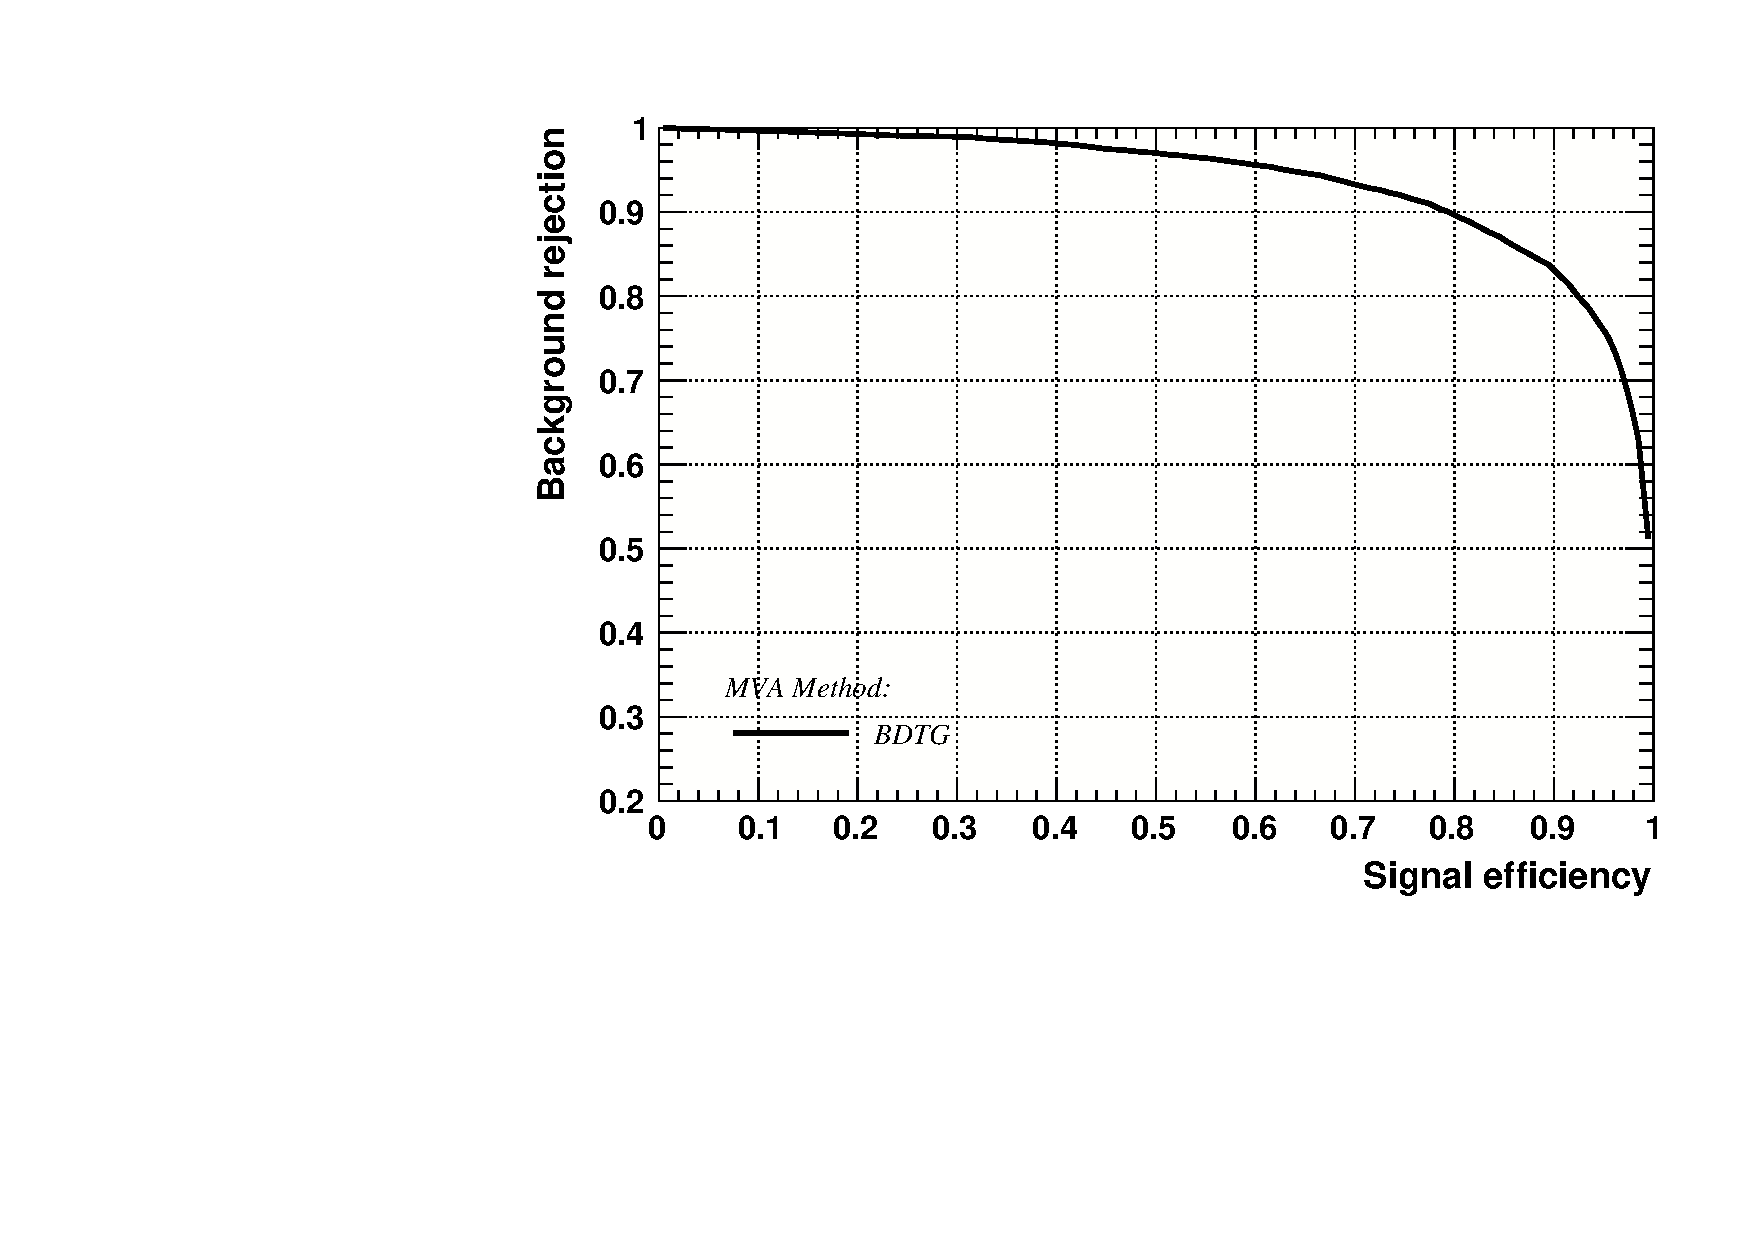
\includegraphics[height=!,width=0.4\textwidth]{figs/TMVA/BDTG_Data_run1_t0_odd/rejBvsS.pdf}
\caption{Signal efficiency versus background rejection for the BDT trained on the even (left) and odd (right) sample for category [Run-I,\textsf{L0-TOS}].}

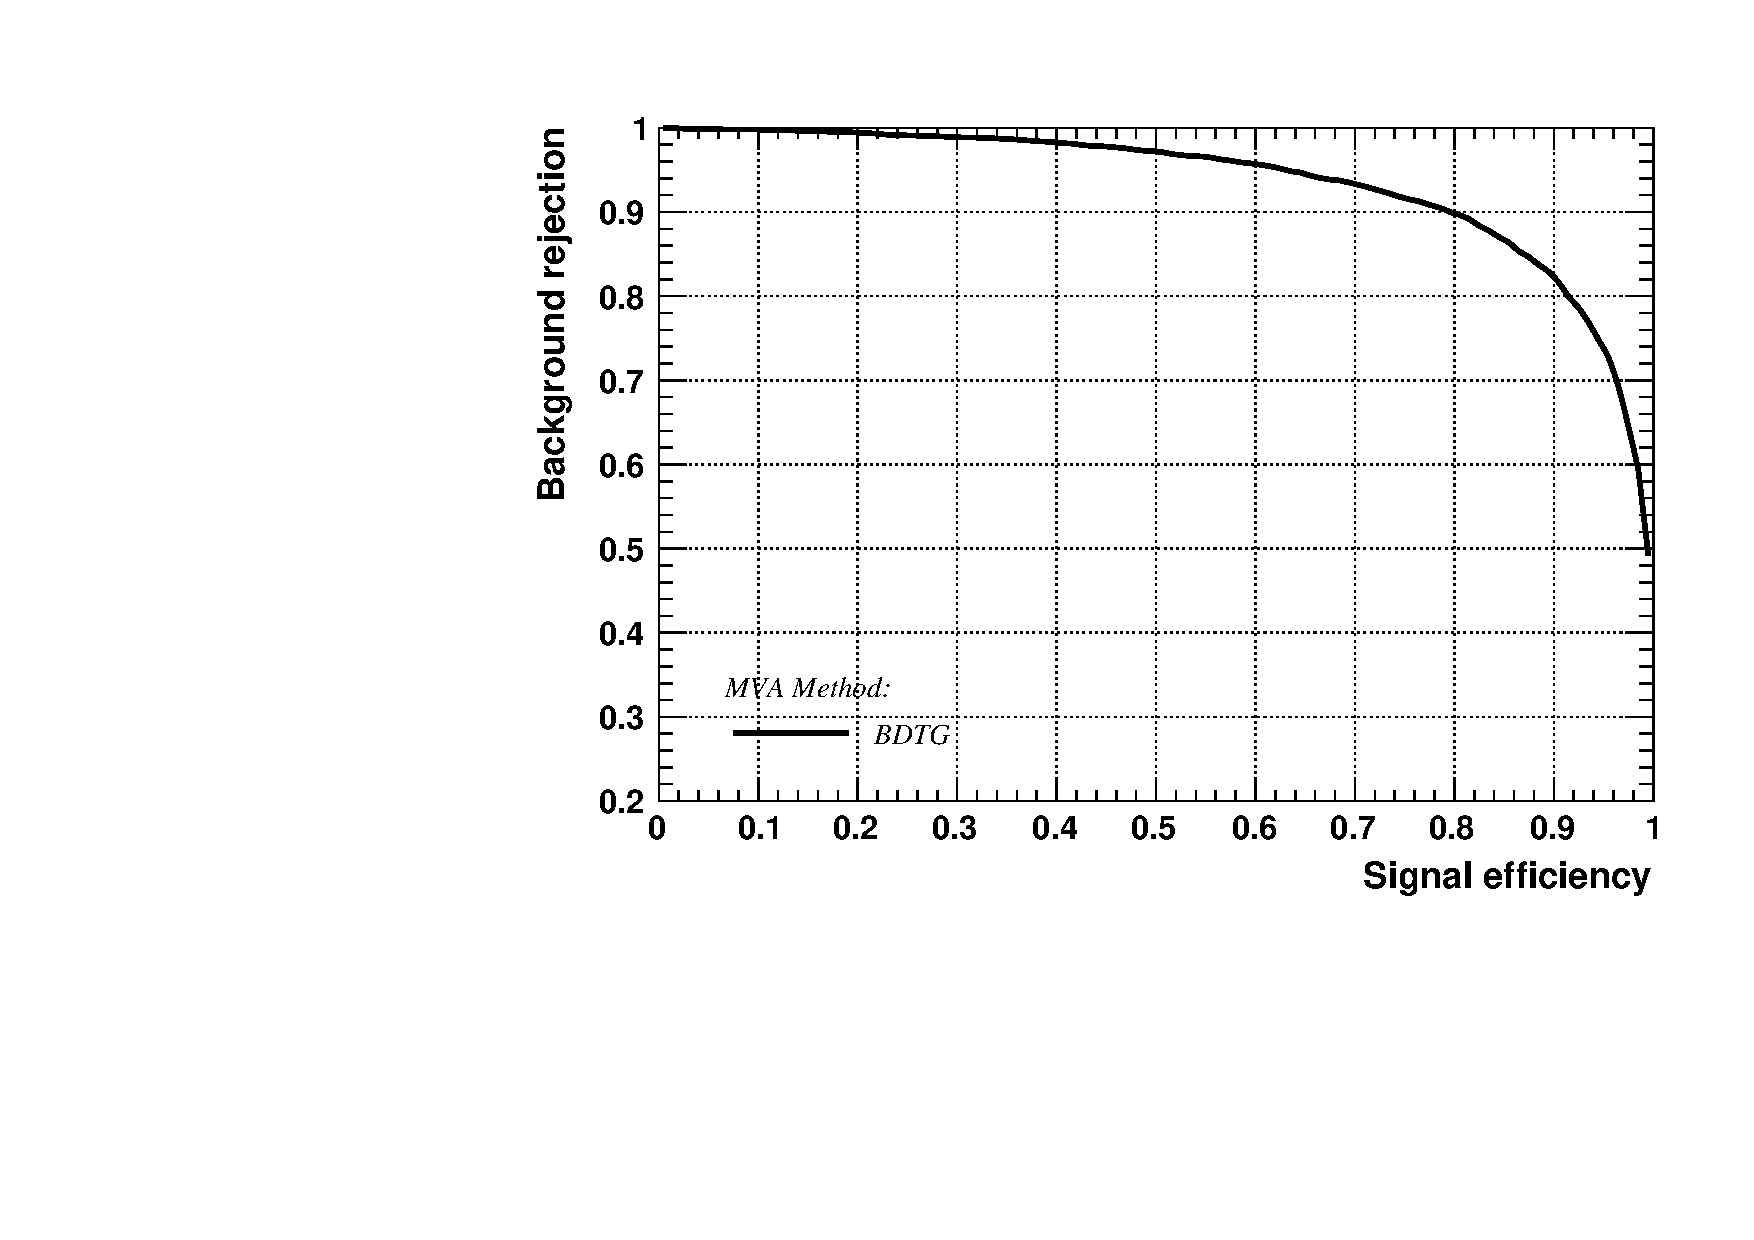
\includegraphics[height=!,width=0.4\textwidth]{figs/TMVA/BDTG_Data_run1_t1_even/rejBvsS.pdf}
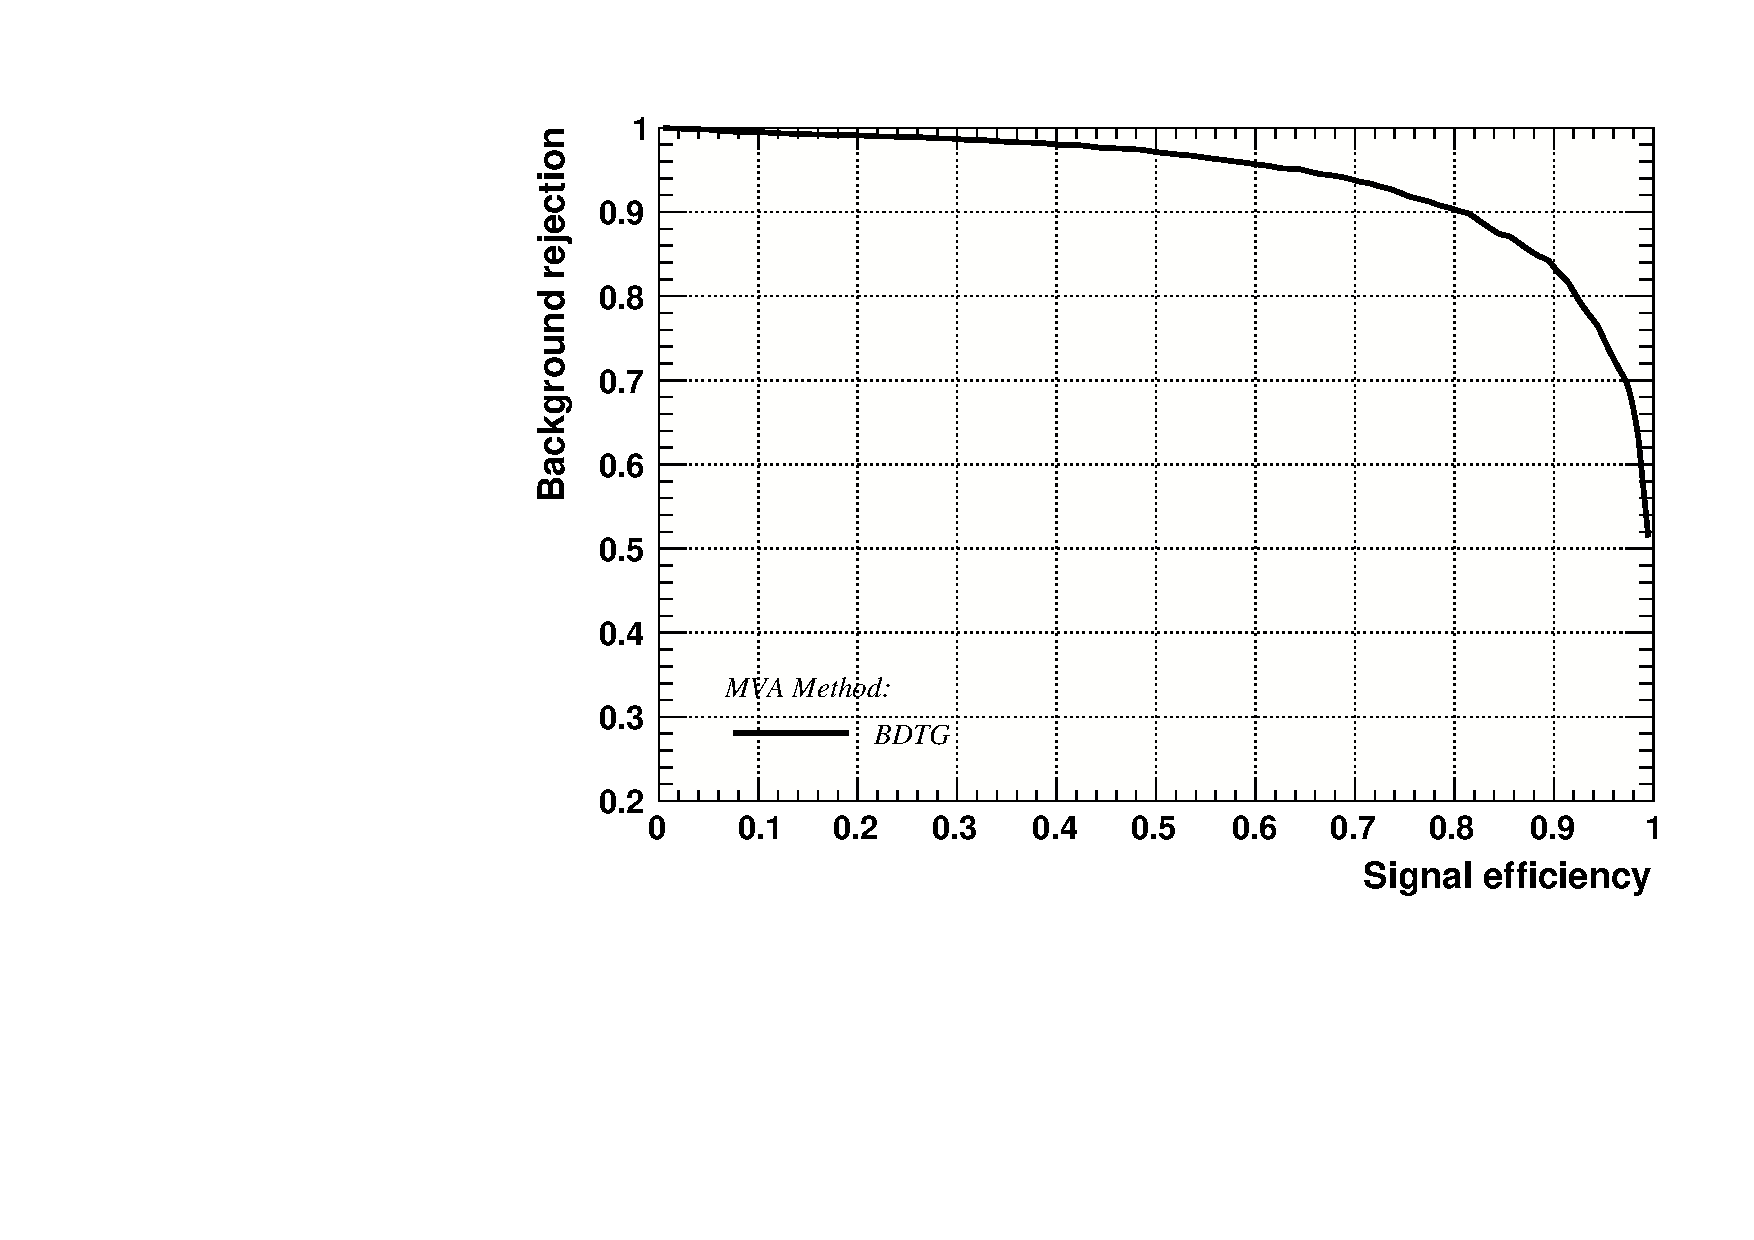
\includegraphics[height=!,width=0.4\textwidth]{figs/TMVA/BDTG_Data_run1_t1_odd/rejBvsS.pdf}
\caption{Signal efficiency versus background rejection for the BDT trained on the even (left) and odd (right) sample for category [Run-I,\textsf{L0-TIS}].}

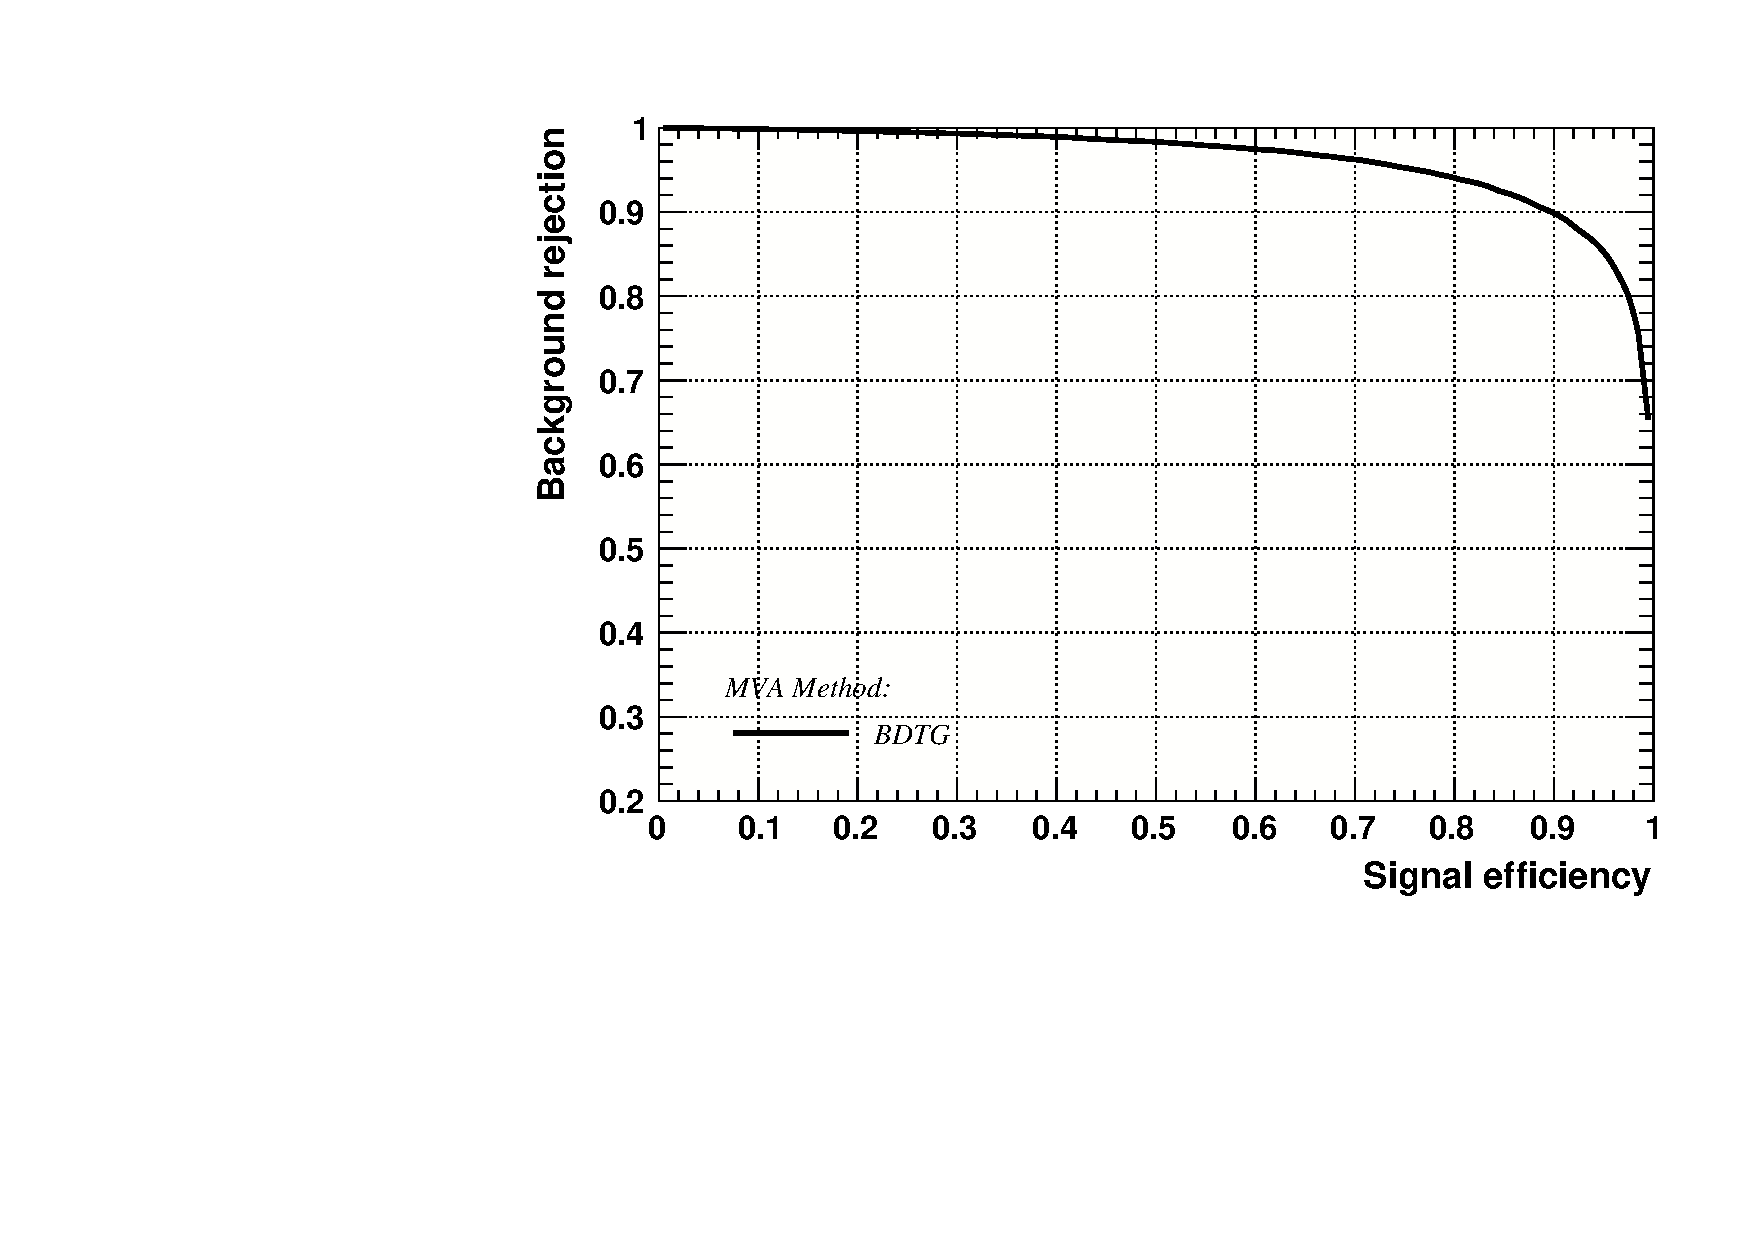
\includegraphics[height=!,width=0.4\textwidth]{figs/TMVA/BDTG_Data_run2_t0_even/rejBvsS.pdf}
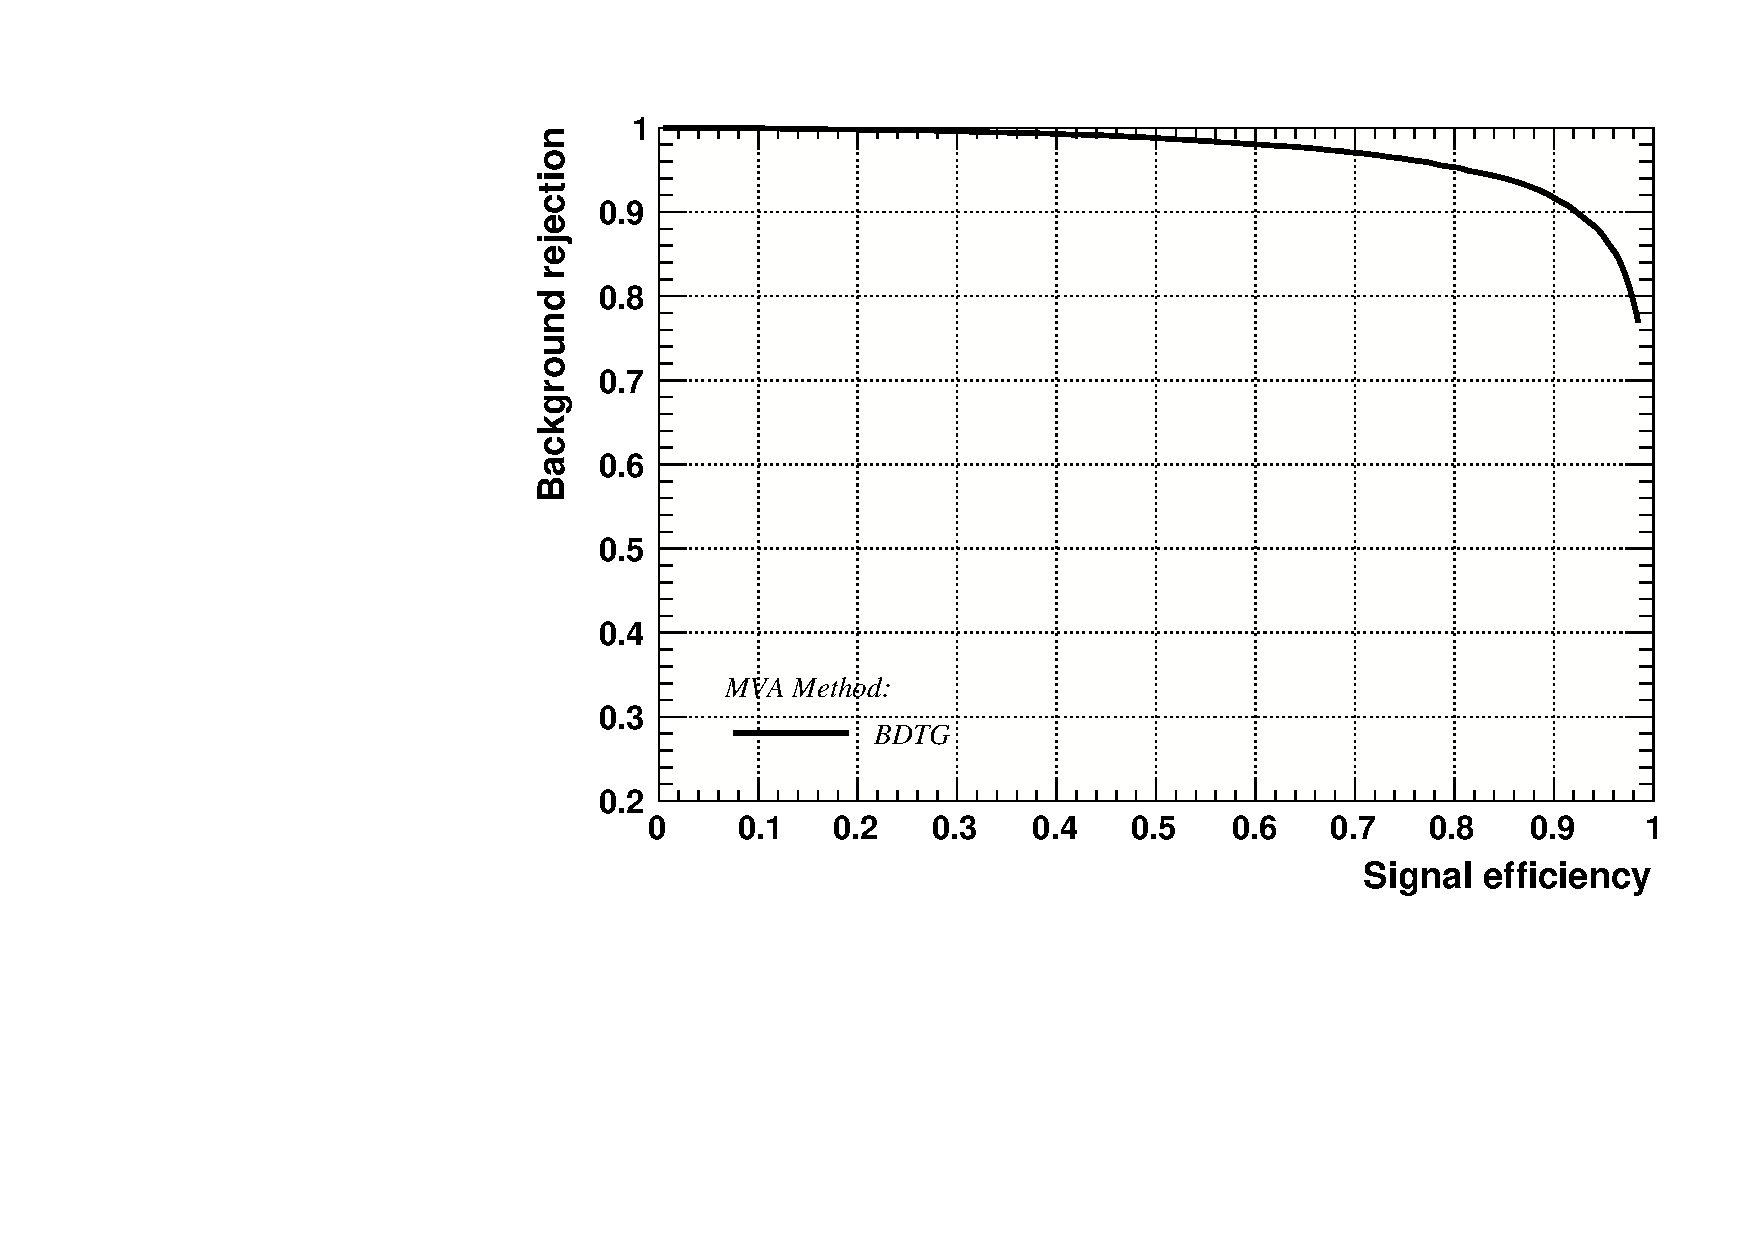
\includegraphics[height=!,width=0.4\textwidth]{figs/TMVA/BDTG_Data_run2_t0_odd/rejBvsS.pdf}
\caption{Signal efficiency versus background rejection for the BDT trained on the even (left) and odd (right) sample for category [Run-II,\textsf{L0-TOS}].}

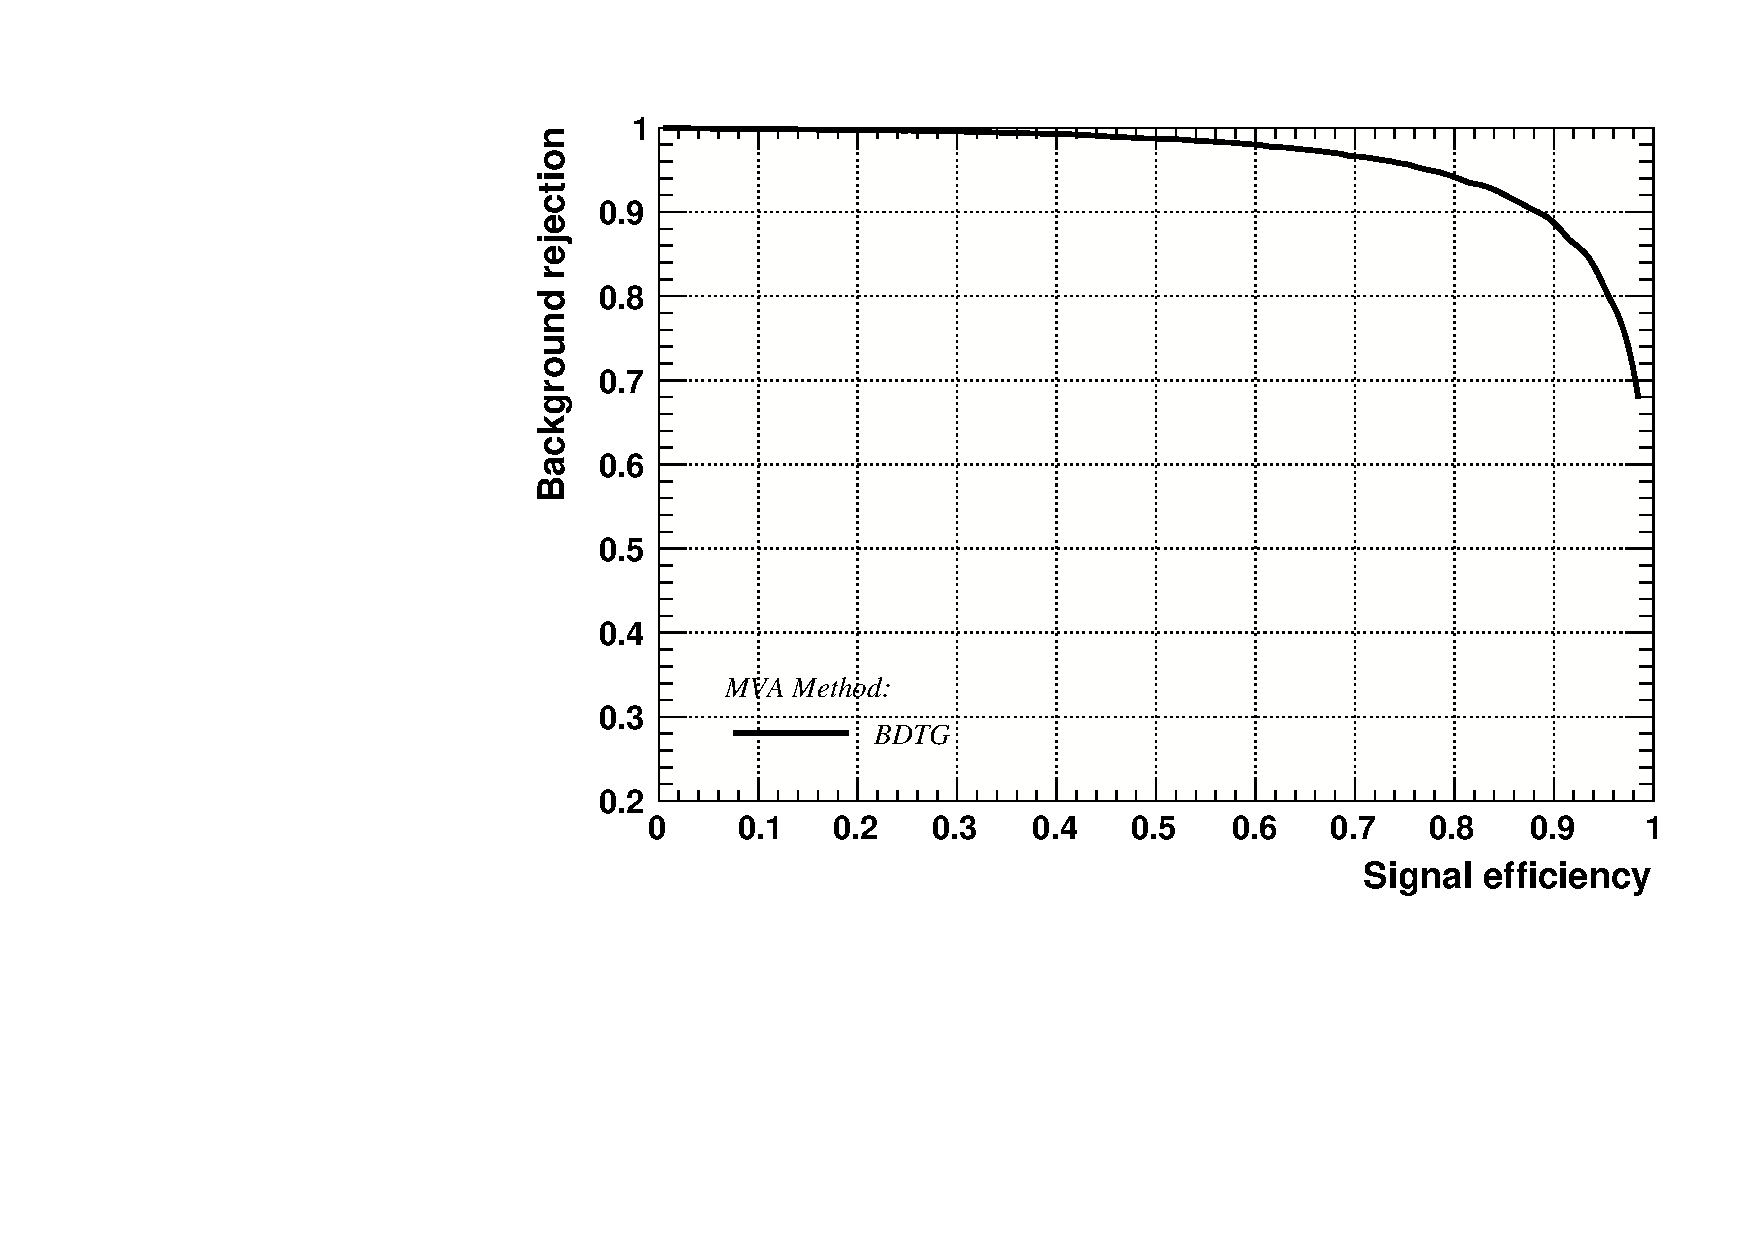
\includegraphics[height=!,width=0.4\textwidth]{figs/TMVA/BDTG_Data_run2_t1_even/rejBvsS.pdf}
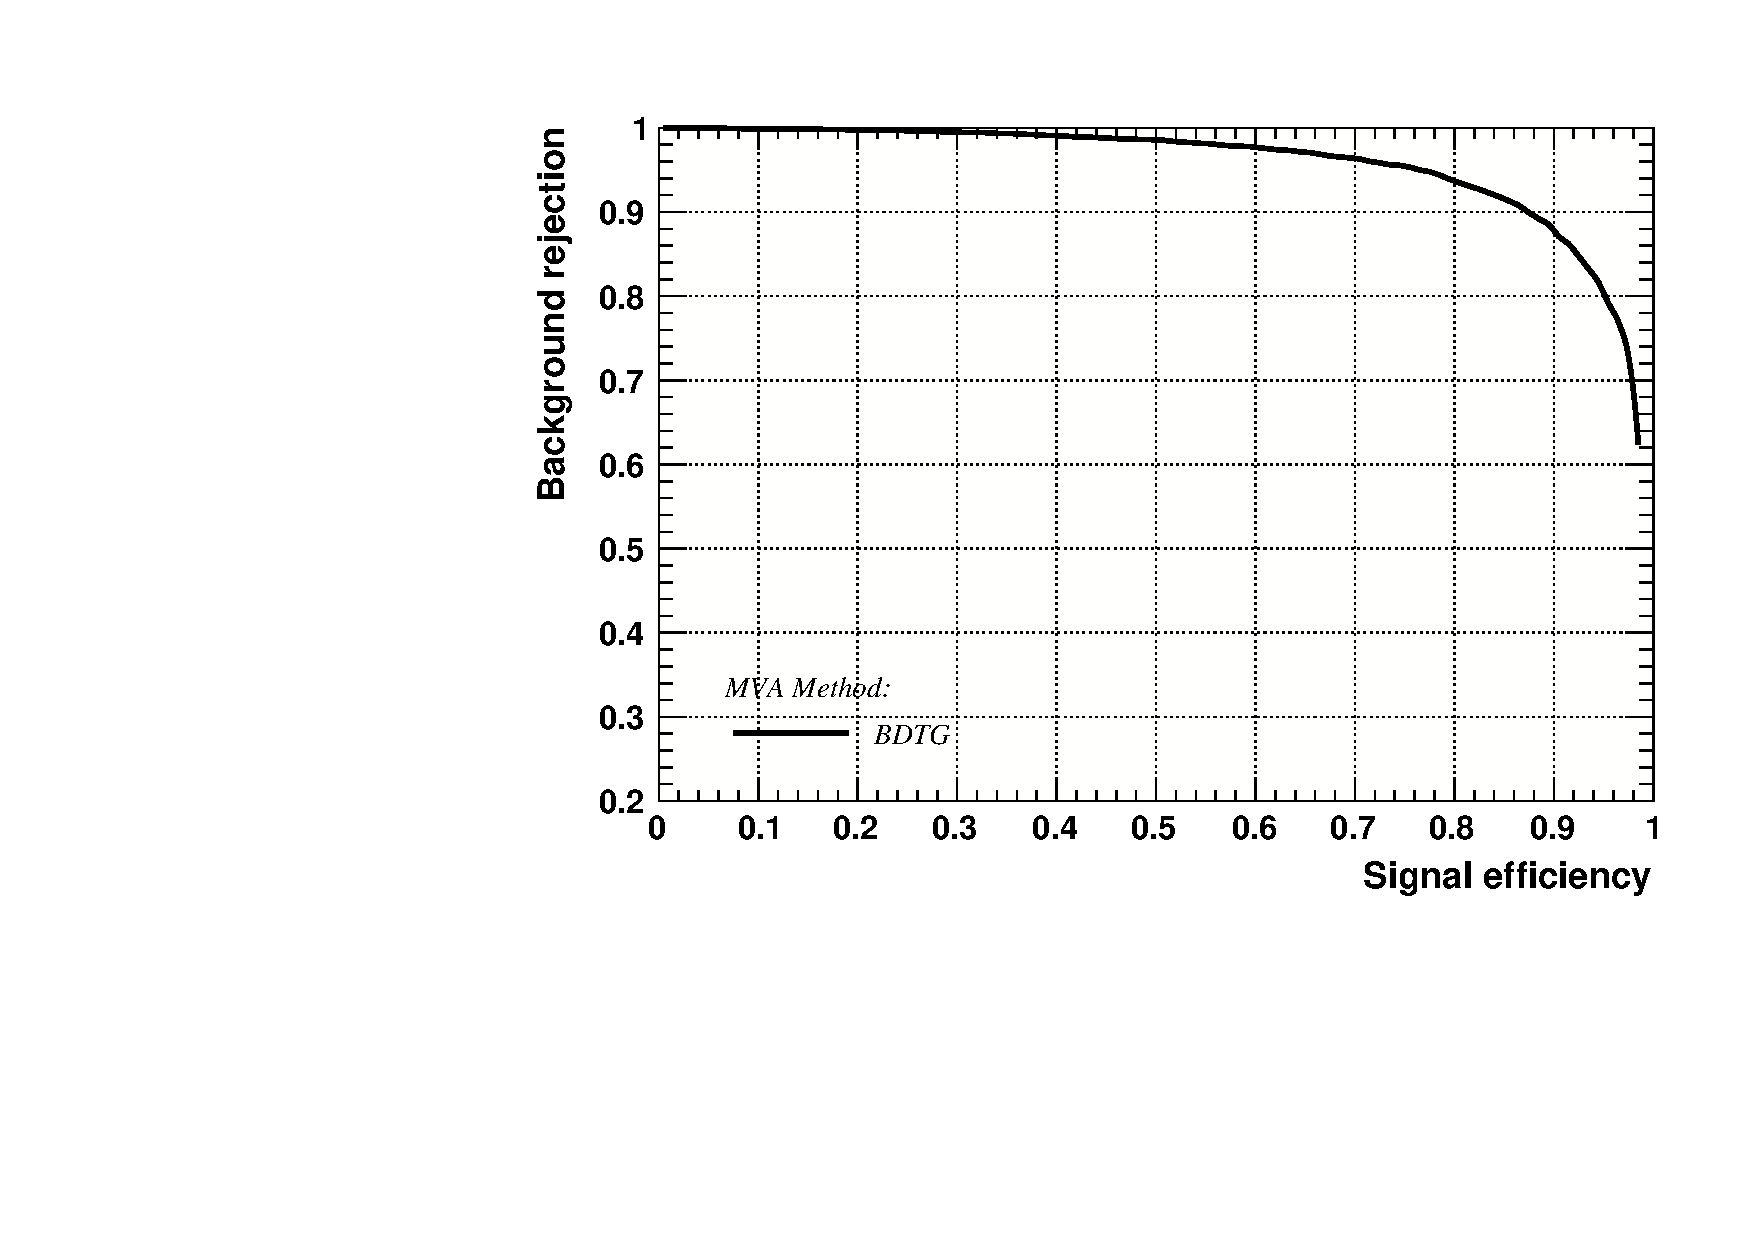
\includegraphics[height=!,width=0.4\textwidth]{figs/TMVA/BDTG_Data_run2_t1_odd/rejBvsS.pdf}
\caption{Signal efficiency versus background rejection for the BDT trained on the even (left) and odd (right) sample for category[Run-II,\textsf{L0-TIS}].}
\end{figure}


\clearpage
\section{Detailed mass fits}
\label{sec:DetailedMassfits}

\setcounter{figure}{0}
\setcounter{table}{0}

\renewcommand{\thefigure}{B.\arabic{figure}}

In this section, all fits to the mass distribution of $\Bs\to\Ds\pion\pion\pion$ and $\Bs\to\Ds\kaon\pion\pion$ candidates are shown. 
The fits are performed simultaneously 
in run period (Run-I, Run-II), 
$\Ds$ final state  ($\Ds\to\kaon\kaon\pion$ non-resonant, $\Ds\to\phi\pi$, $\Ds\to\Kstar\kaon$, or $\Ds\to\pion\pion\pion$) 
and \textsf{L0} trigger category. 

\begin{figure}[h]
\centering
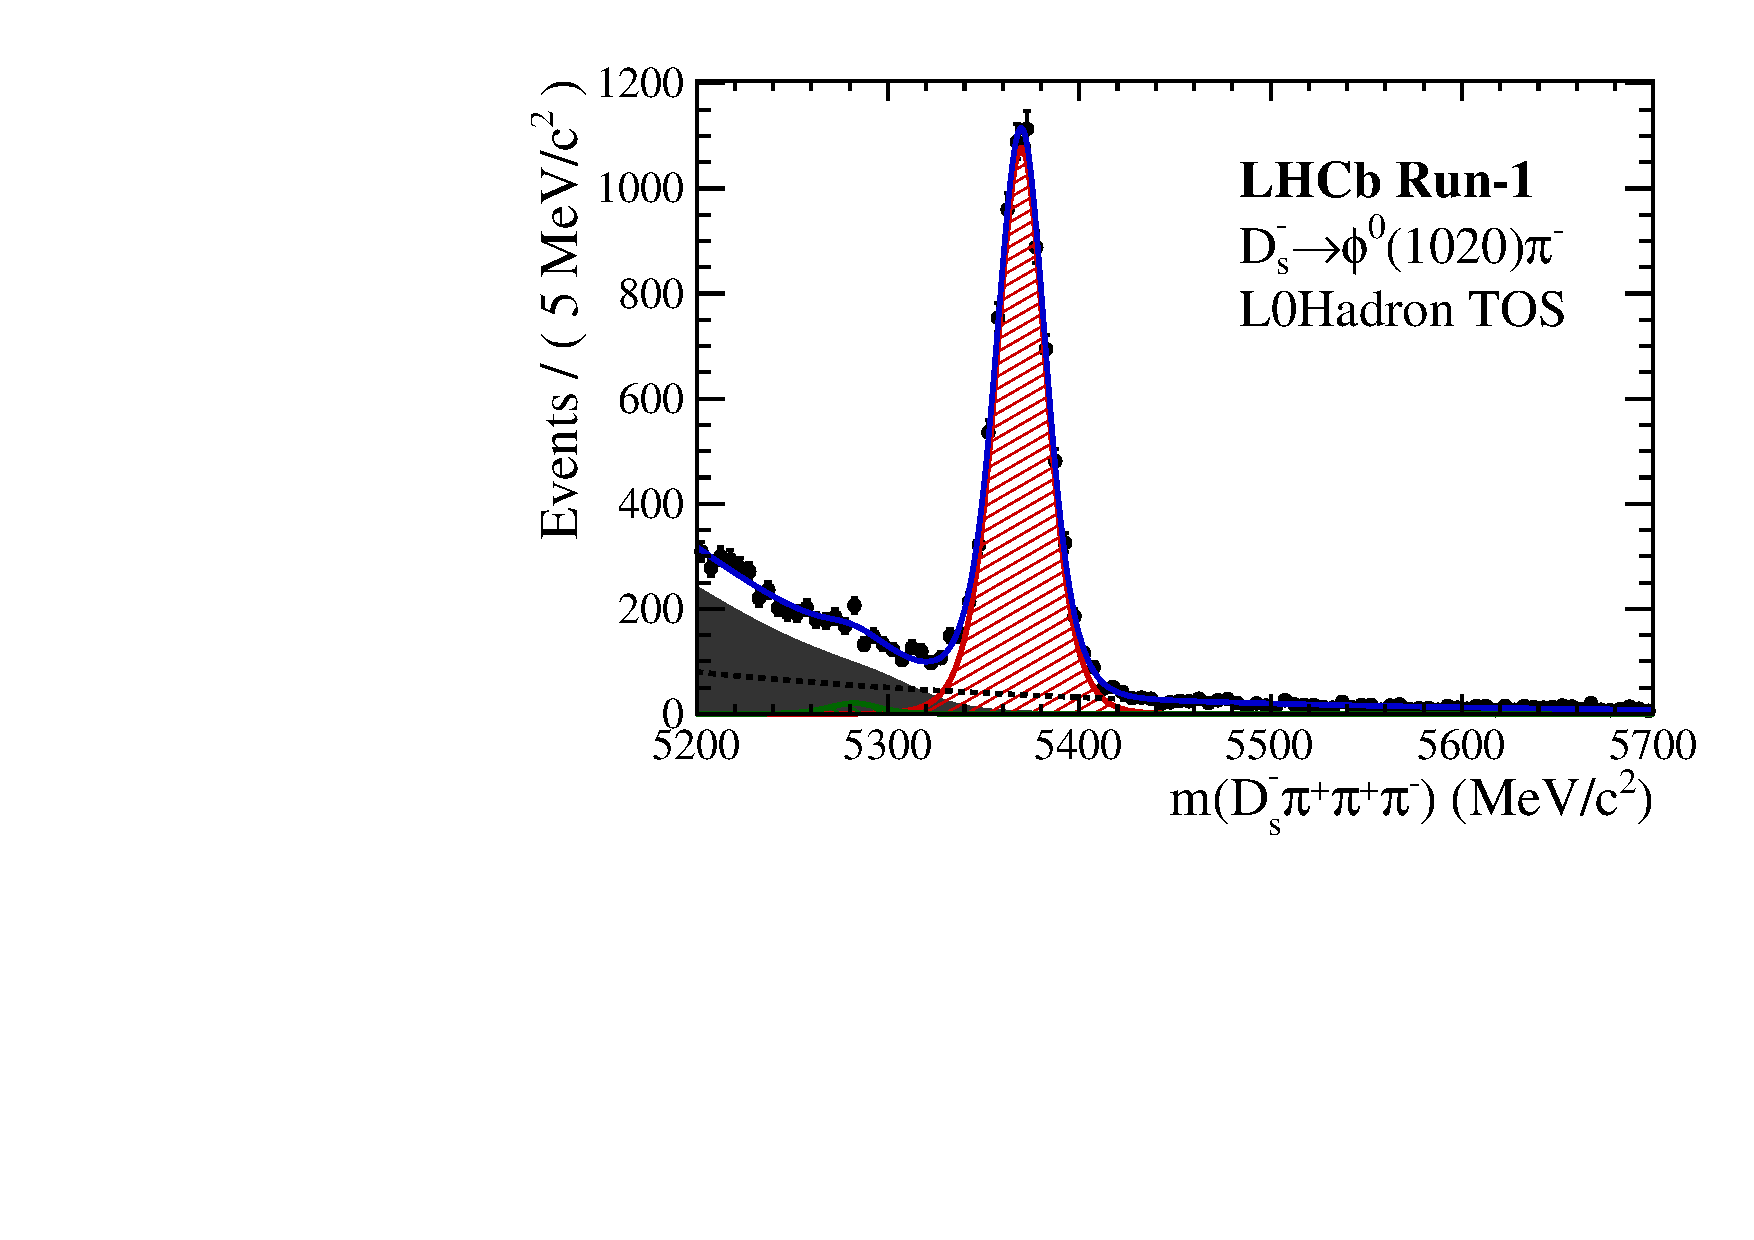
\includegraphics[height=!,width=0.4\textwidth]{figs/MassFit/norm_Run1_phipi_t0.pdf}
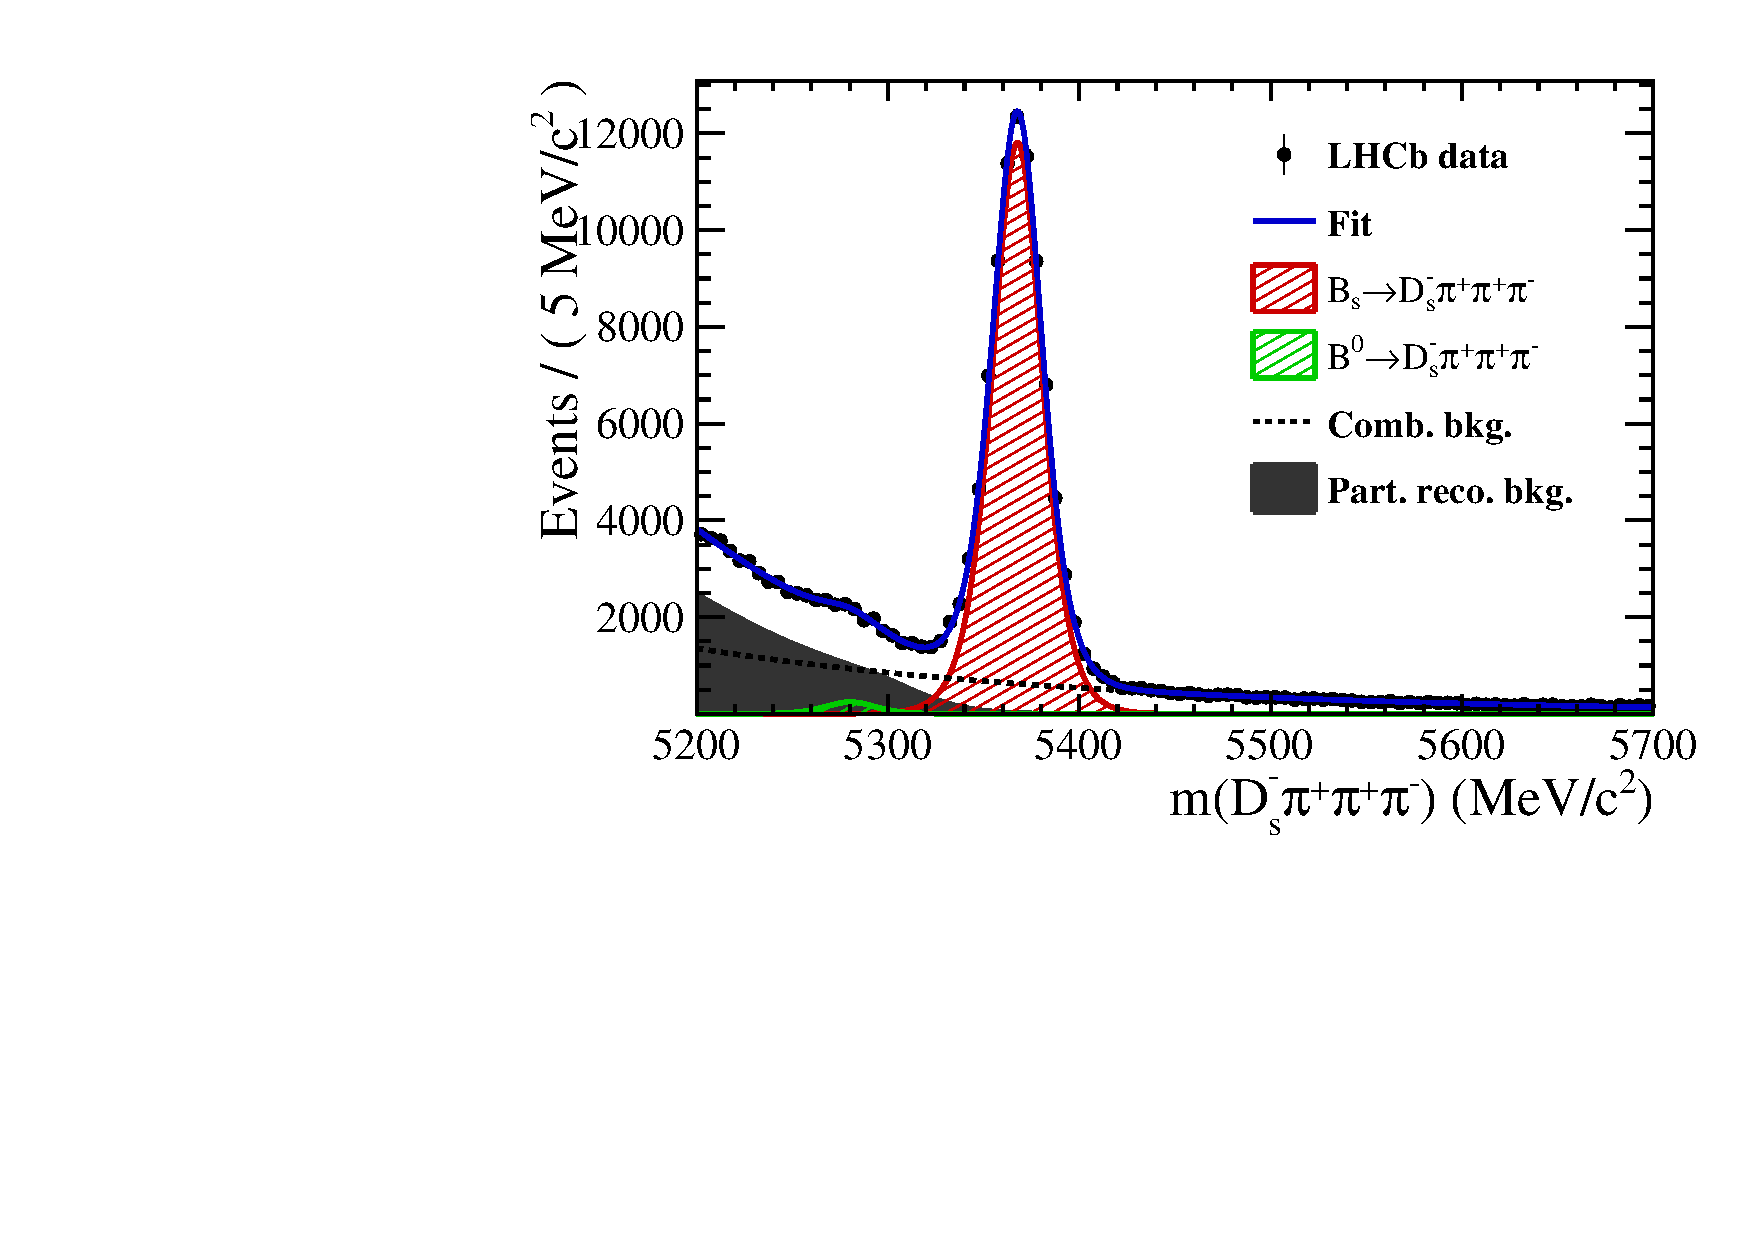
\includegraphics[height=!,width=0.4\textwidth]{figs/MassFit/norm_Run1_phipi_t1.pdf}

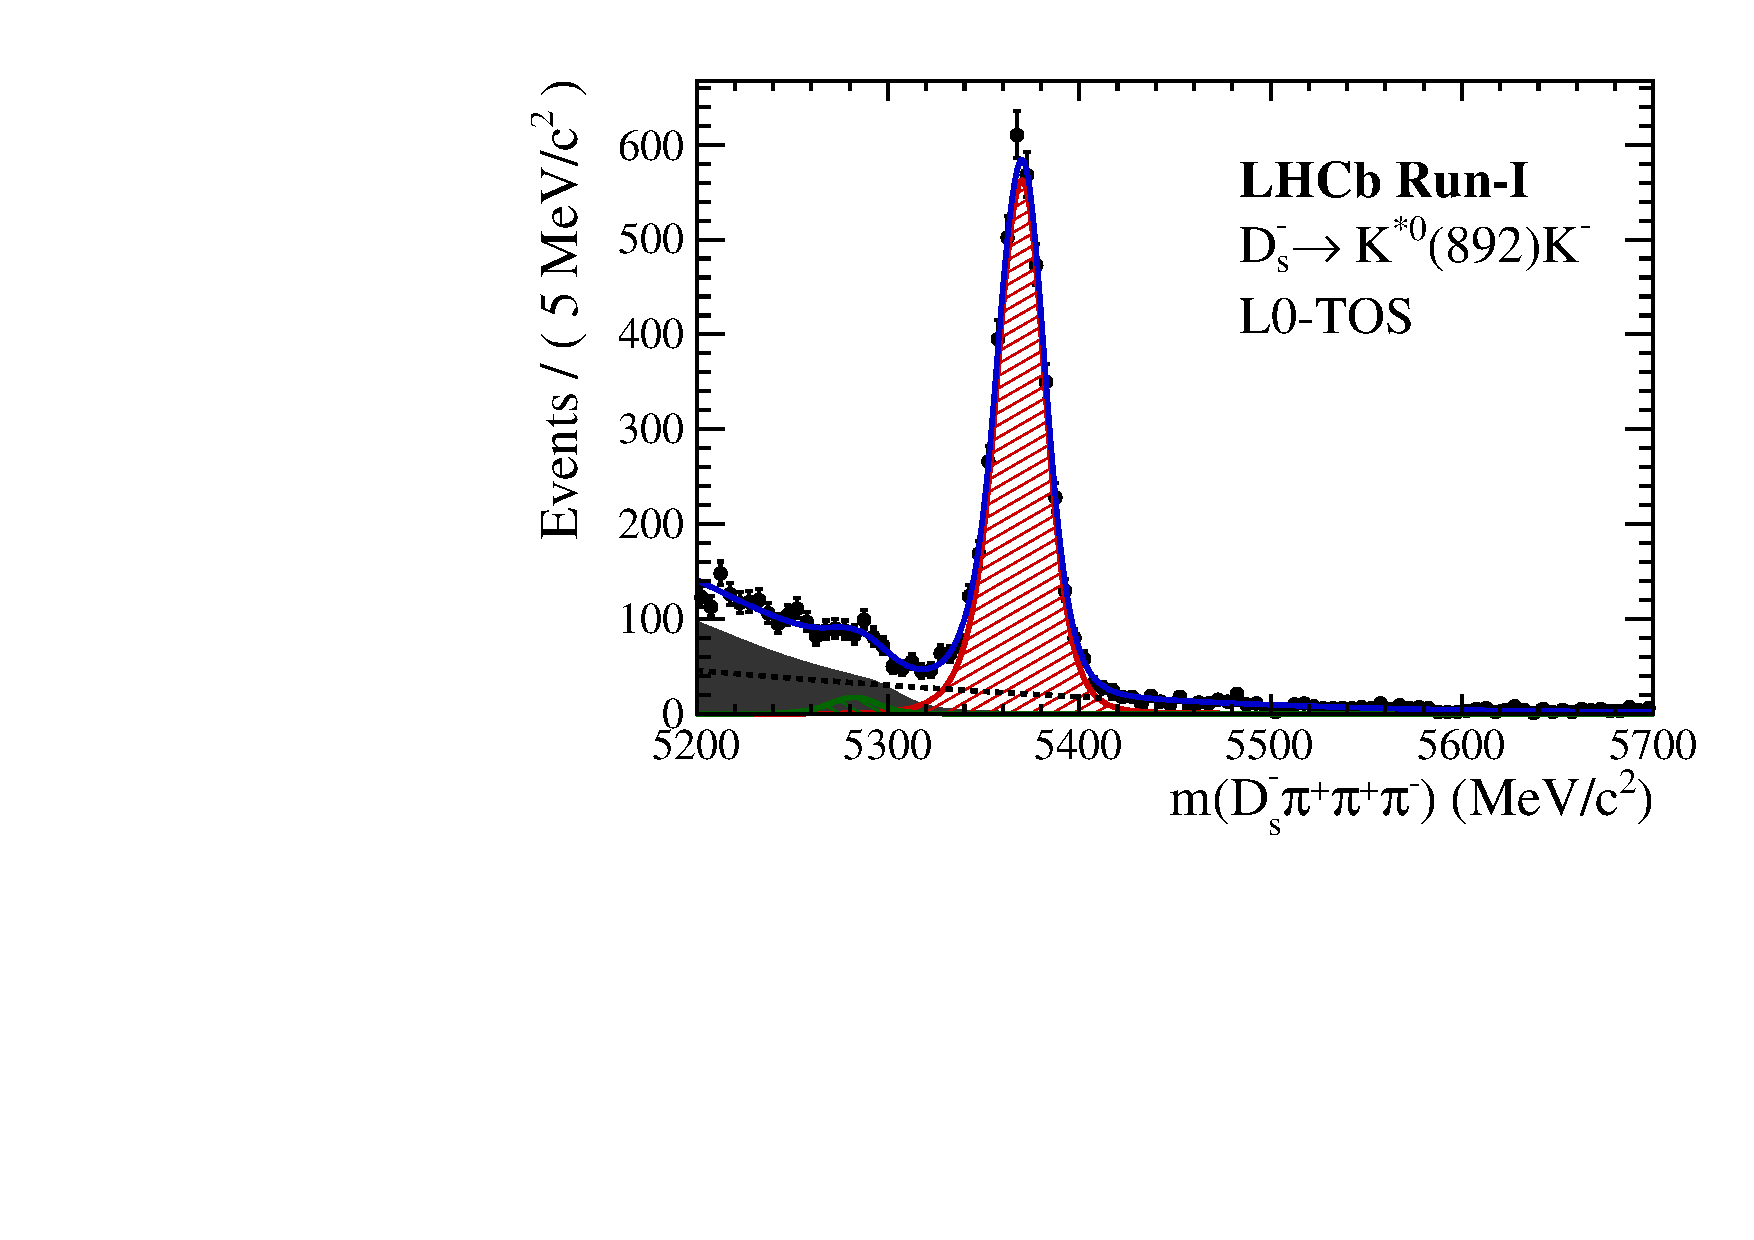
\includegraphics[height=!,width=0.4\textwidth]{figs/MassFit/norm_Run1_KsK_t0.pdf}
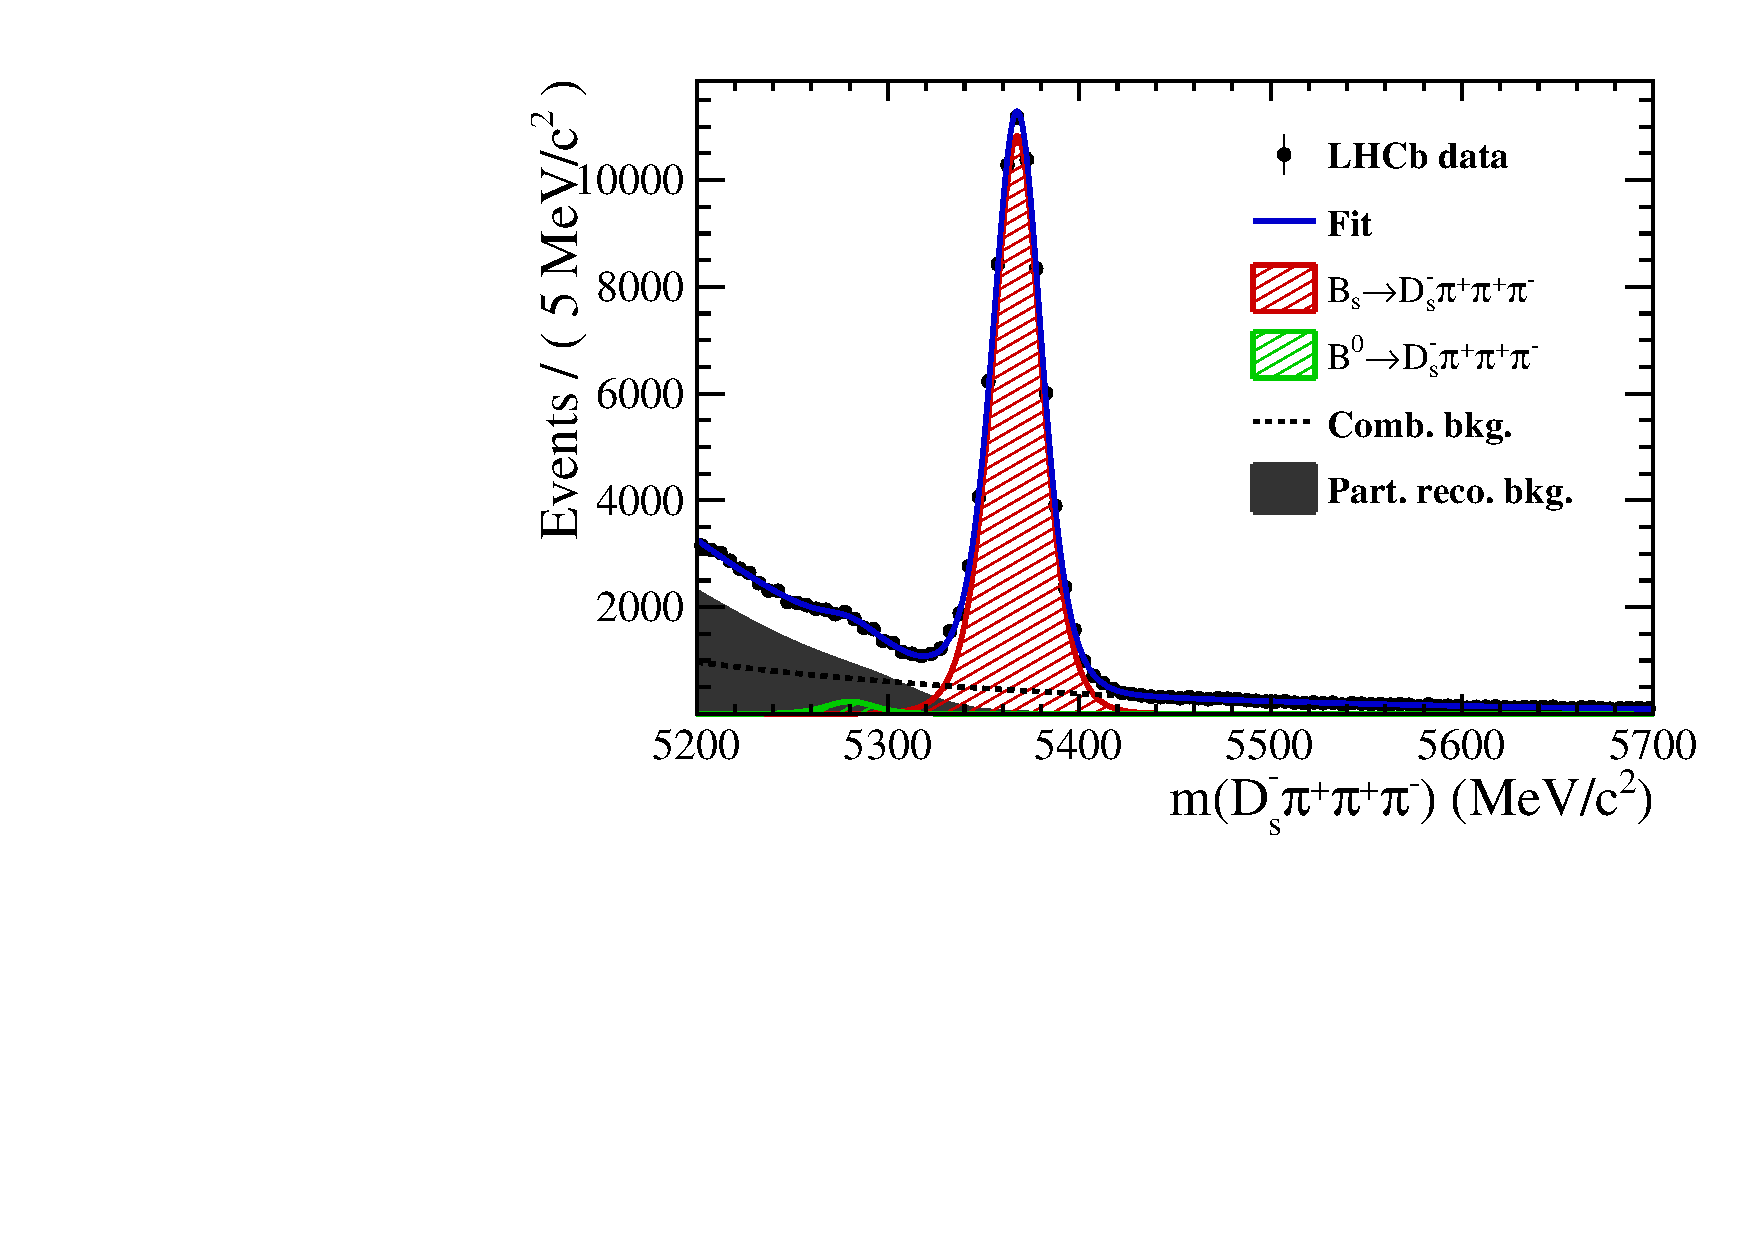
\includegraphics[height=!,width=0.4\textwidth]{figs/MassFit/norm_Run1_KsK_t1.pdf}

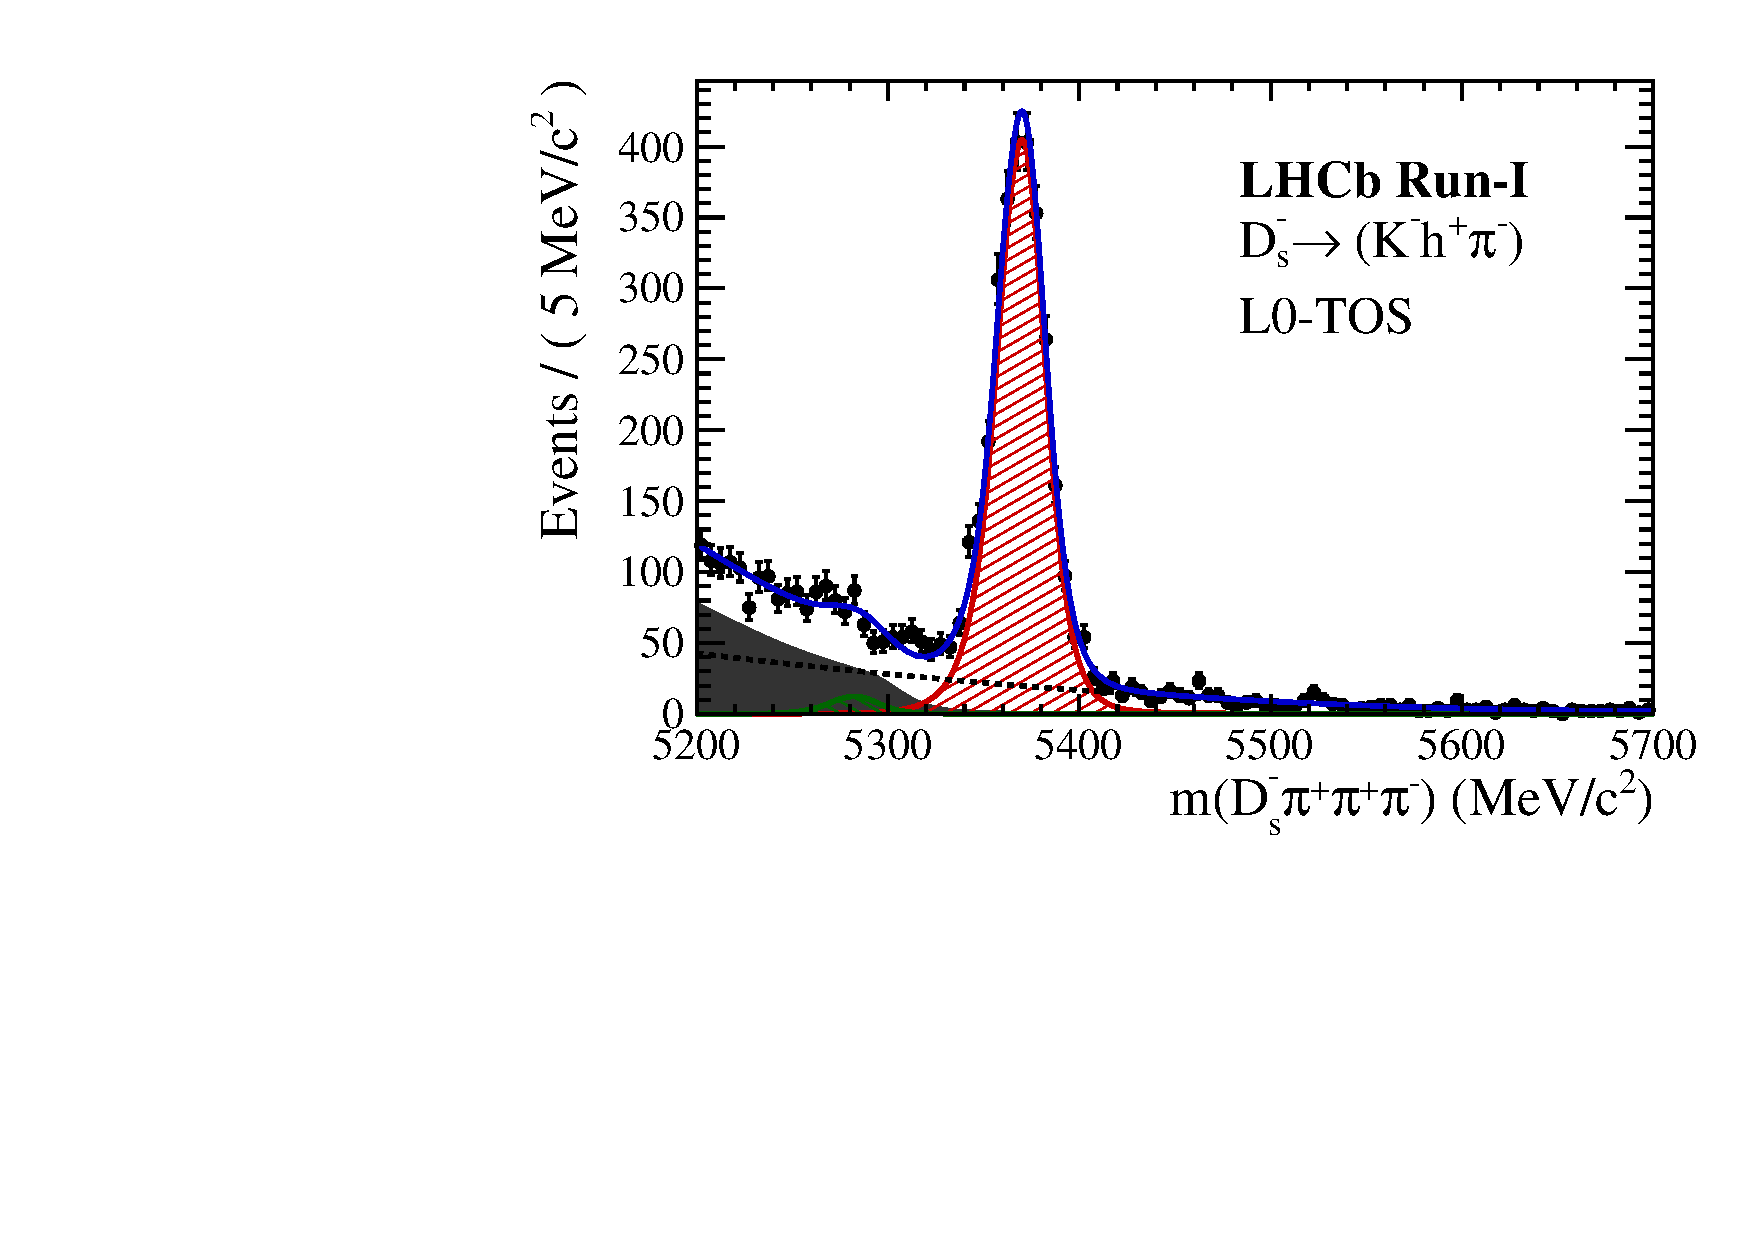
\includegraphics[height=!,width=0.4\textwidth]{figs/MassFit/norm_Run1_KKpi_NR_t0.pdf}
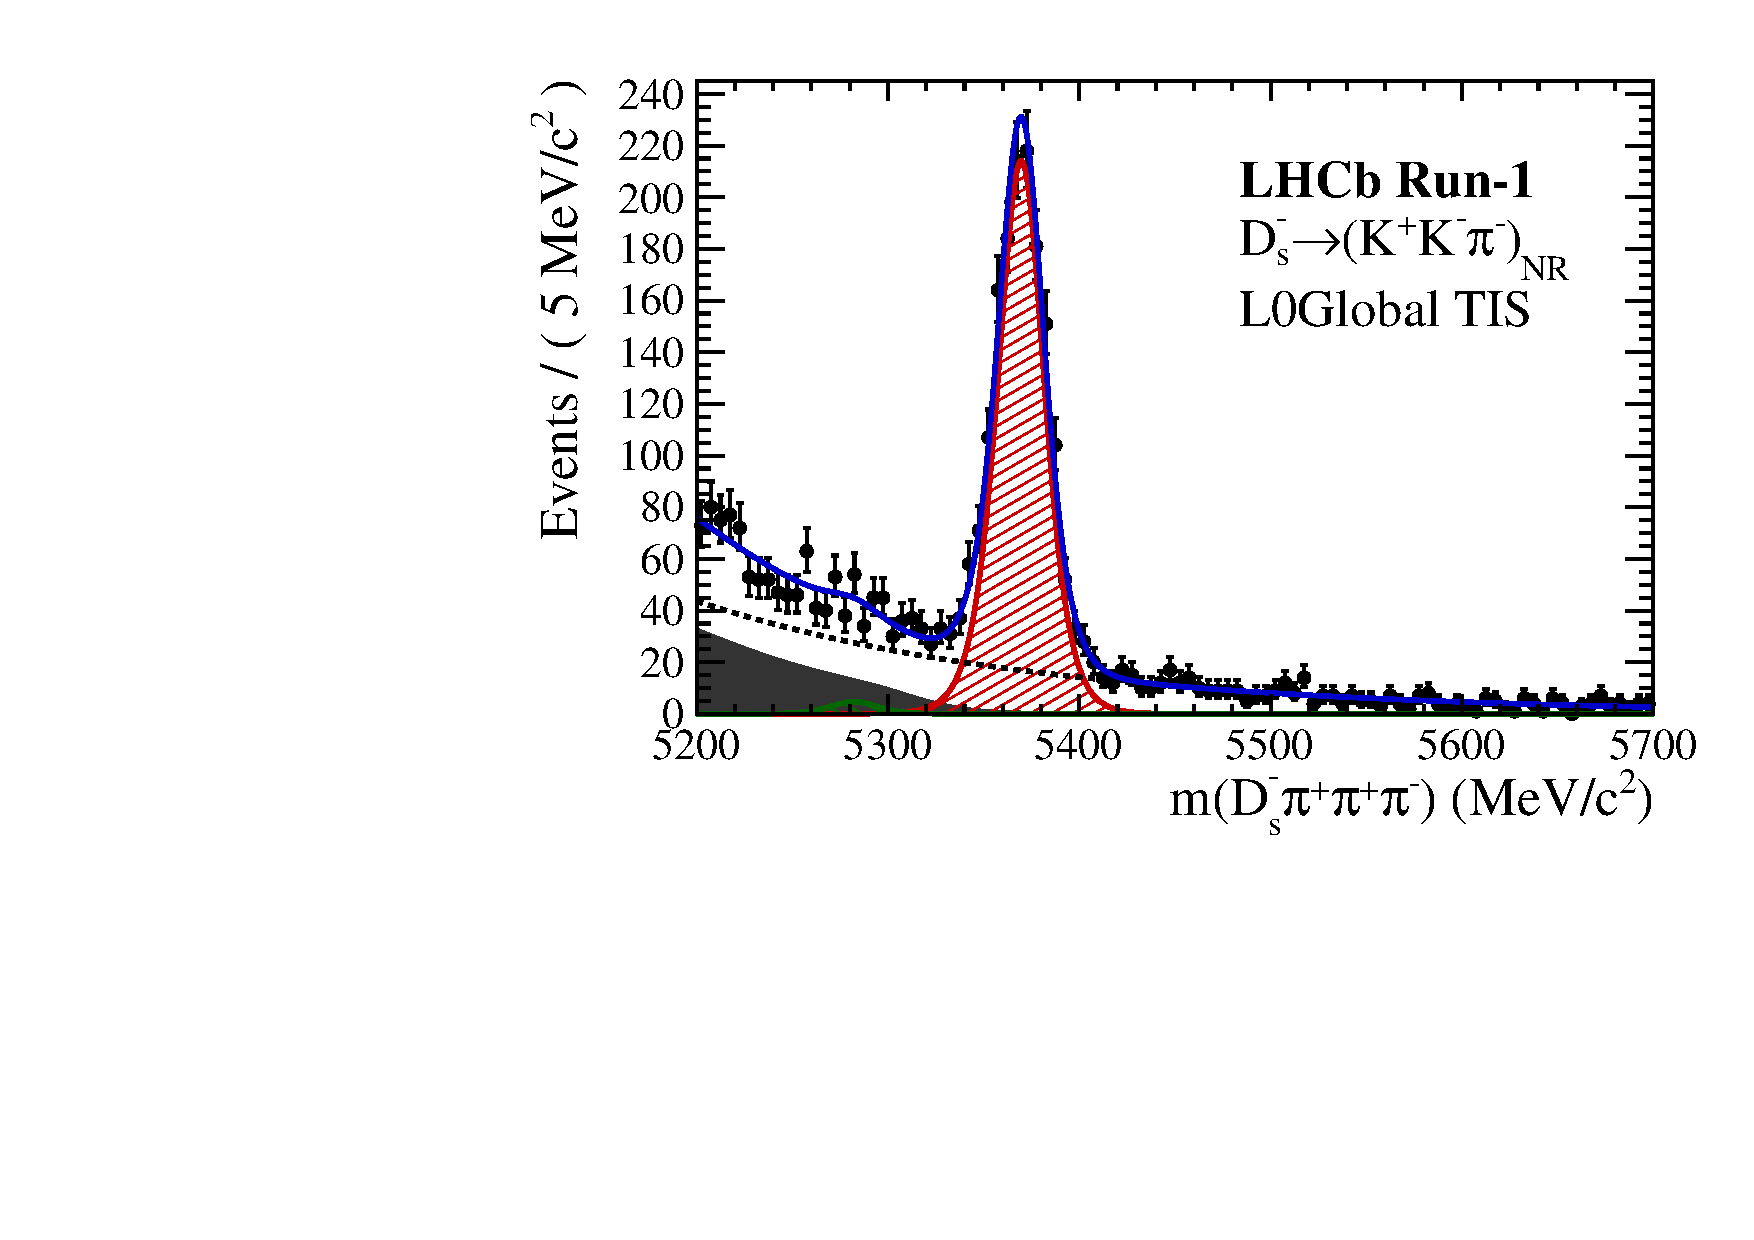
\includegraphics[height=!,width=0.4\textwidth]{figs/MassFit/norm_Run1_KKpi_NR_t1.pdf}

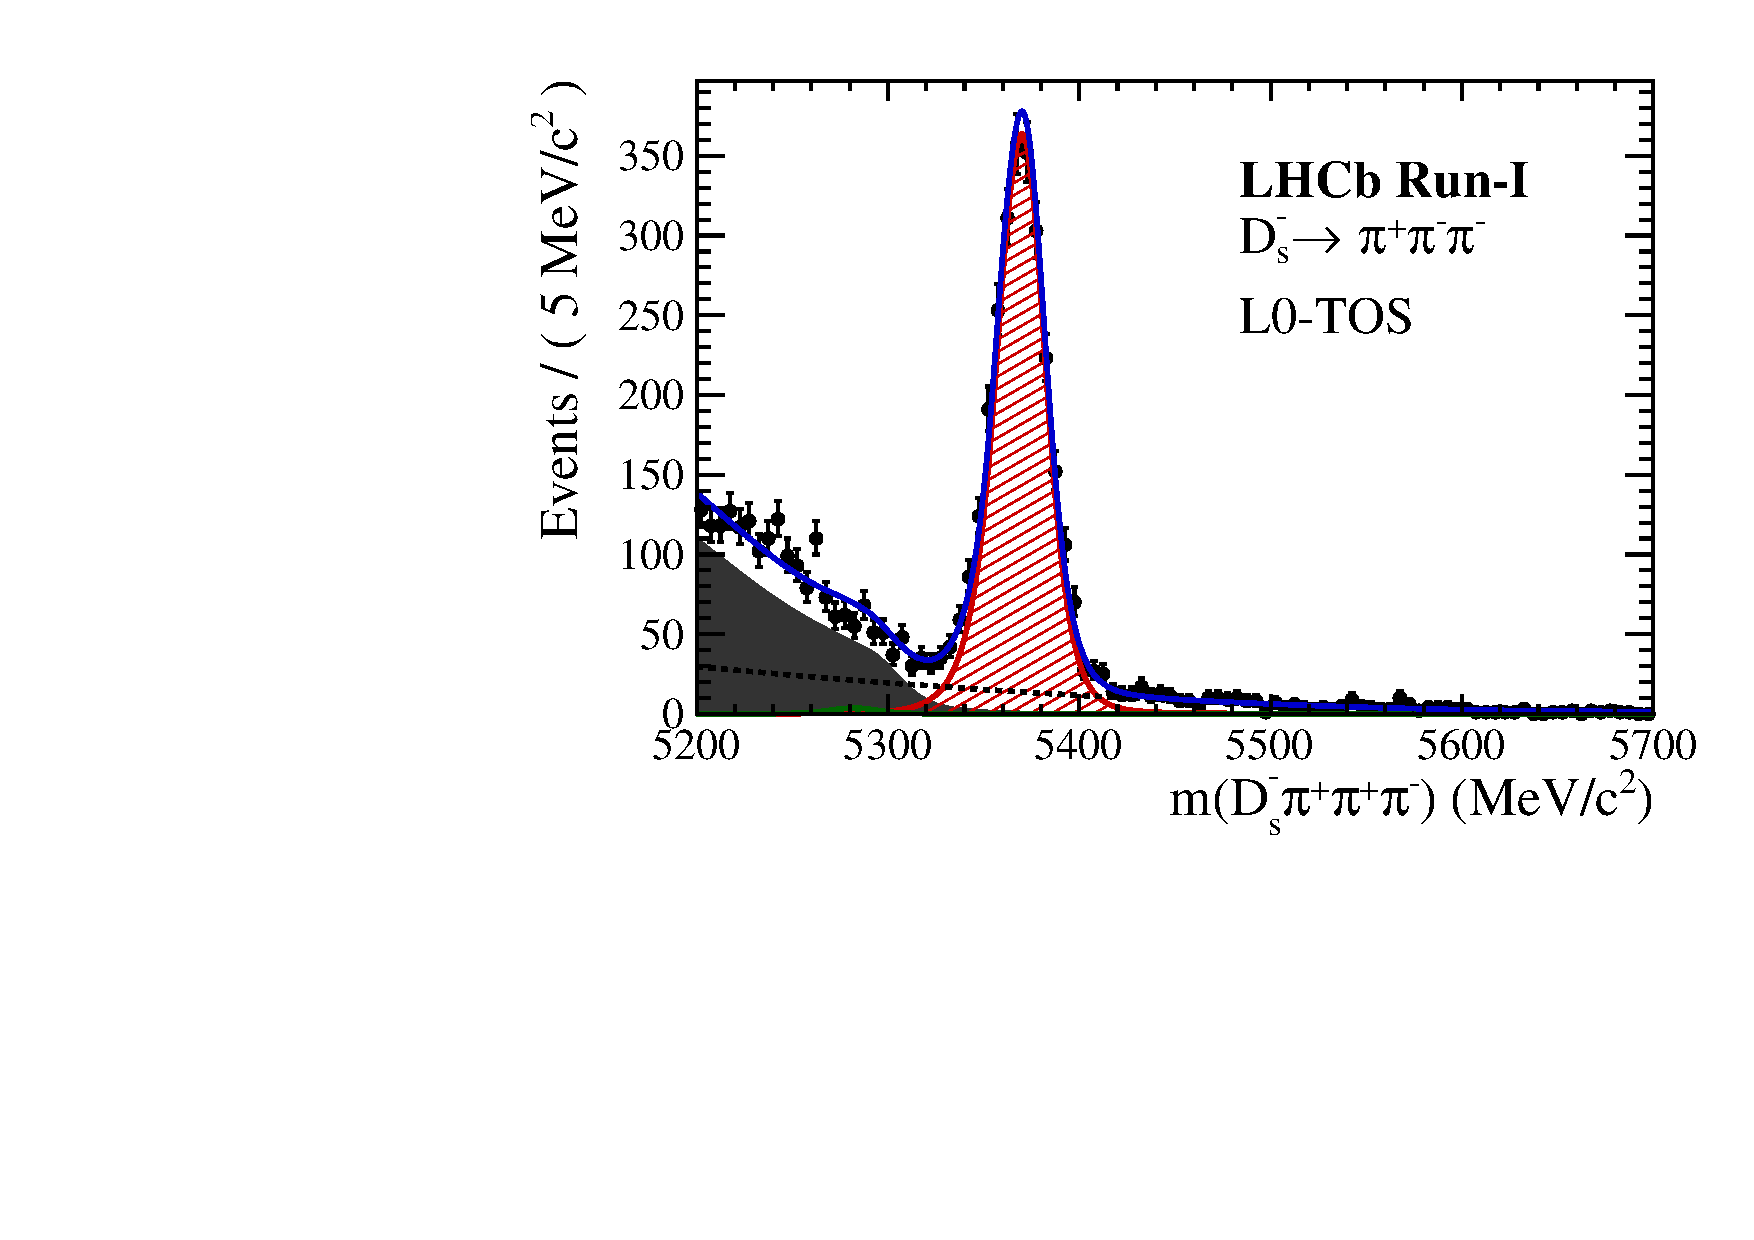
\includegraphics[height=!,width=0.4\textwidth]{figs/MassFit/norm_Run1_pipipi_t0.pdf}
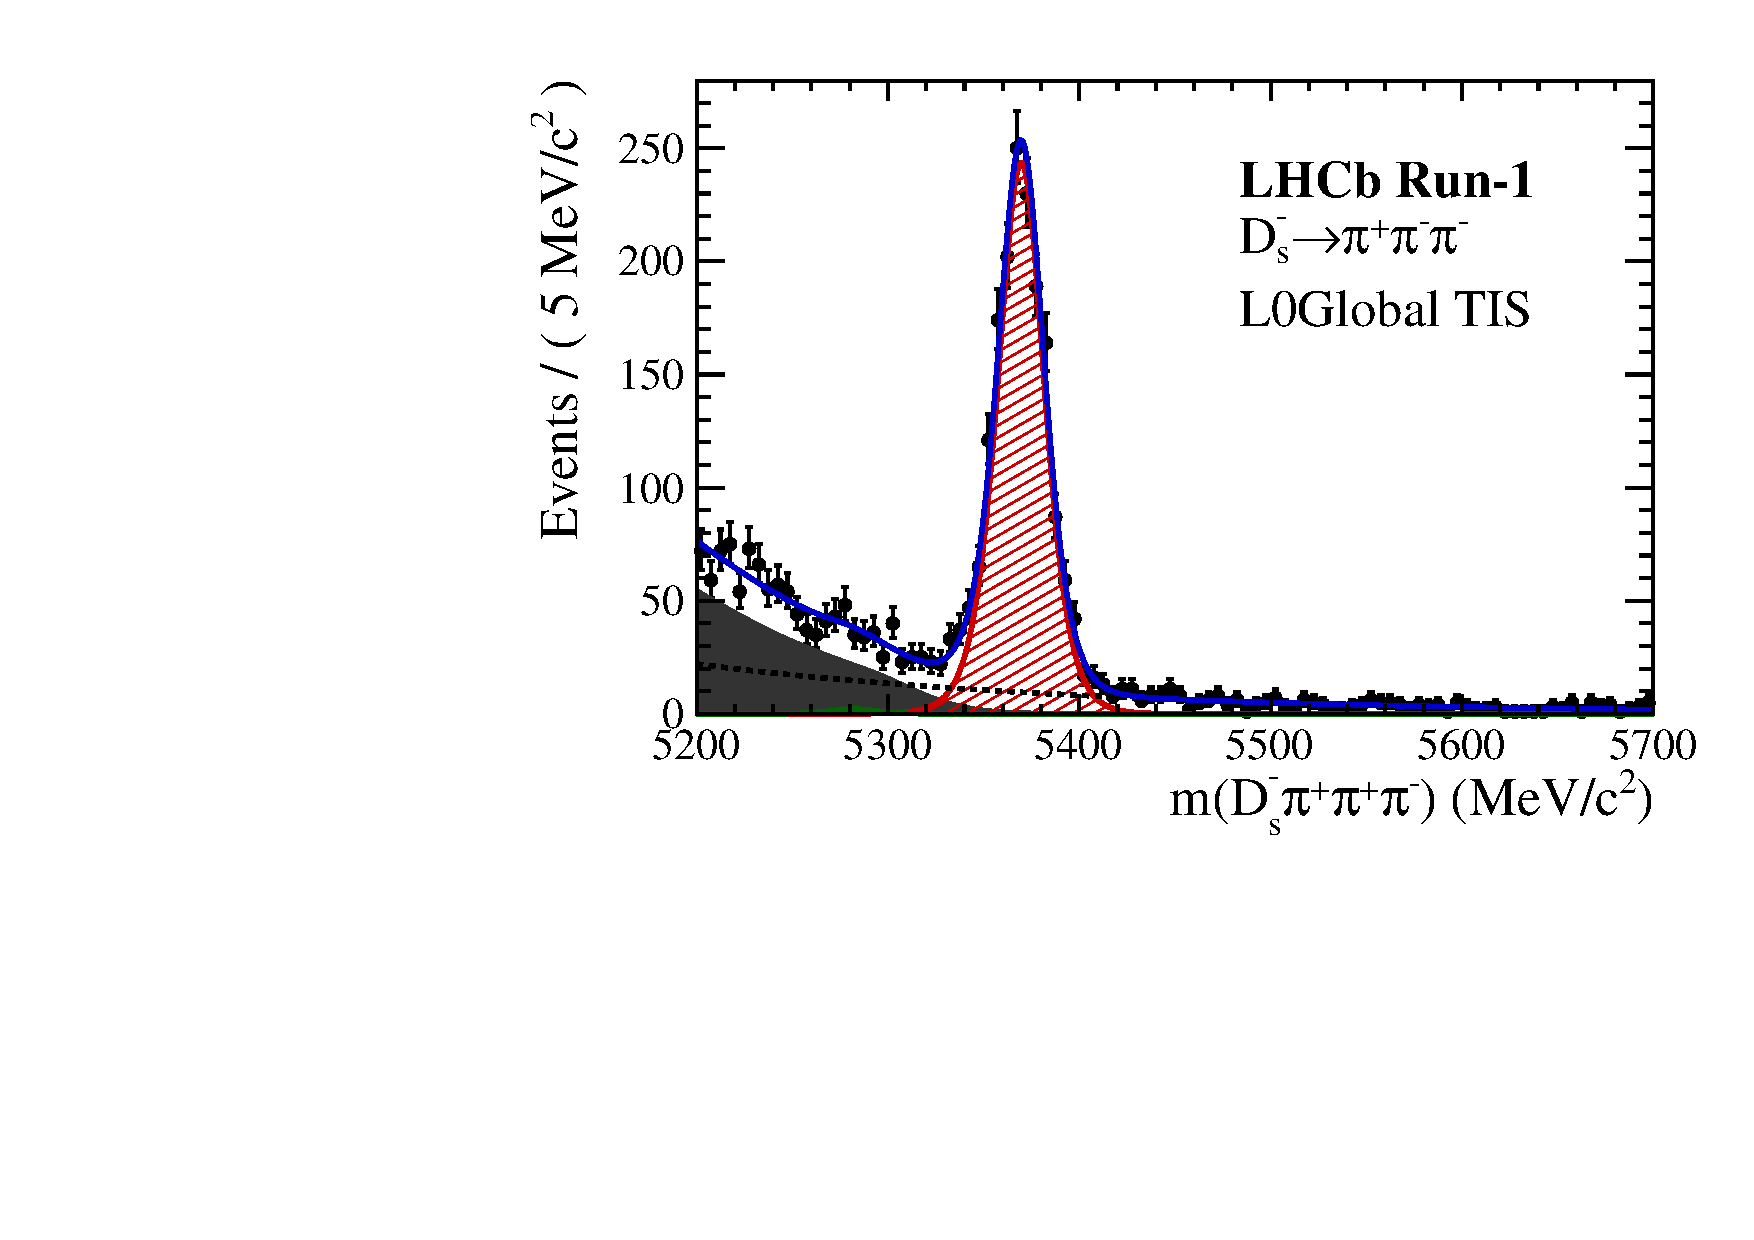
\includegraphics[height=!,width=0.4\textwidth]{figs/MassFit/norm_Run1_pipipi_t1.pdf}
\caption{Invariant mass distributions of $\Bs\to\Ds\pion\pion\pion$ candidates for Run-I data.}
\label{fig:massfits_norm_Run1}
\end{figure}

\clearpage

\begin{figure}[h]
\centering
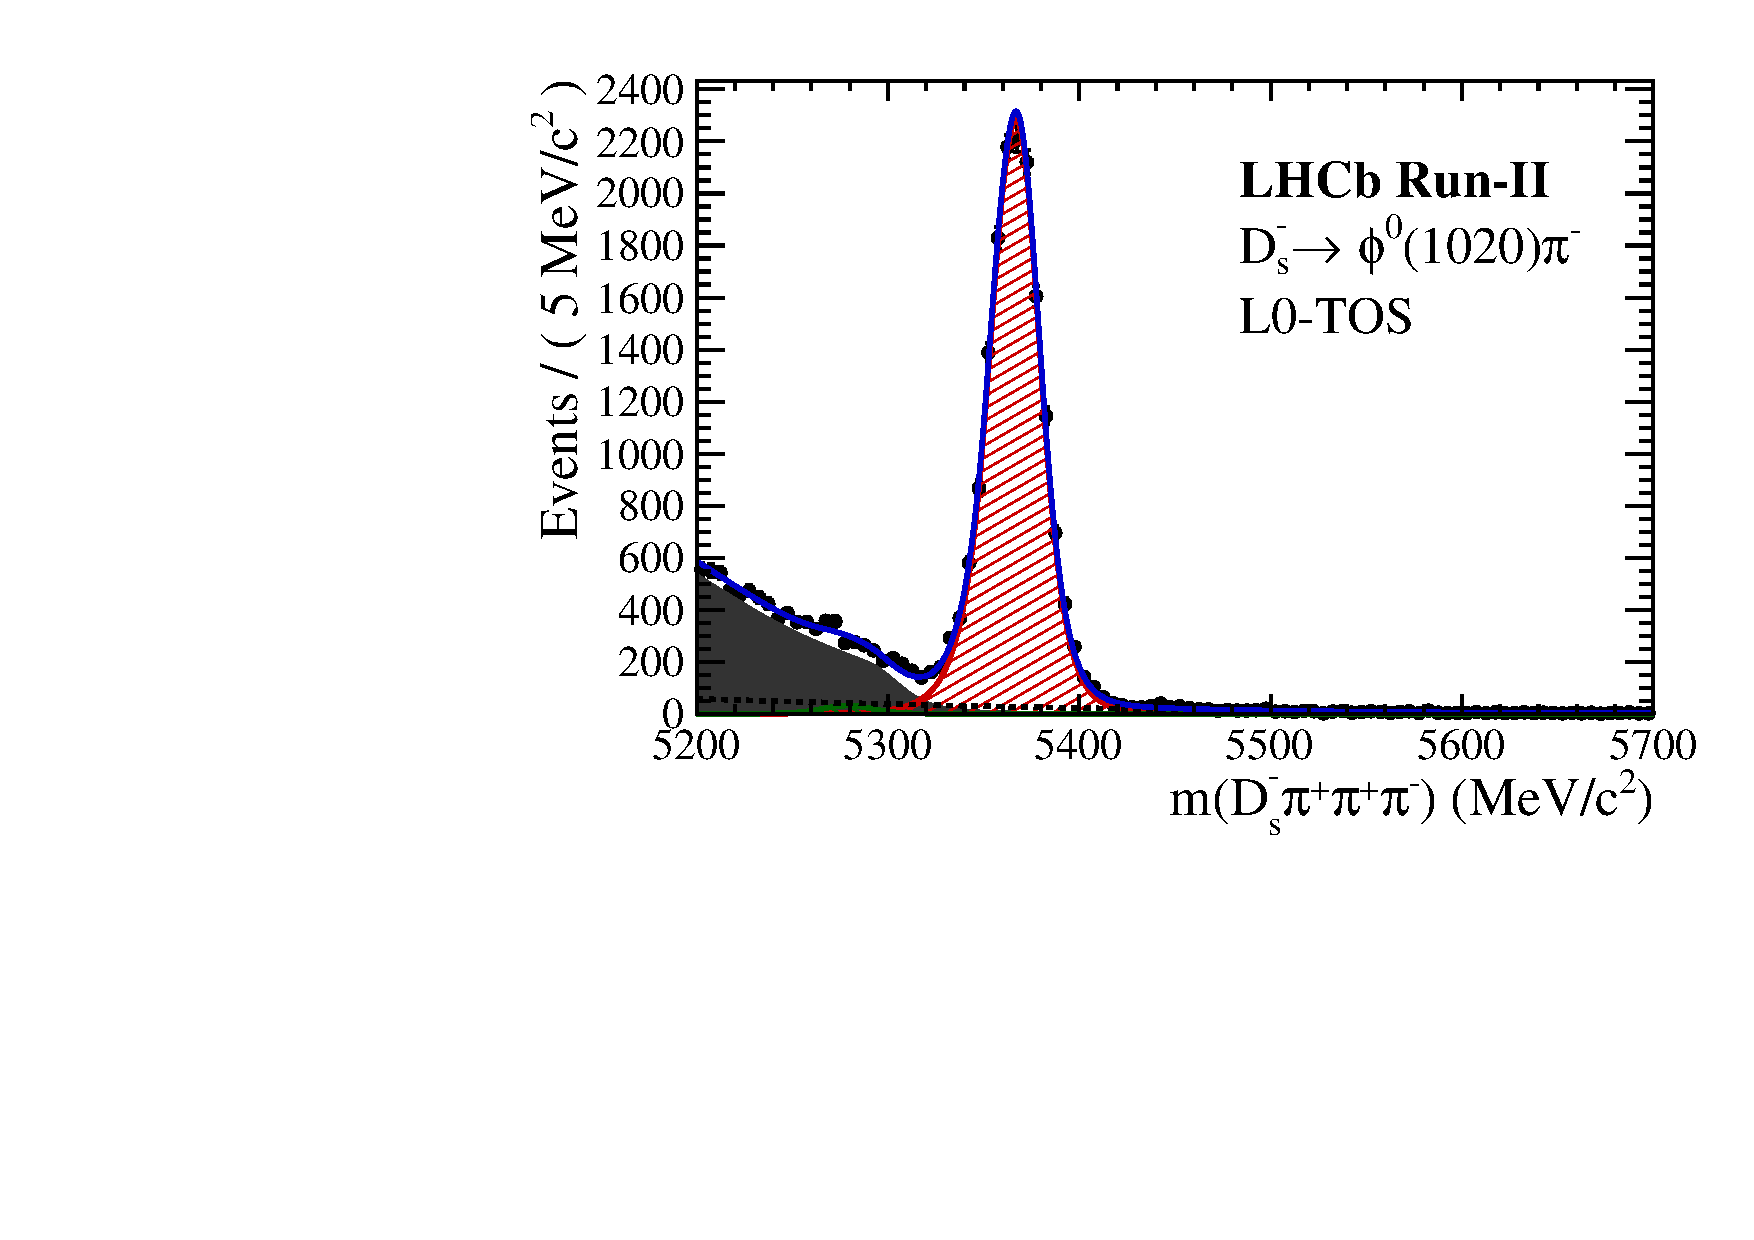
\includegraphics[height=!,width=0.4\textwidth]{figs/MassFit/norm_Run2_phipi_t0.pdf}
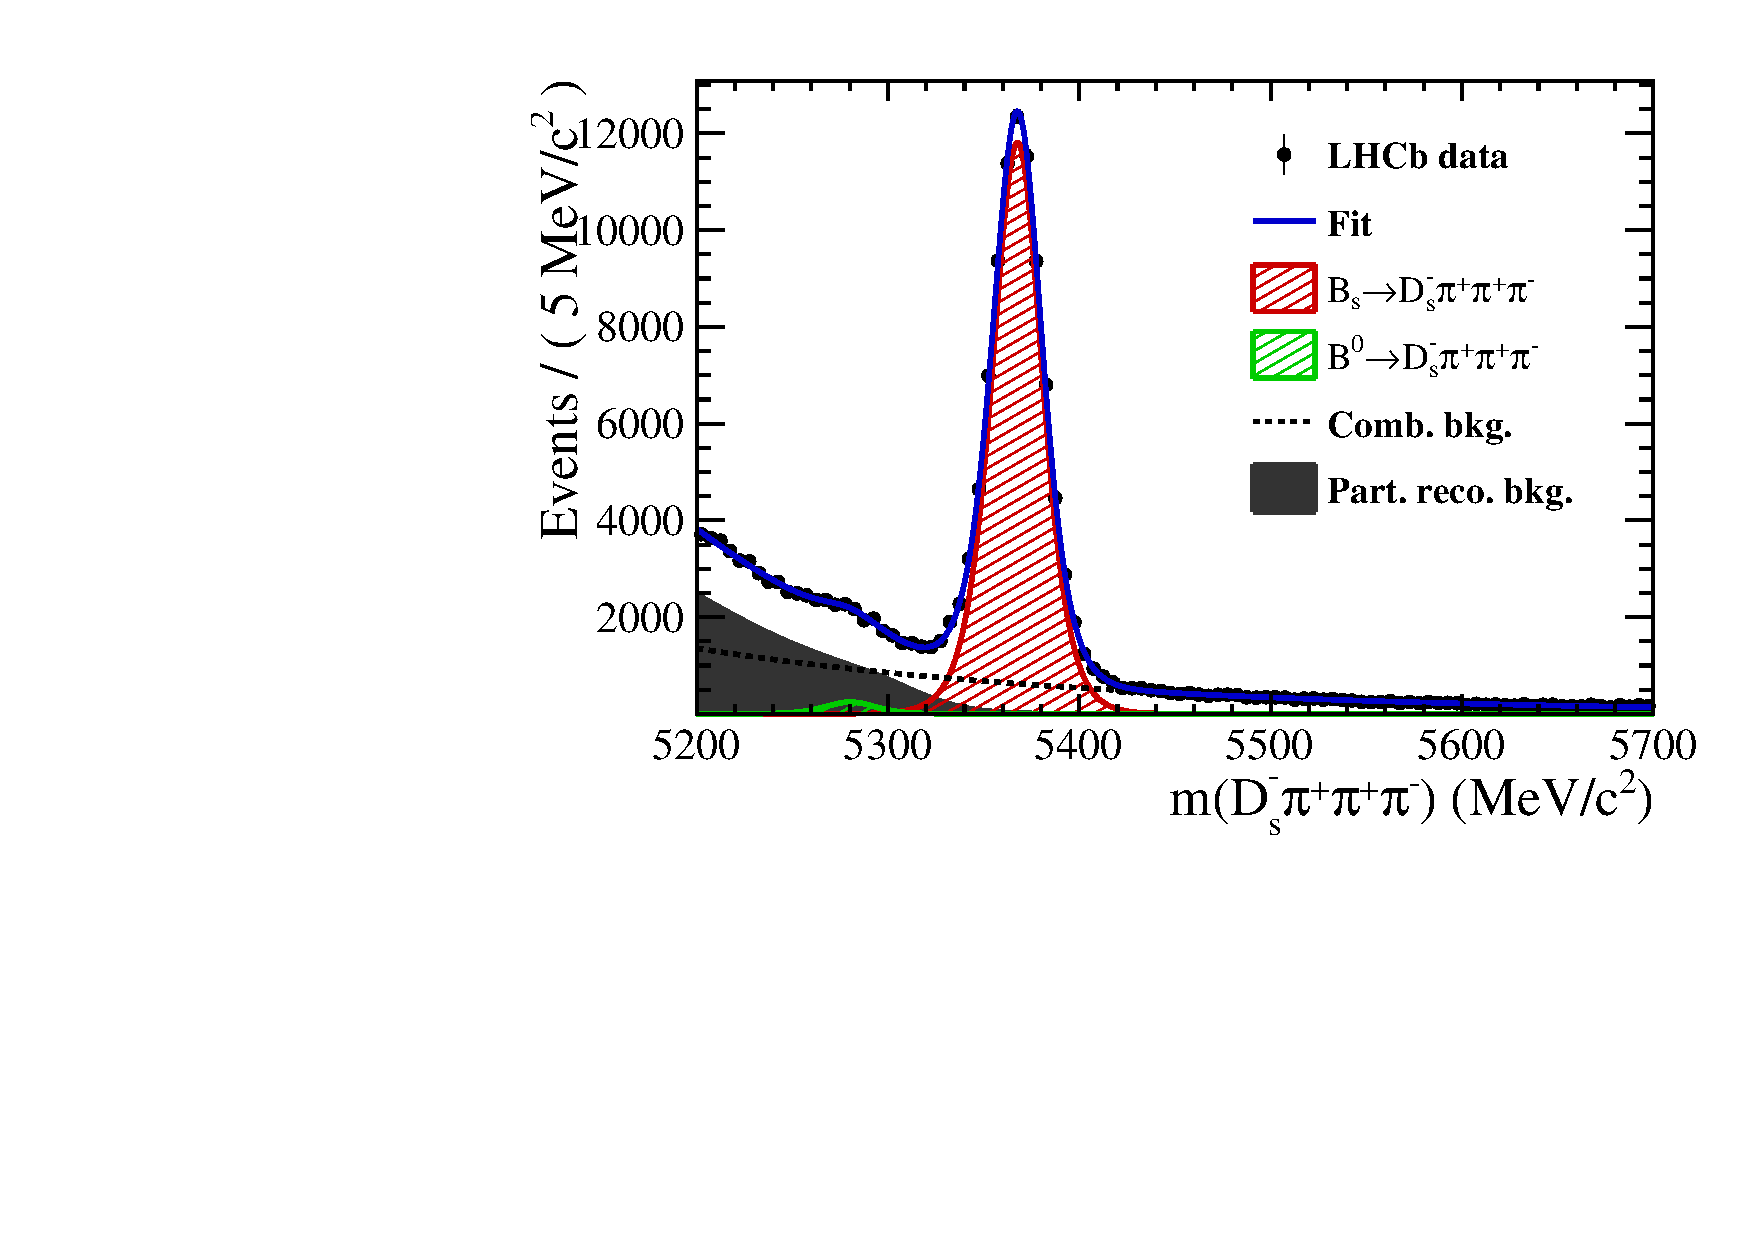
\includegraphics[height=!,width=0.4\textwidth]{figs/MassFit/norm_Run2_phipi_t1.pdf}

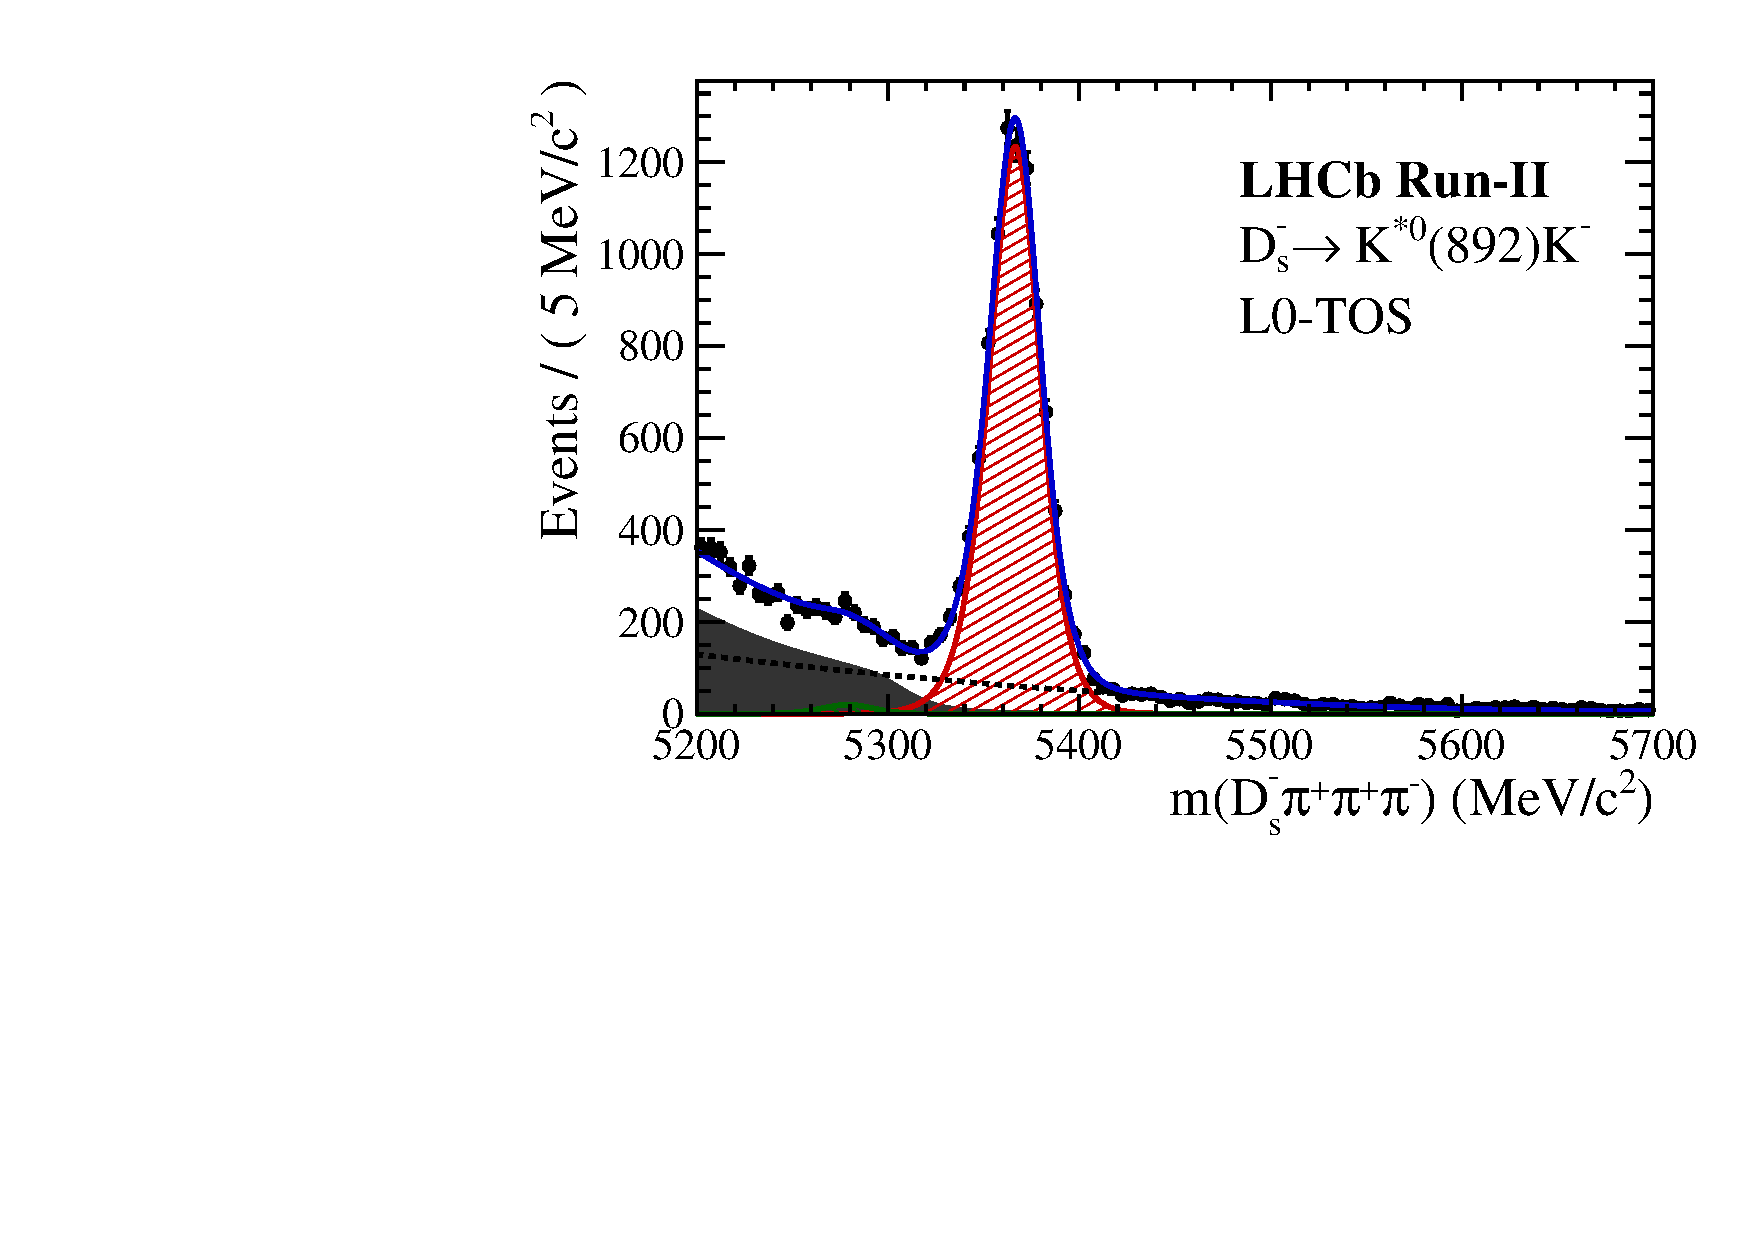
\includegraphics[height=!,width=0.4\textwidth]{figs/MassFit/norm_Run2_KsK_t0.pdf}
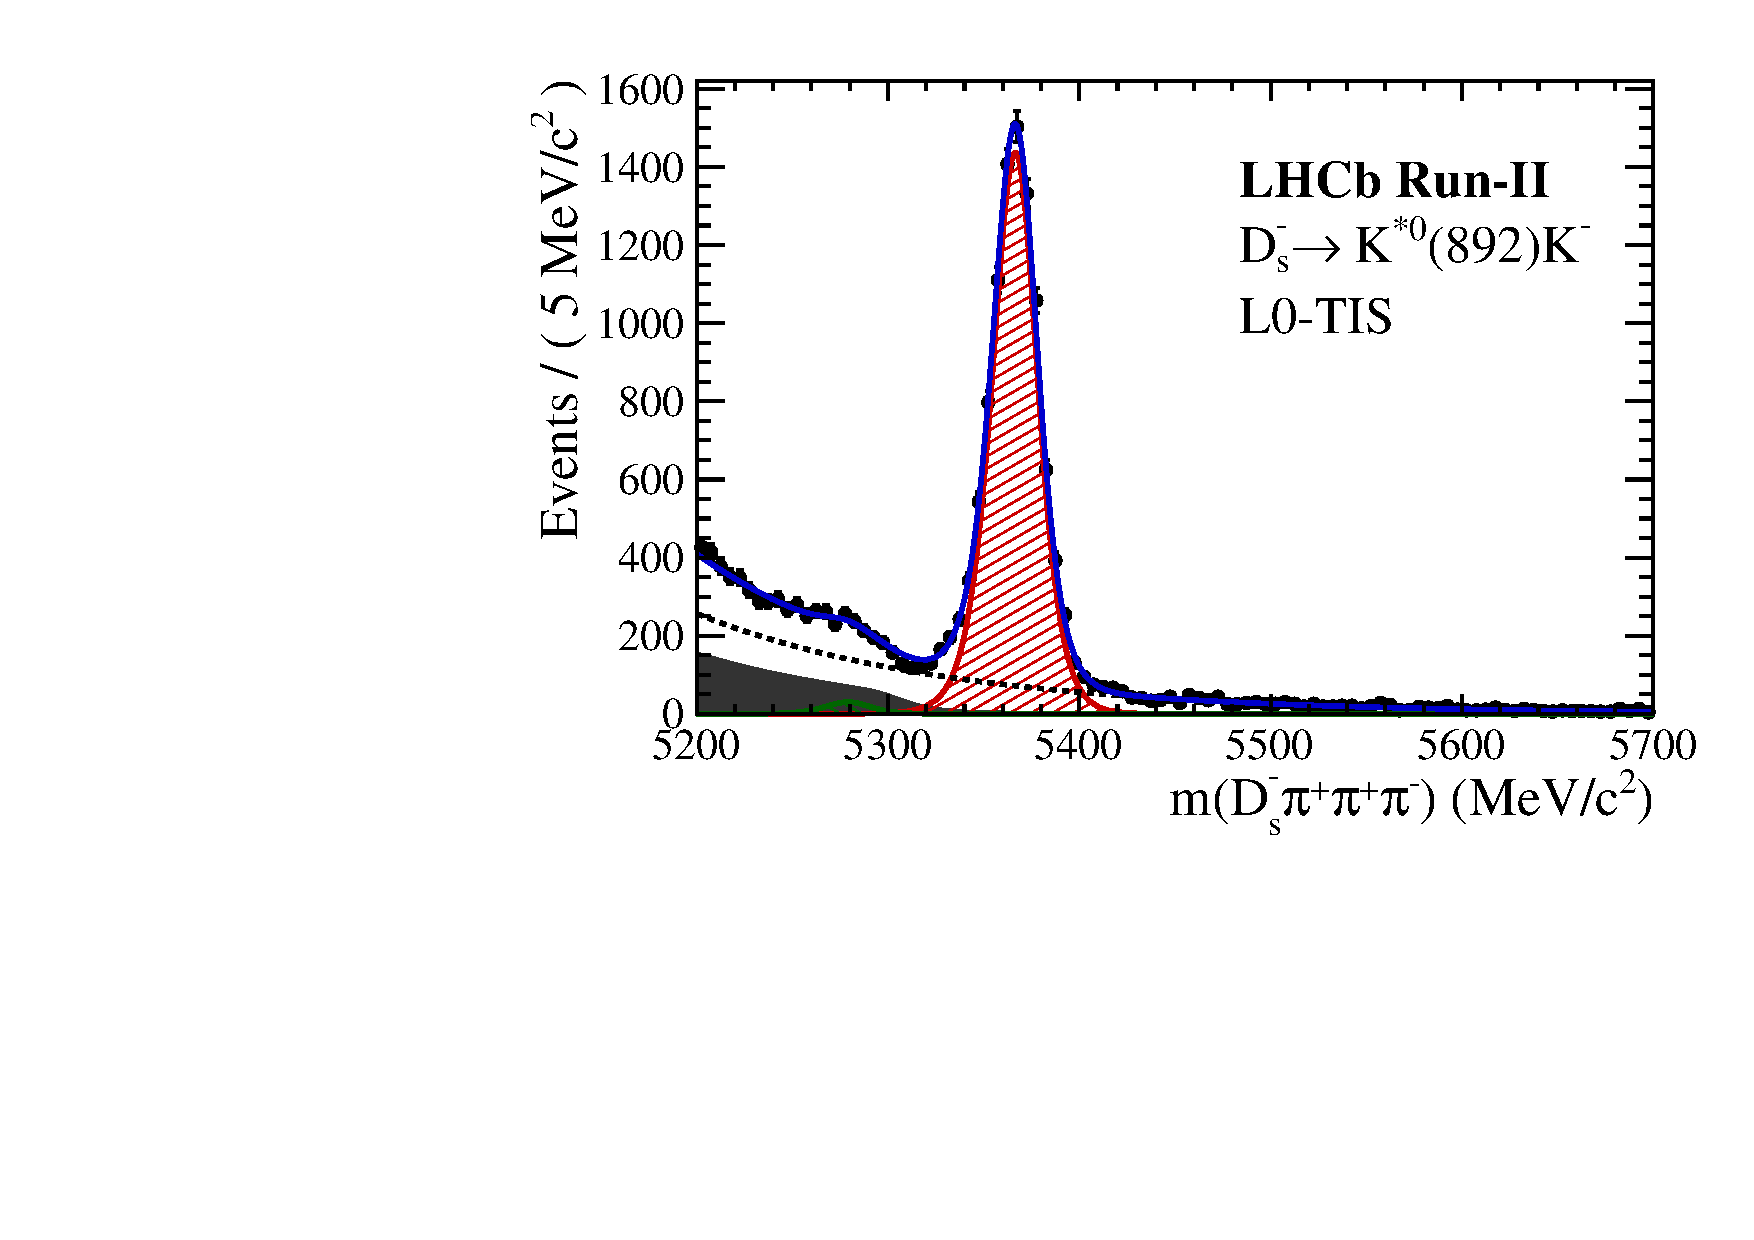
\includegraphics[height=!,width=0.4\textwidth]{figs/MassFit/norm_Run2_KsK_t1.pdf}

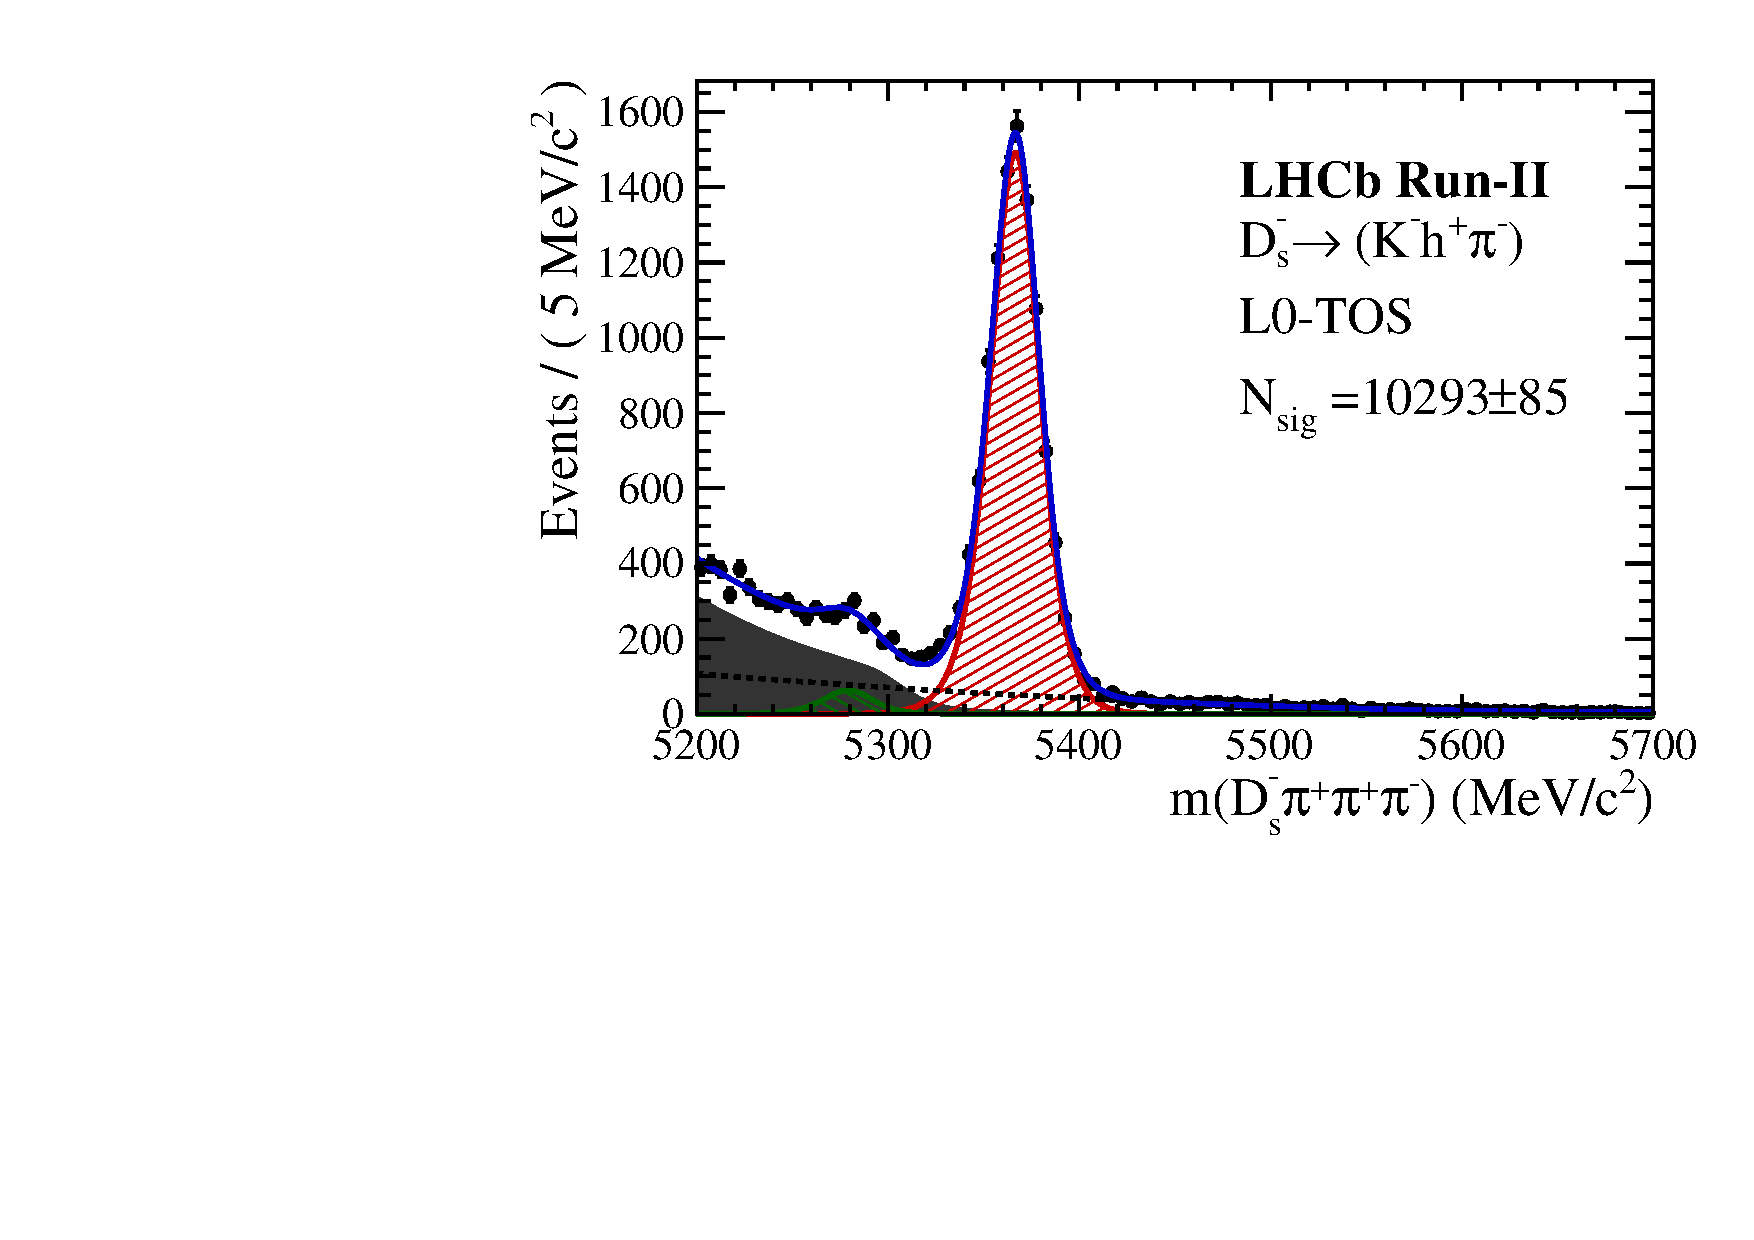
\includegraphics[height=!,width=0.4\textwidth]{figs/MassFit/norm_Run2_KKpi_NR_t0.pdf}
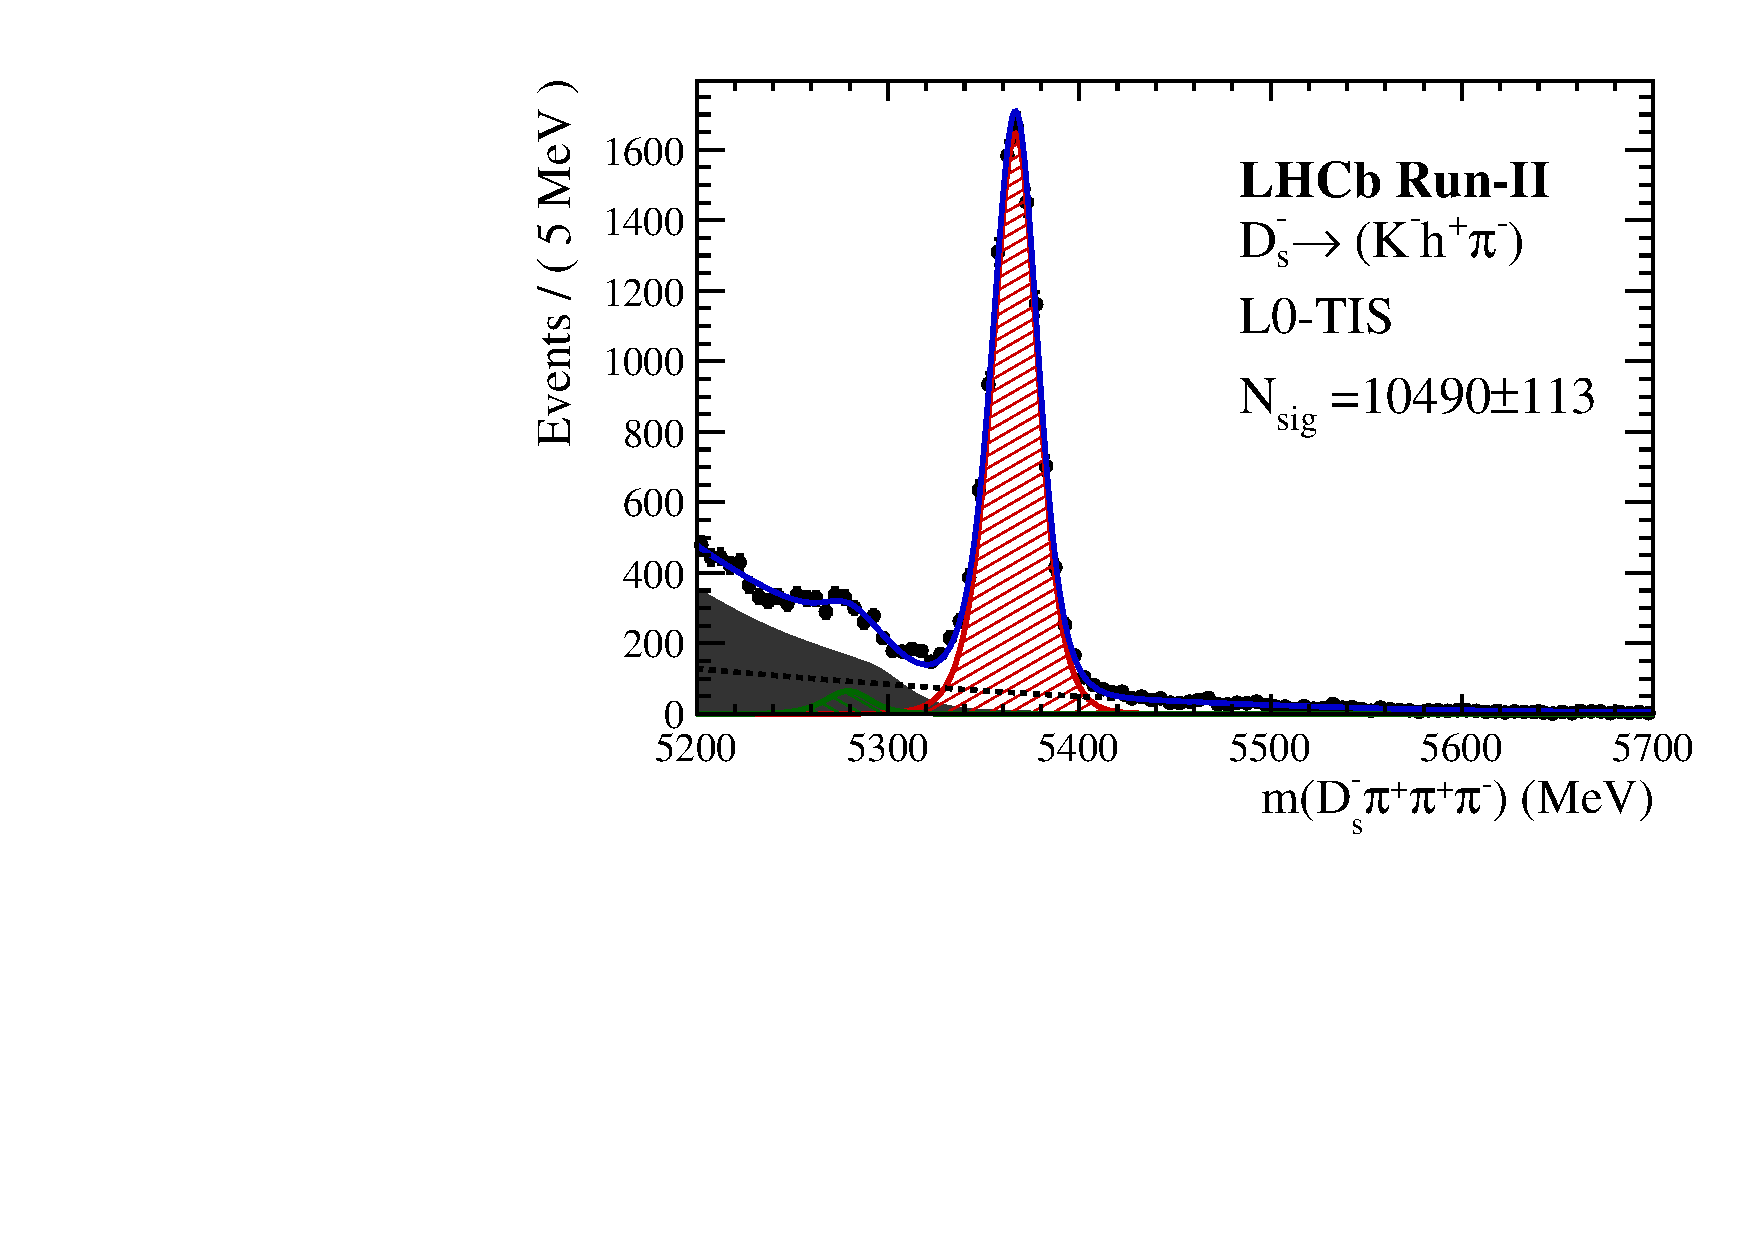
\includegraphics[height=!,width=0.4\textwidth]{figs/MassFit/norm_Run2_KKpi_NR_t1.pdf}

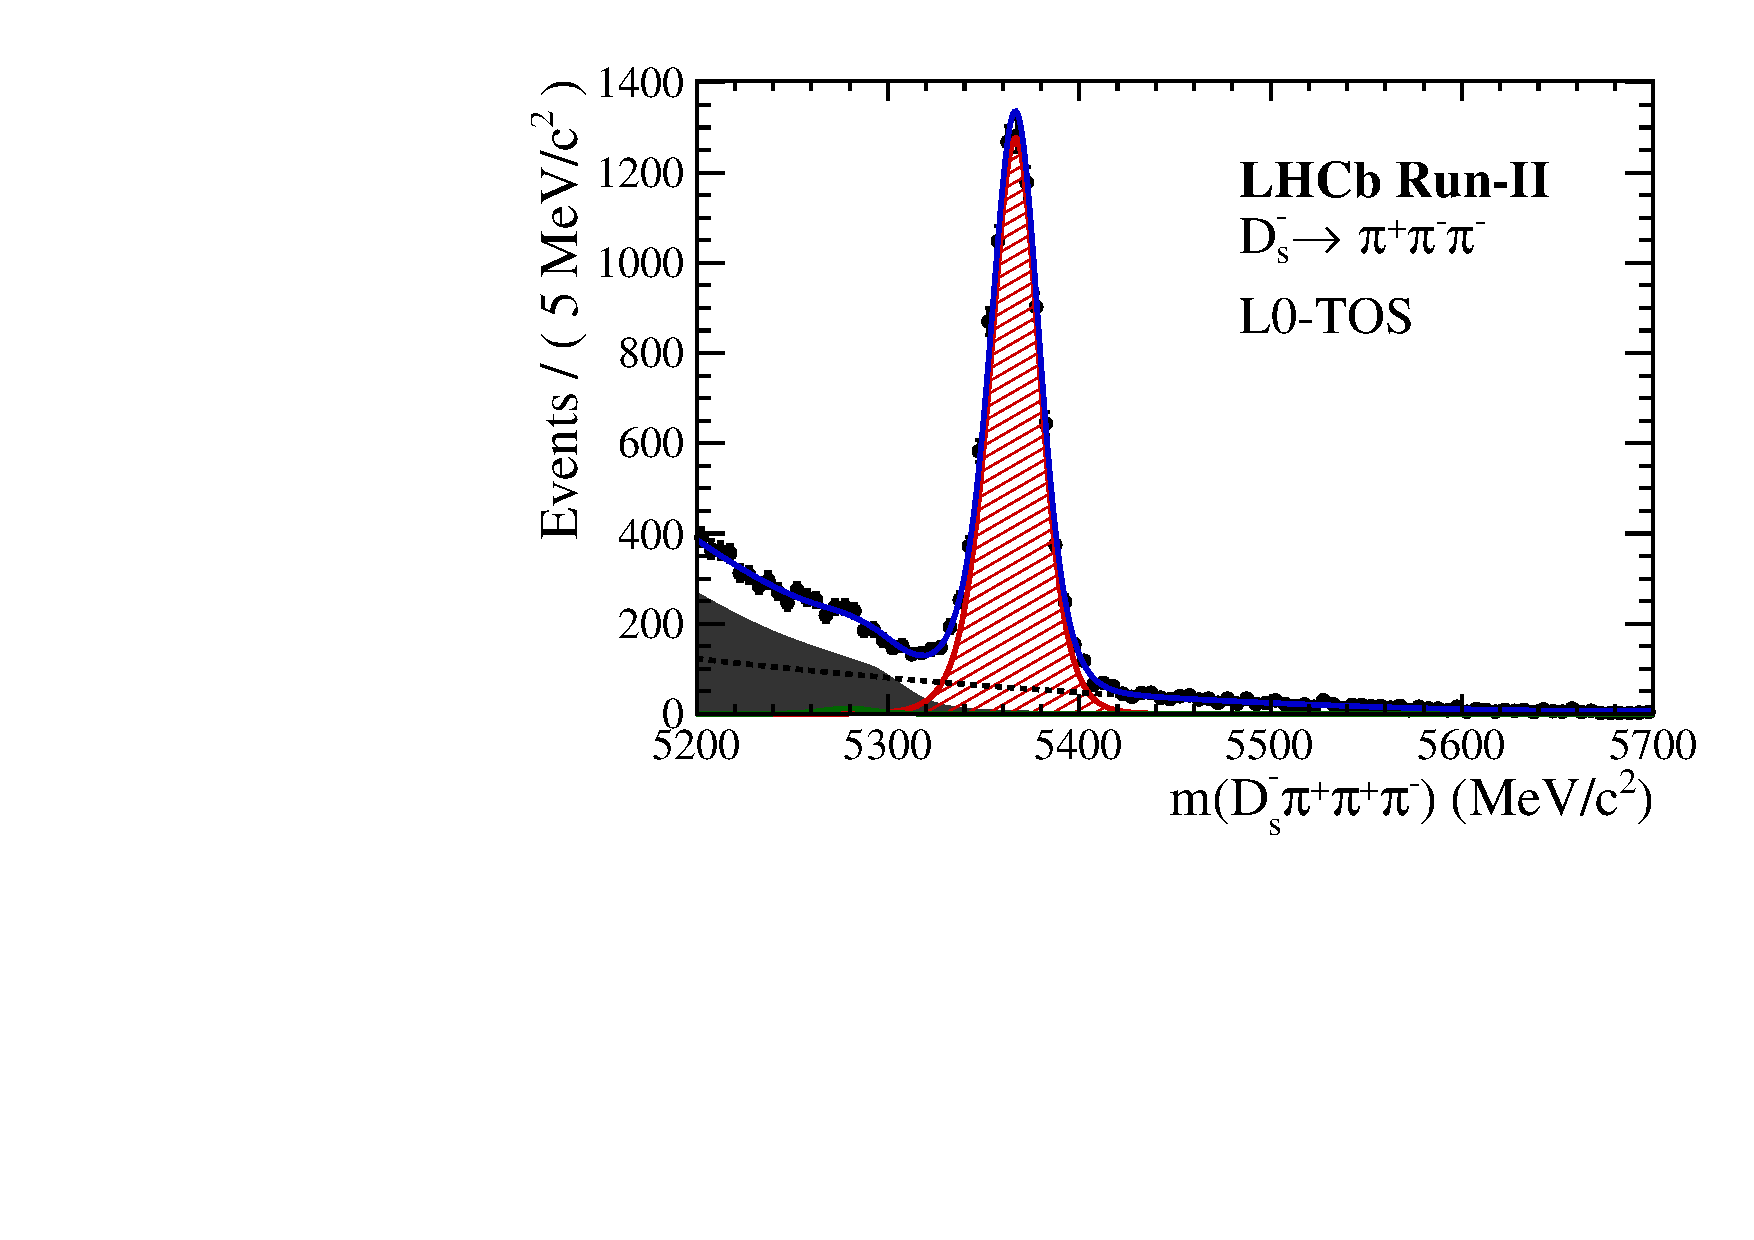
\includegraphics[height=!,width=0.4\textwidth]{figs/MassFit/norm_Run2_pipipi_t0.pdf}
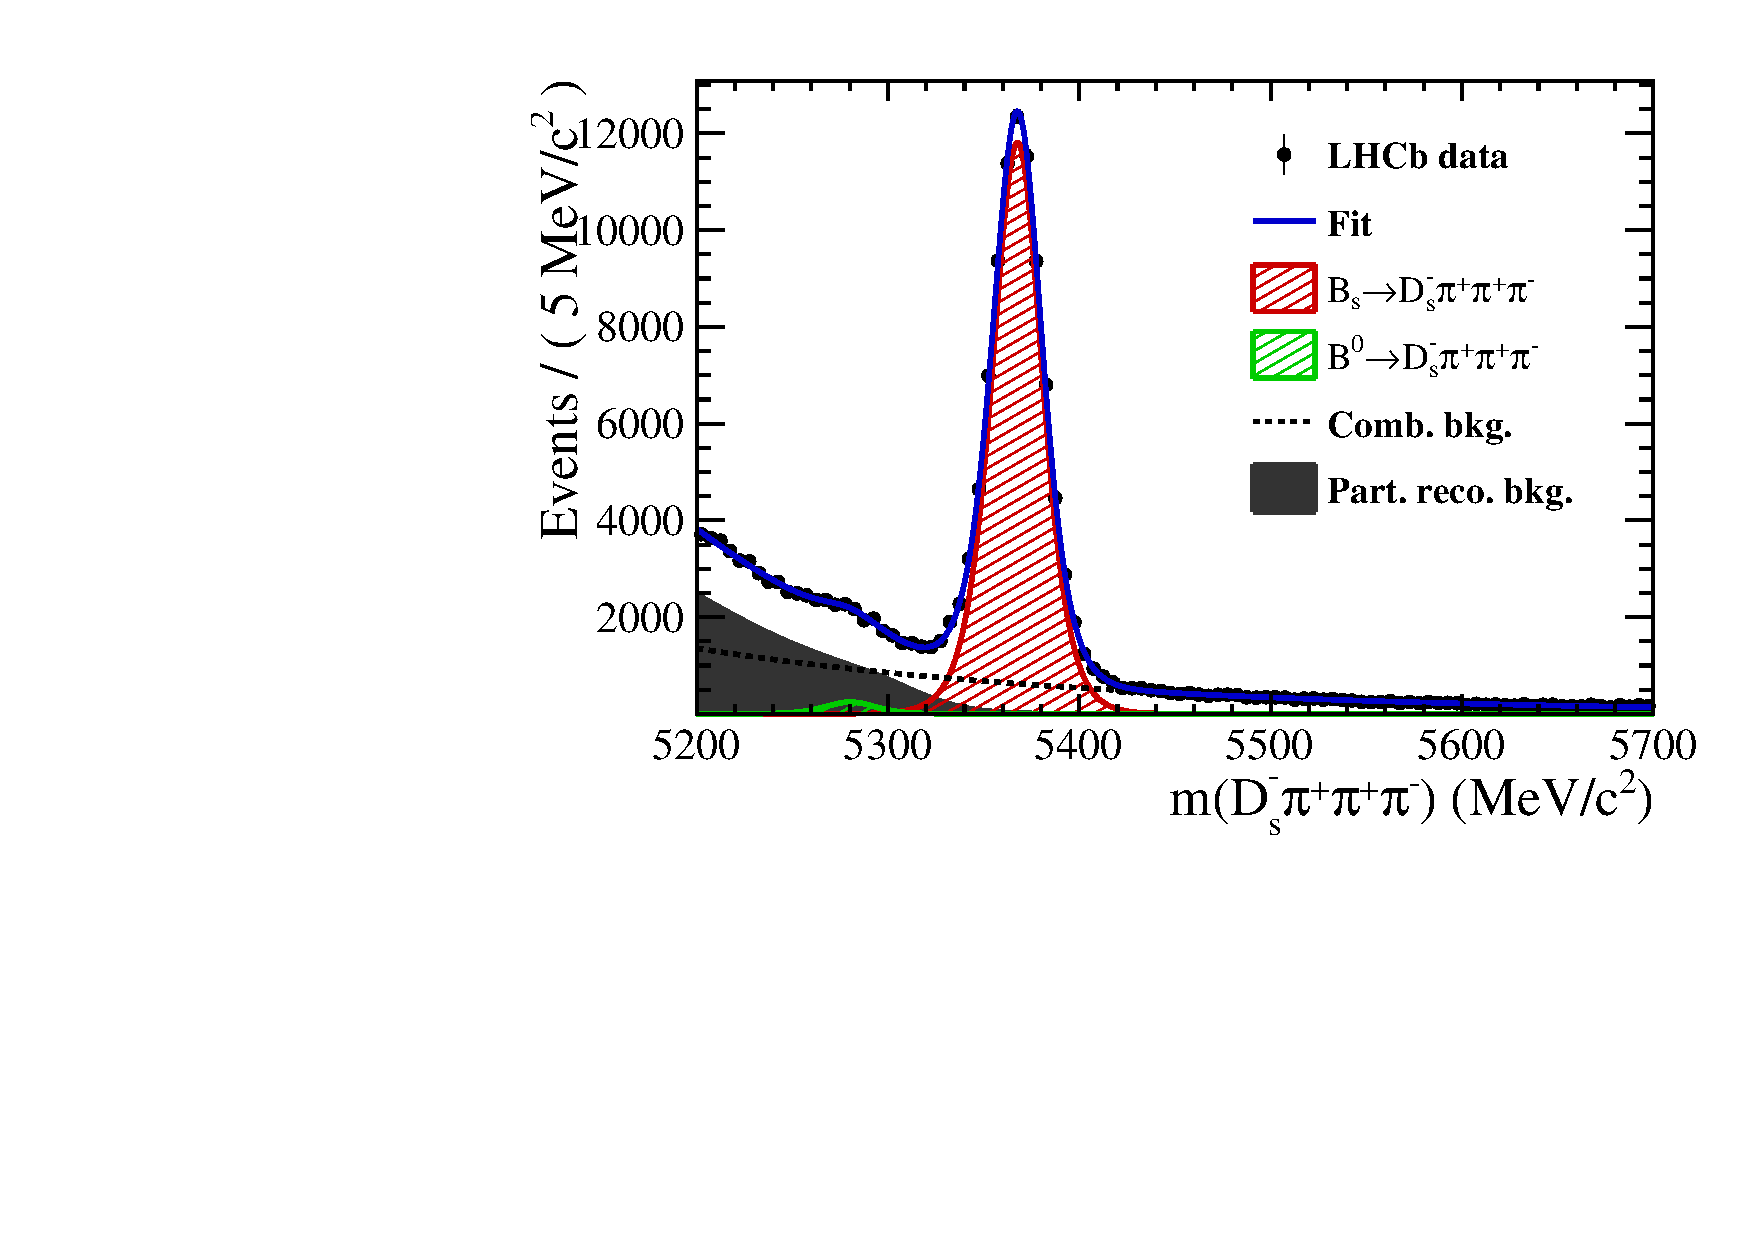
\includegraphics[height=!,width=0.4\textwidth]{figs/MassFit/norm_Run2_pipipi_t1.pdf}
\caption{Invariant mass distributions of $\Bs\to\Ds\pion\pion\pion$ candidates for Run-II data.}
\label{fig:massfits_norm_Run2}
\end{figure}

\clearpage

\begin{figure}[h]
\centering
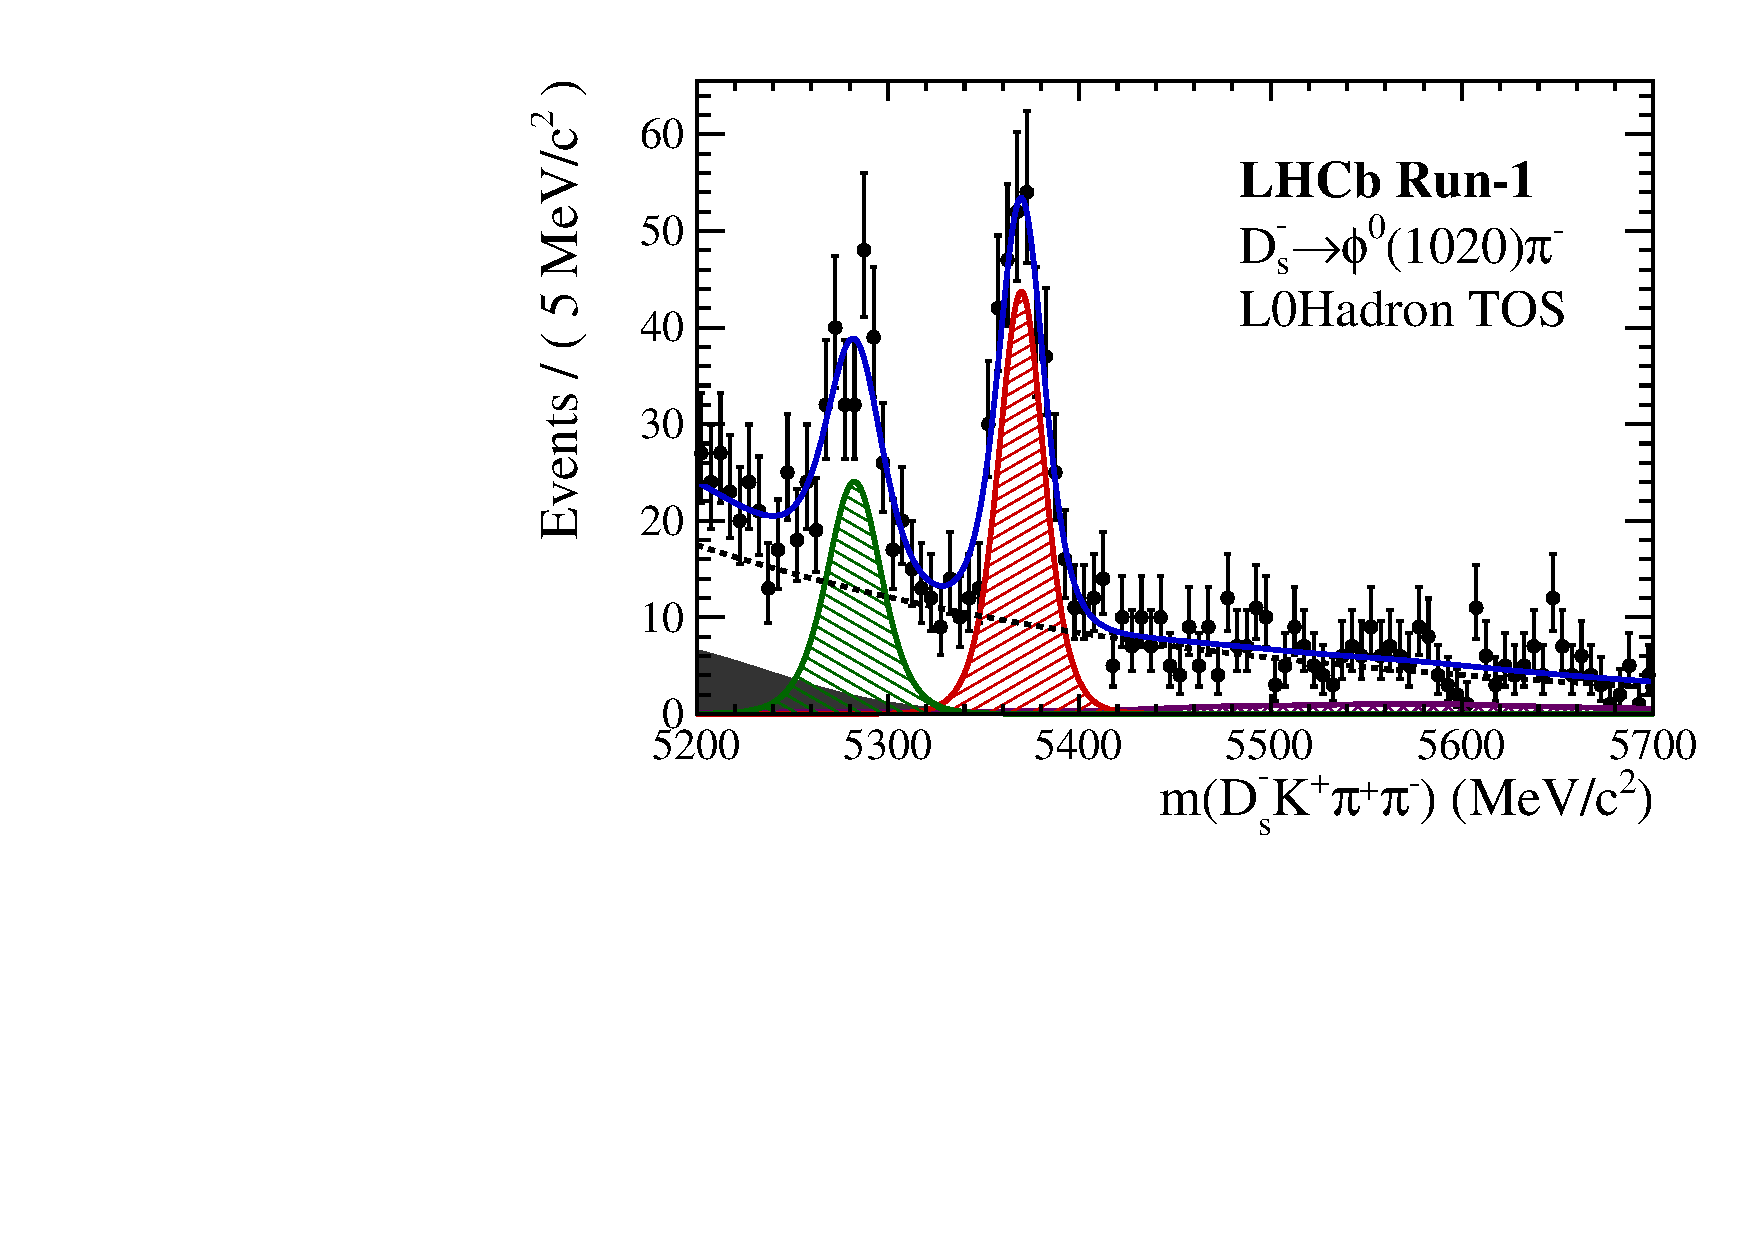
\includegraphics[height=!,width=0.4\textwidth]{figs/MassFit/signal_Run1_phipi_t0.pdf}
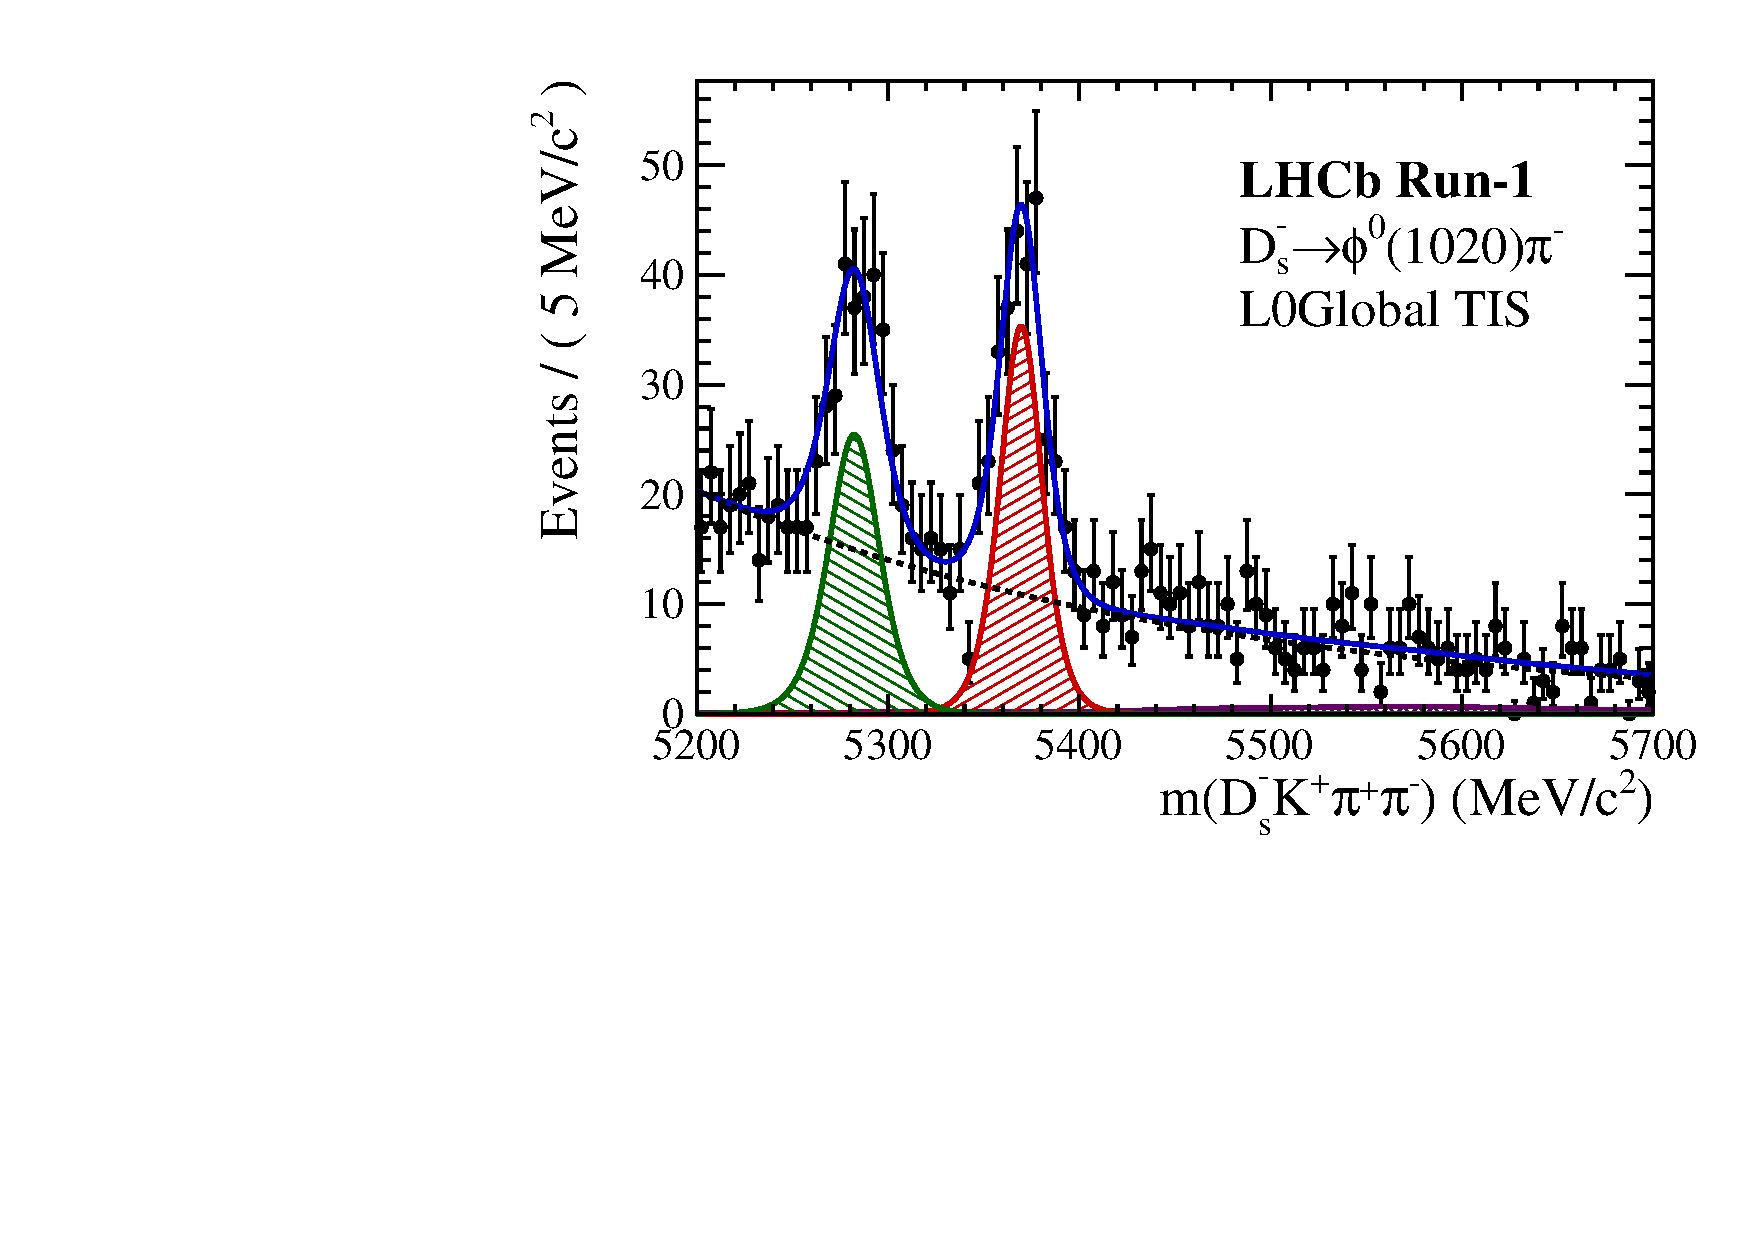
\includegraphics[height=!,width=0.4\textwidth]{figs/MassFit/signal_Run1_phipi_t1.pdf}

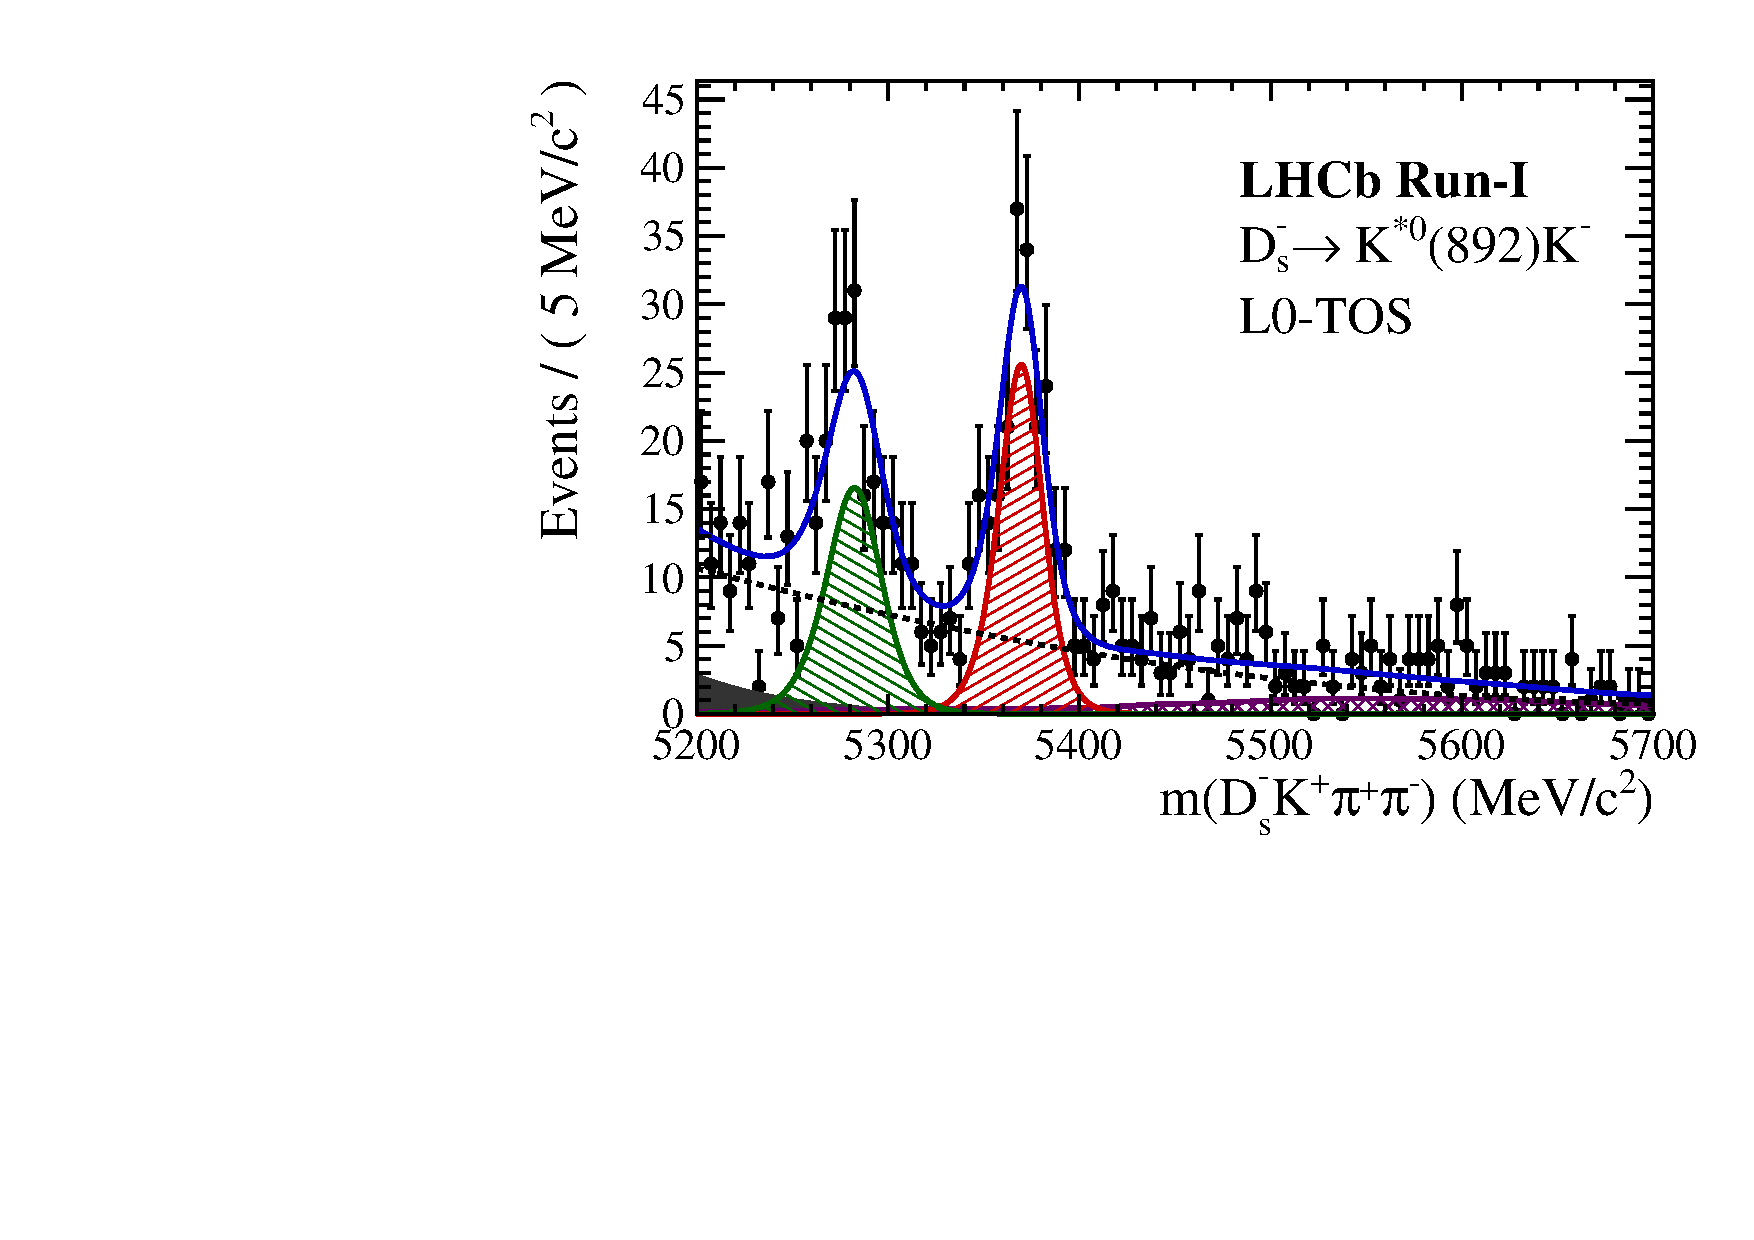
\includegraphics[height=!,width=0.4\textwidth]{figs/MassFit/signal_Run1_KsK_t0.pdf}
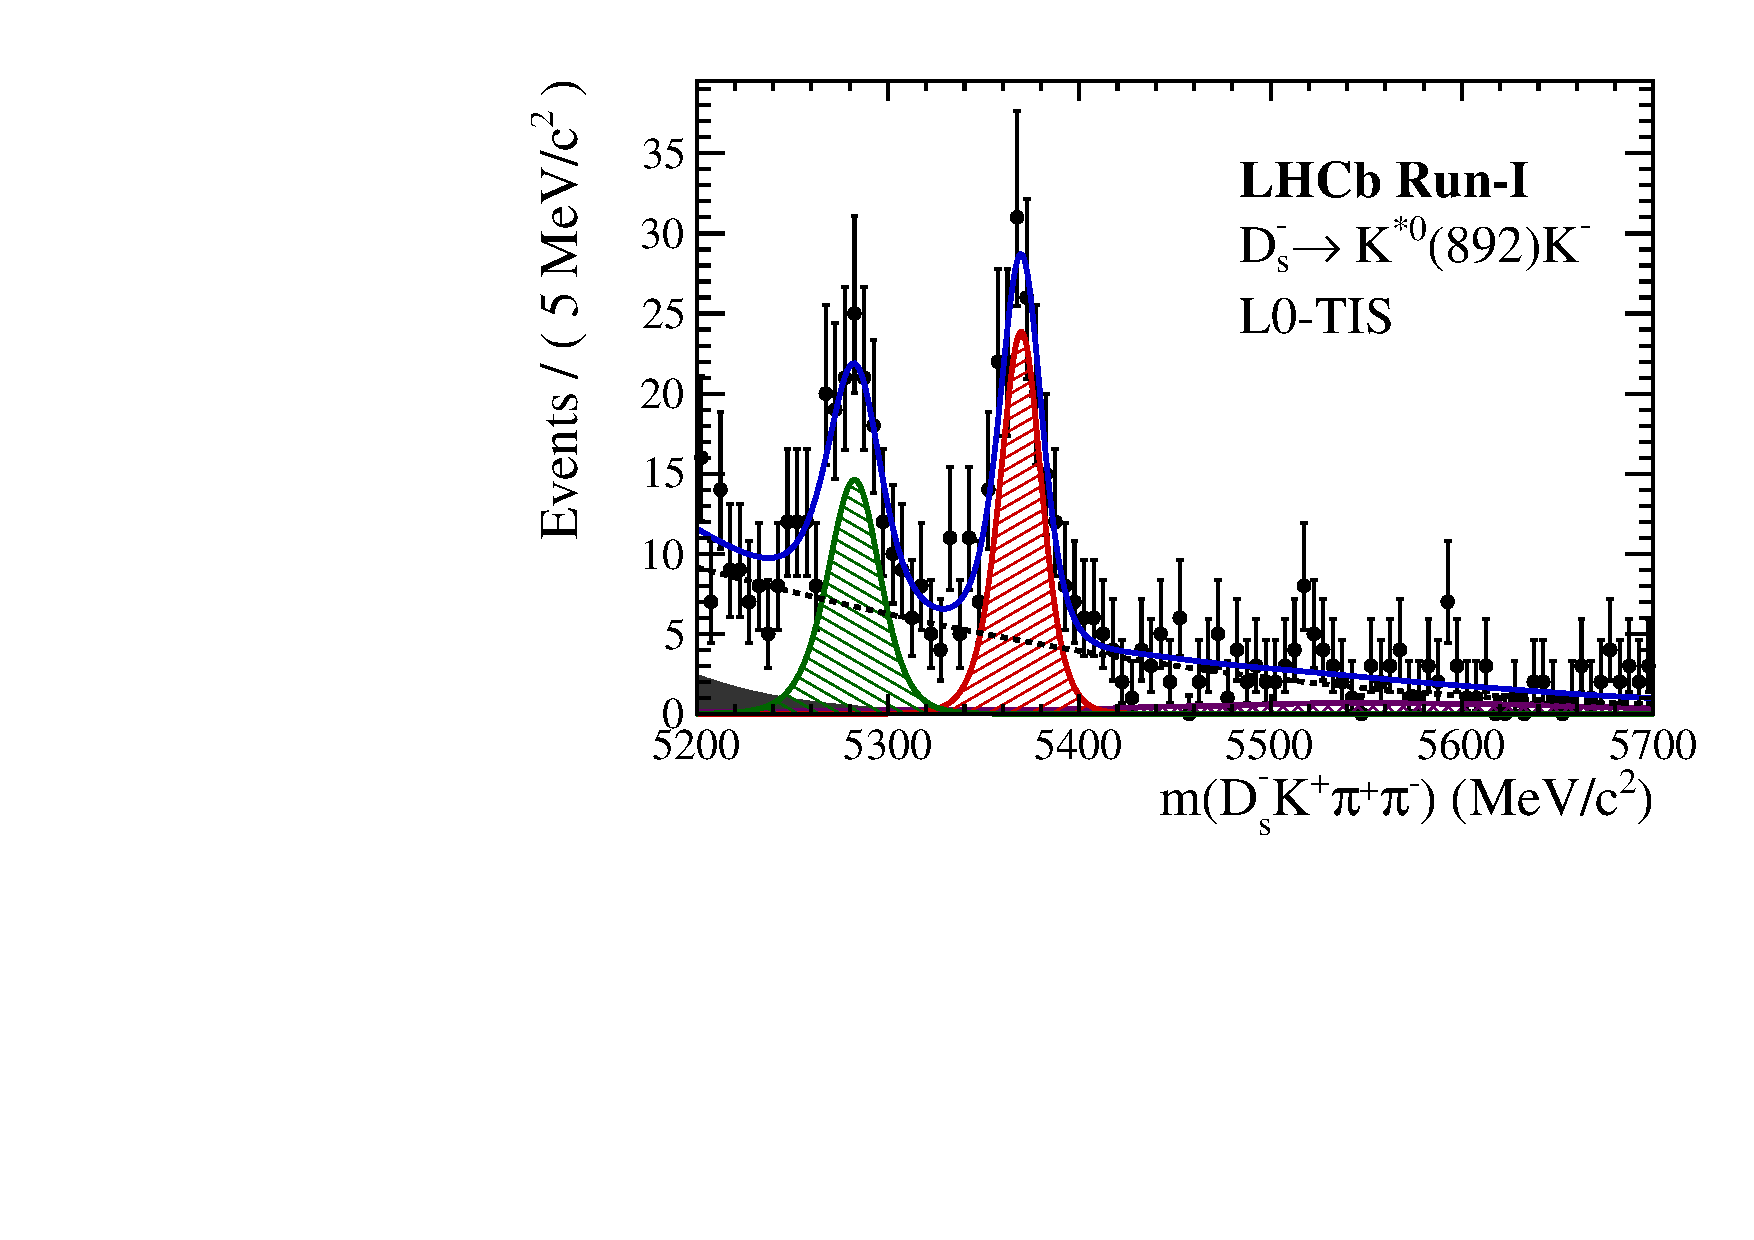
\includegraphics[height=!,width=0.4\textwidth]{figs/MassFit/signal_Run1_KsK_t1.pdf}

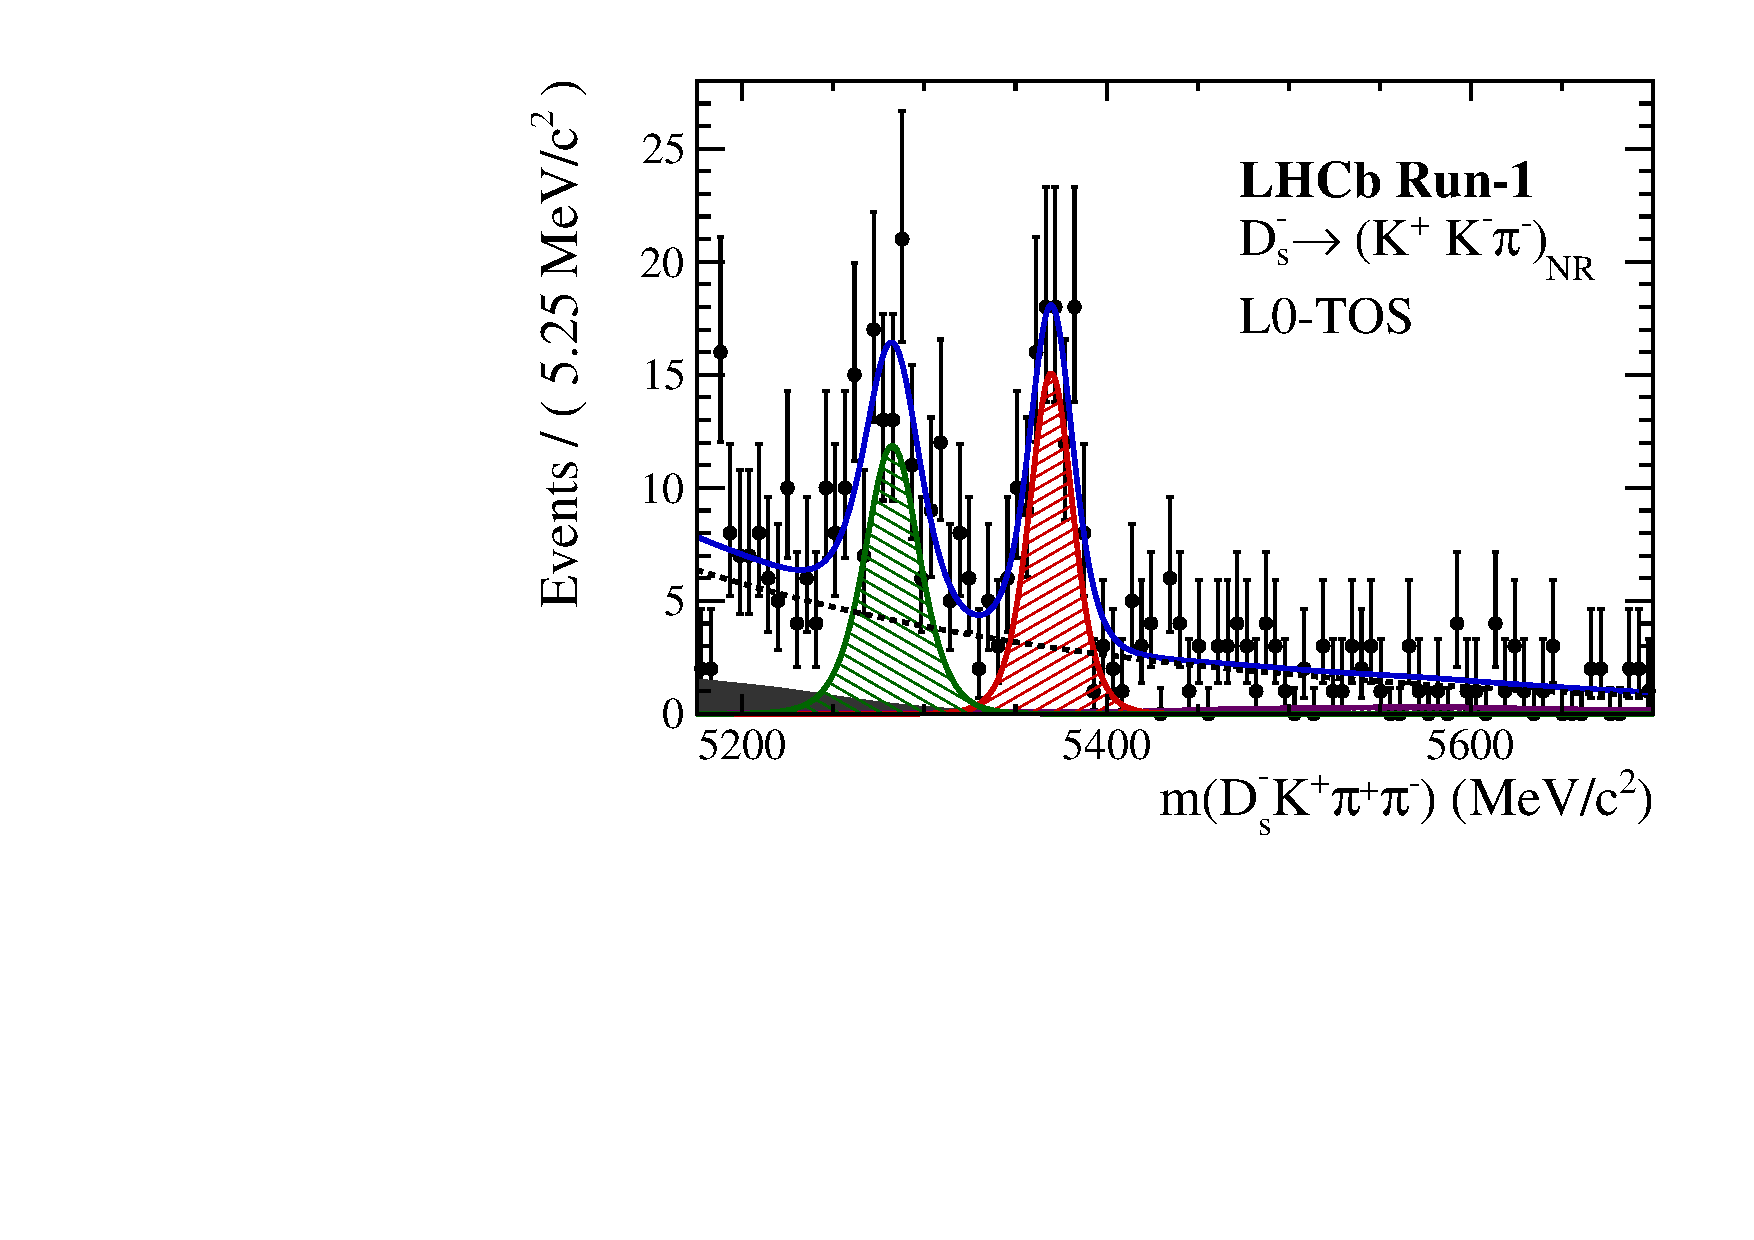
\includegraphics[height=!,width=0.4\textwidth]{figs/MassFit/signal_Run1_KKpi_NR_t0.pdf}
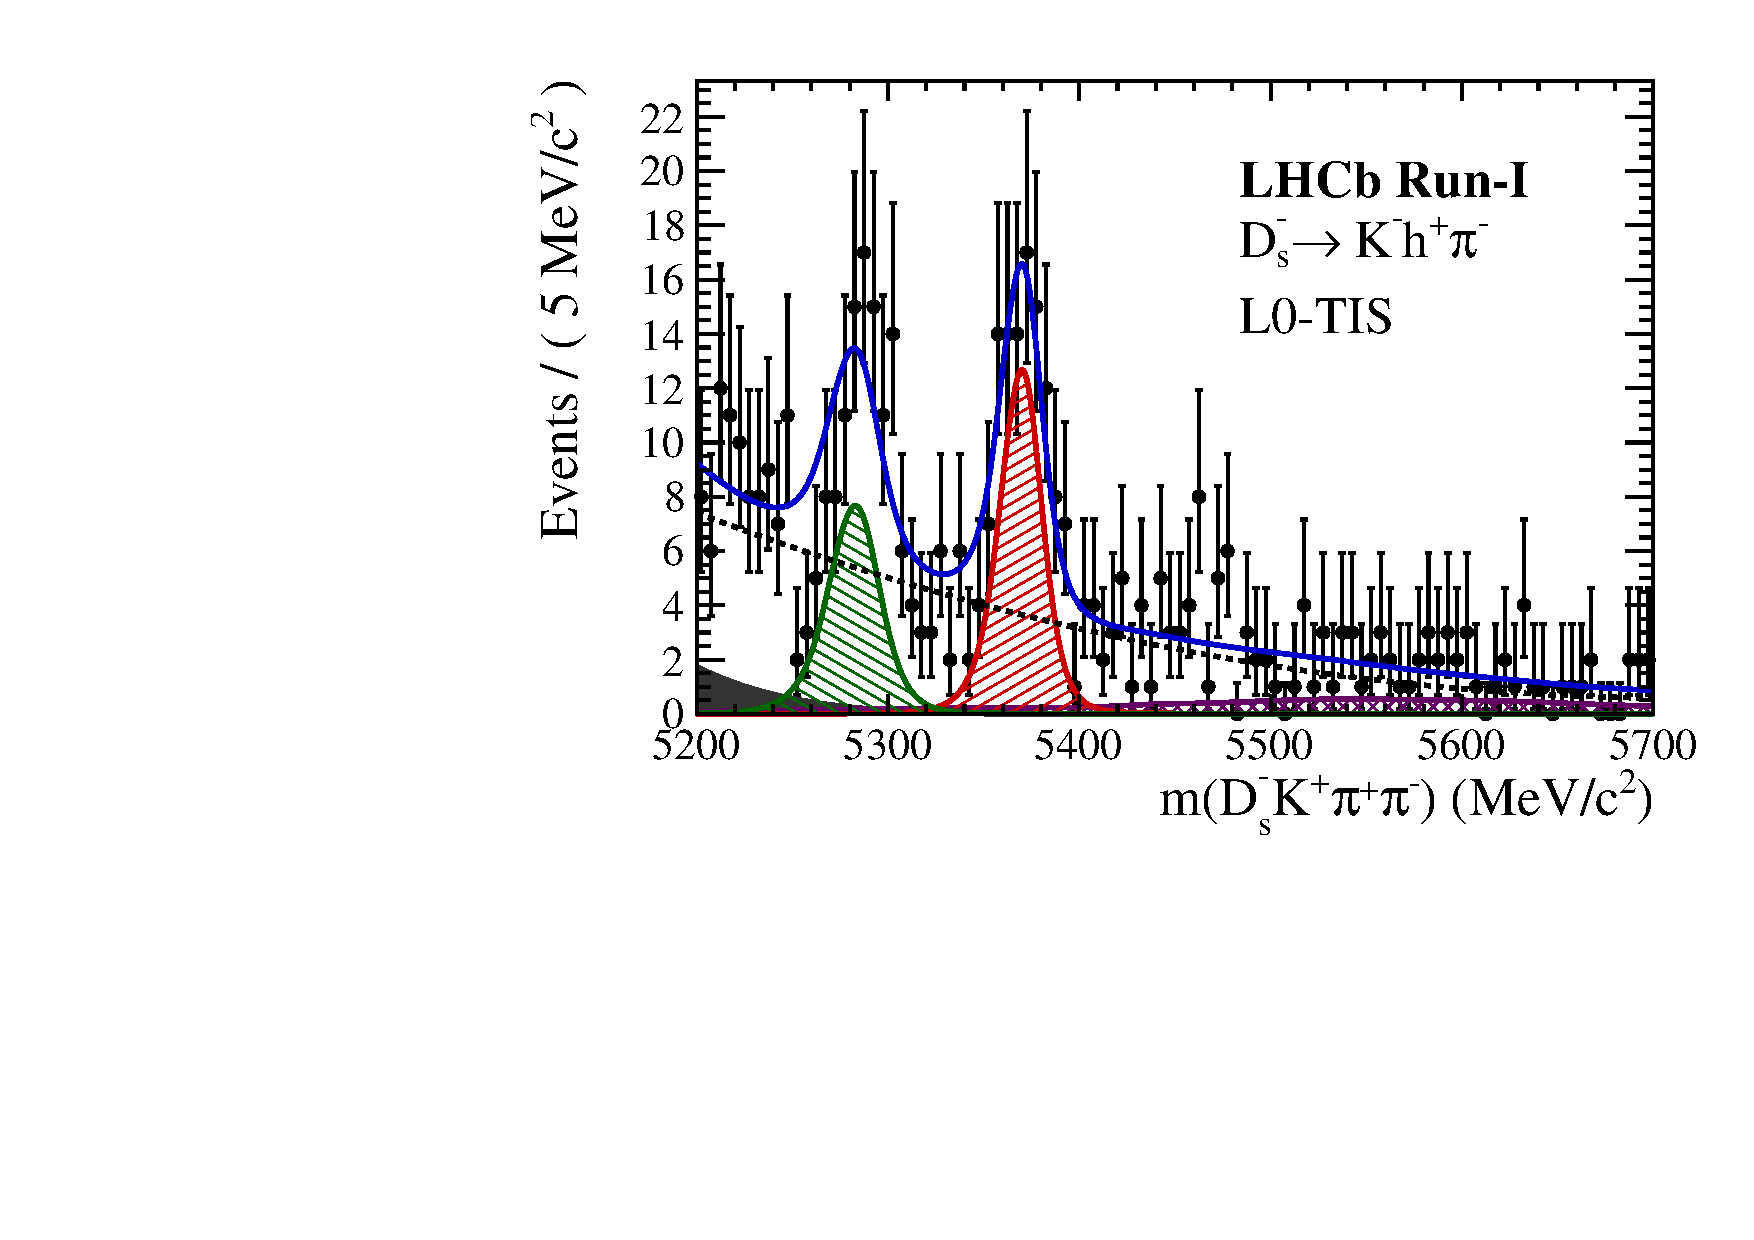
\includegraphics[height=!,width=0.4\textwidth]{figs/MassFit/signal_Run1_KKpi_NR_t1.pdf}

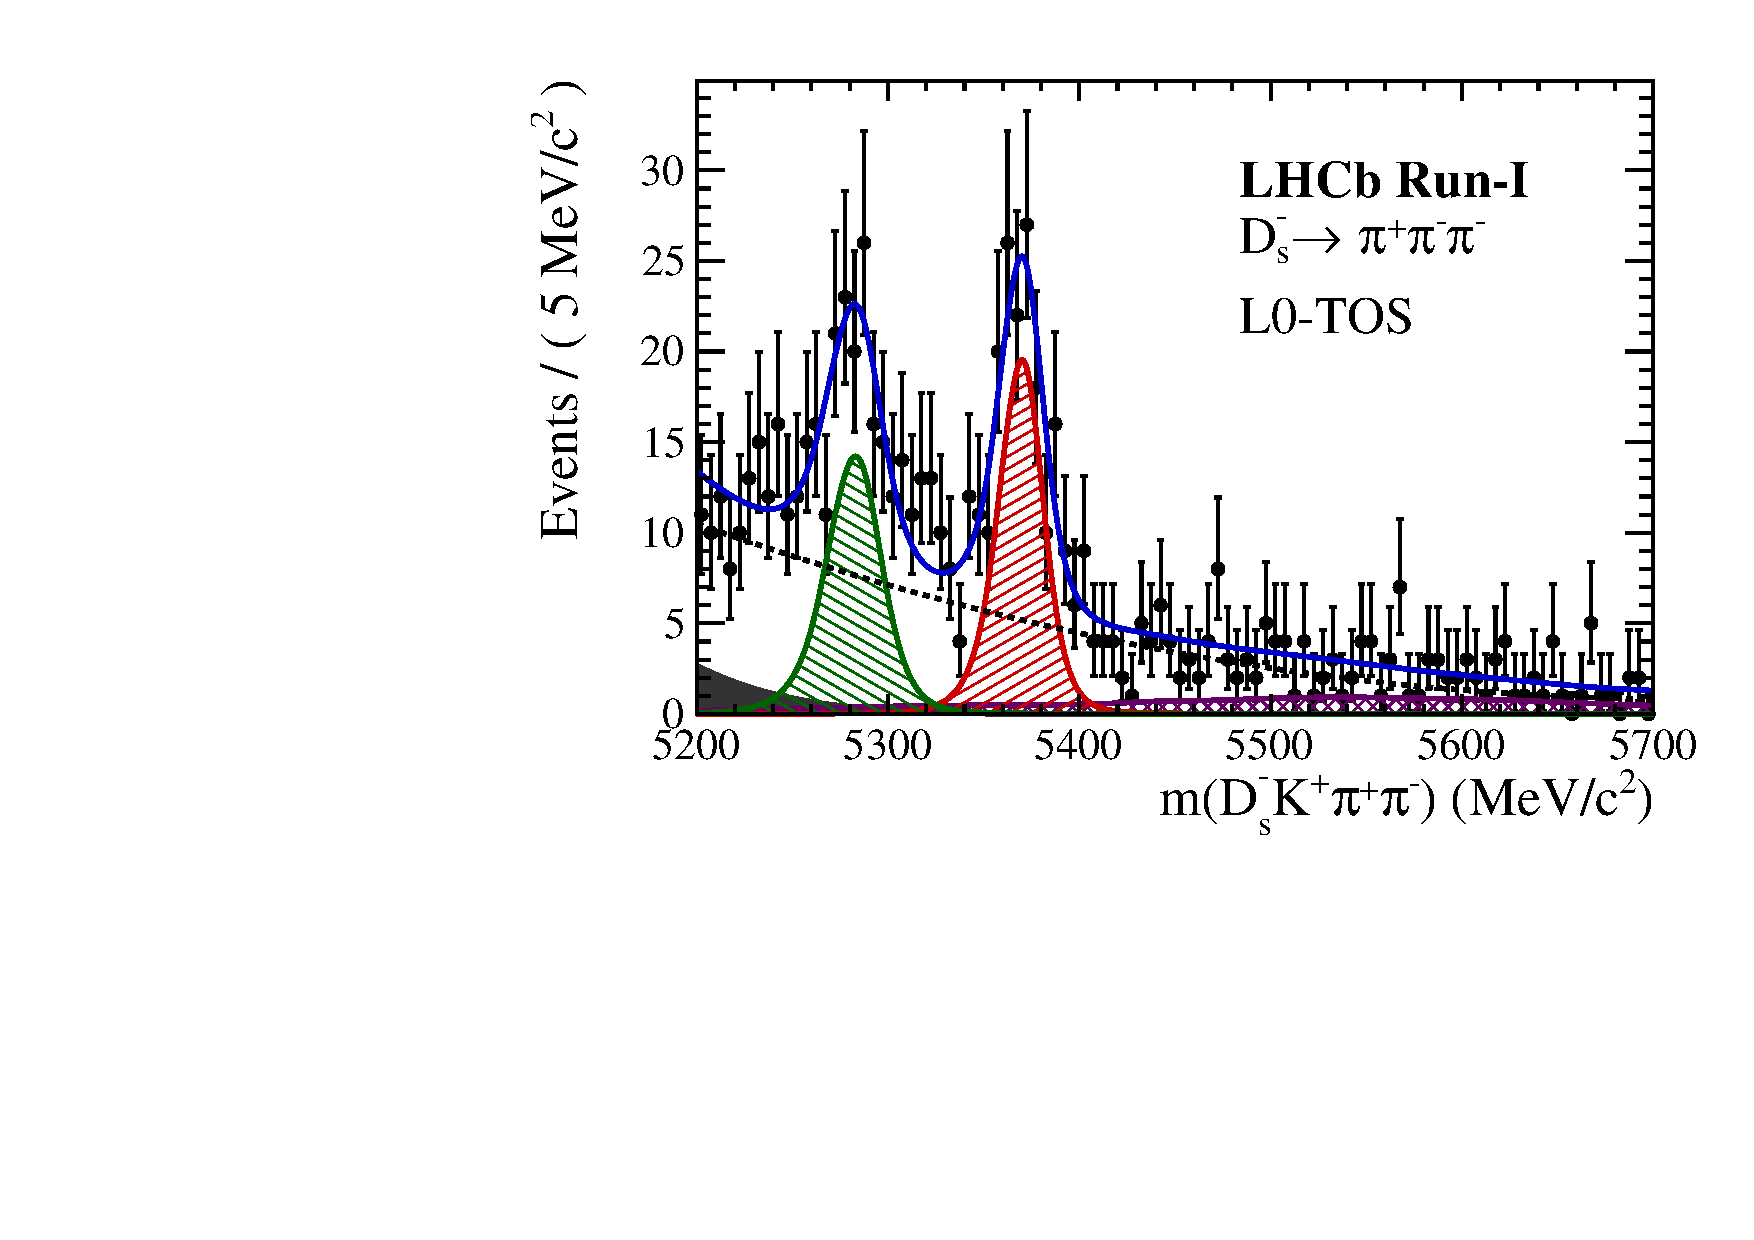
\includegraphics[height=!,width=0.4\textwidth]{figs/MassFit/signal_Run1_pipipi_t0.pdf}
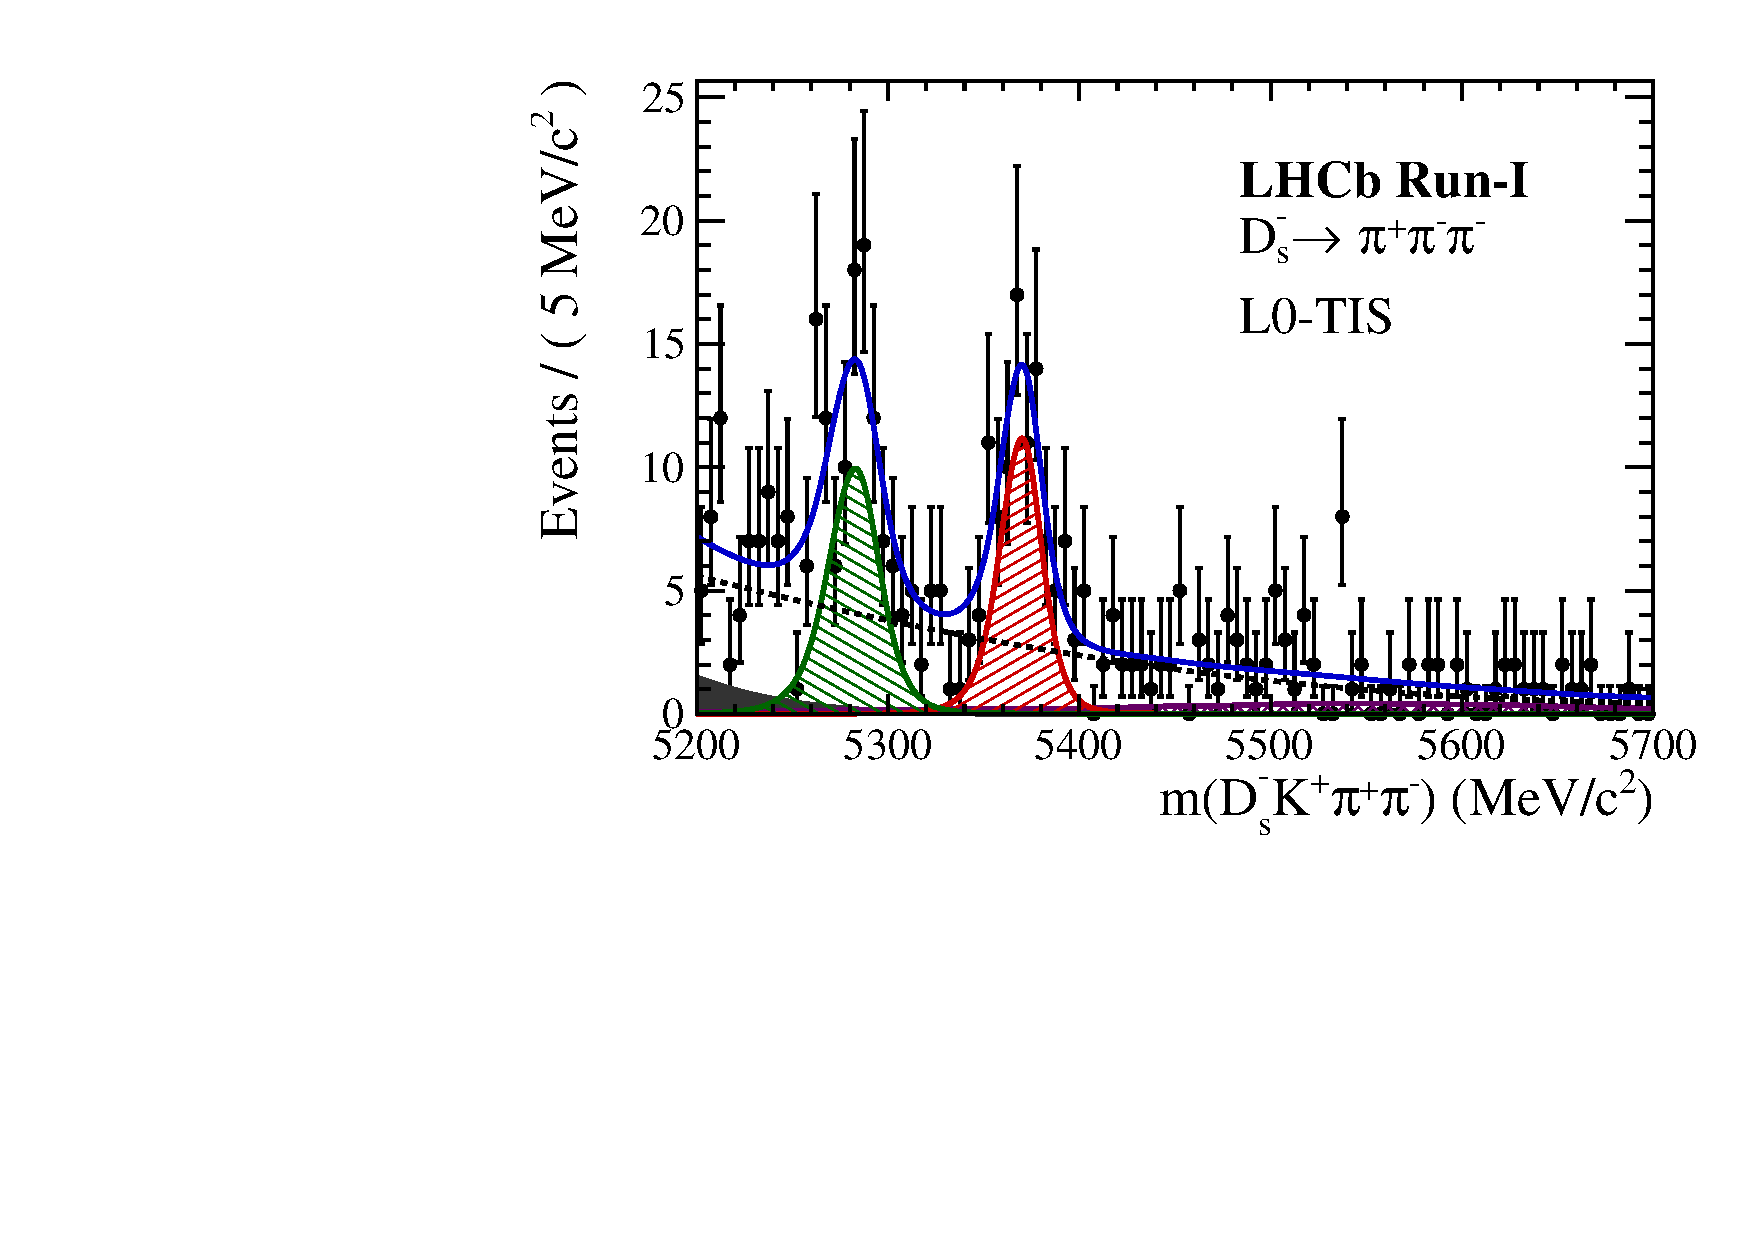
\includegraphics[height=!,width=0.4\textwidth]{figs/MassFit/signal_Run1_pipipi_t1.pdf}
\caption{Invariant mass distributions of $\Bs\to\Ds K\pion\pion$ candidates for Run-I data.}
\label{fig:massfits_signal_Run1}
\end{figure}

\clearpage

\begin{figure}[h]
\centering
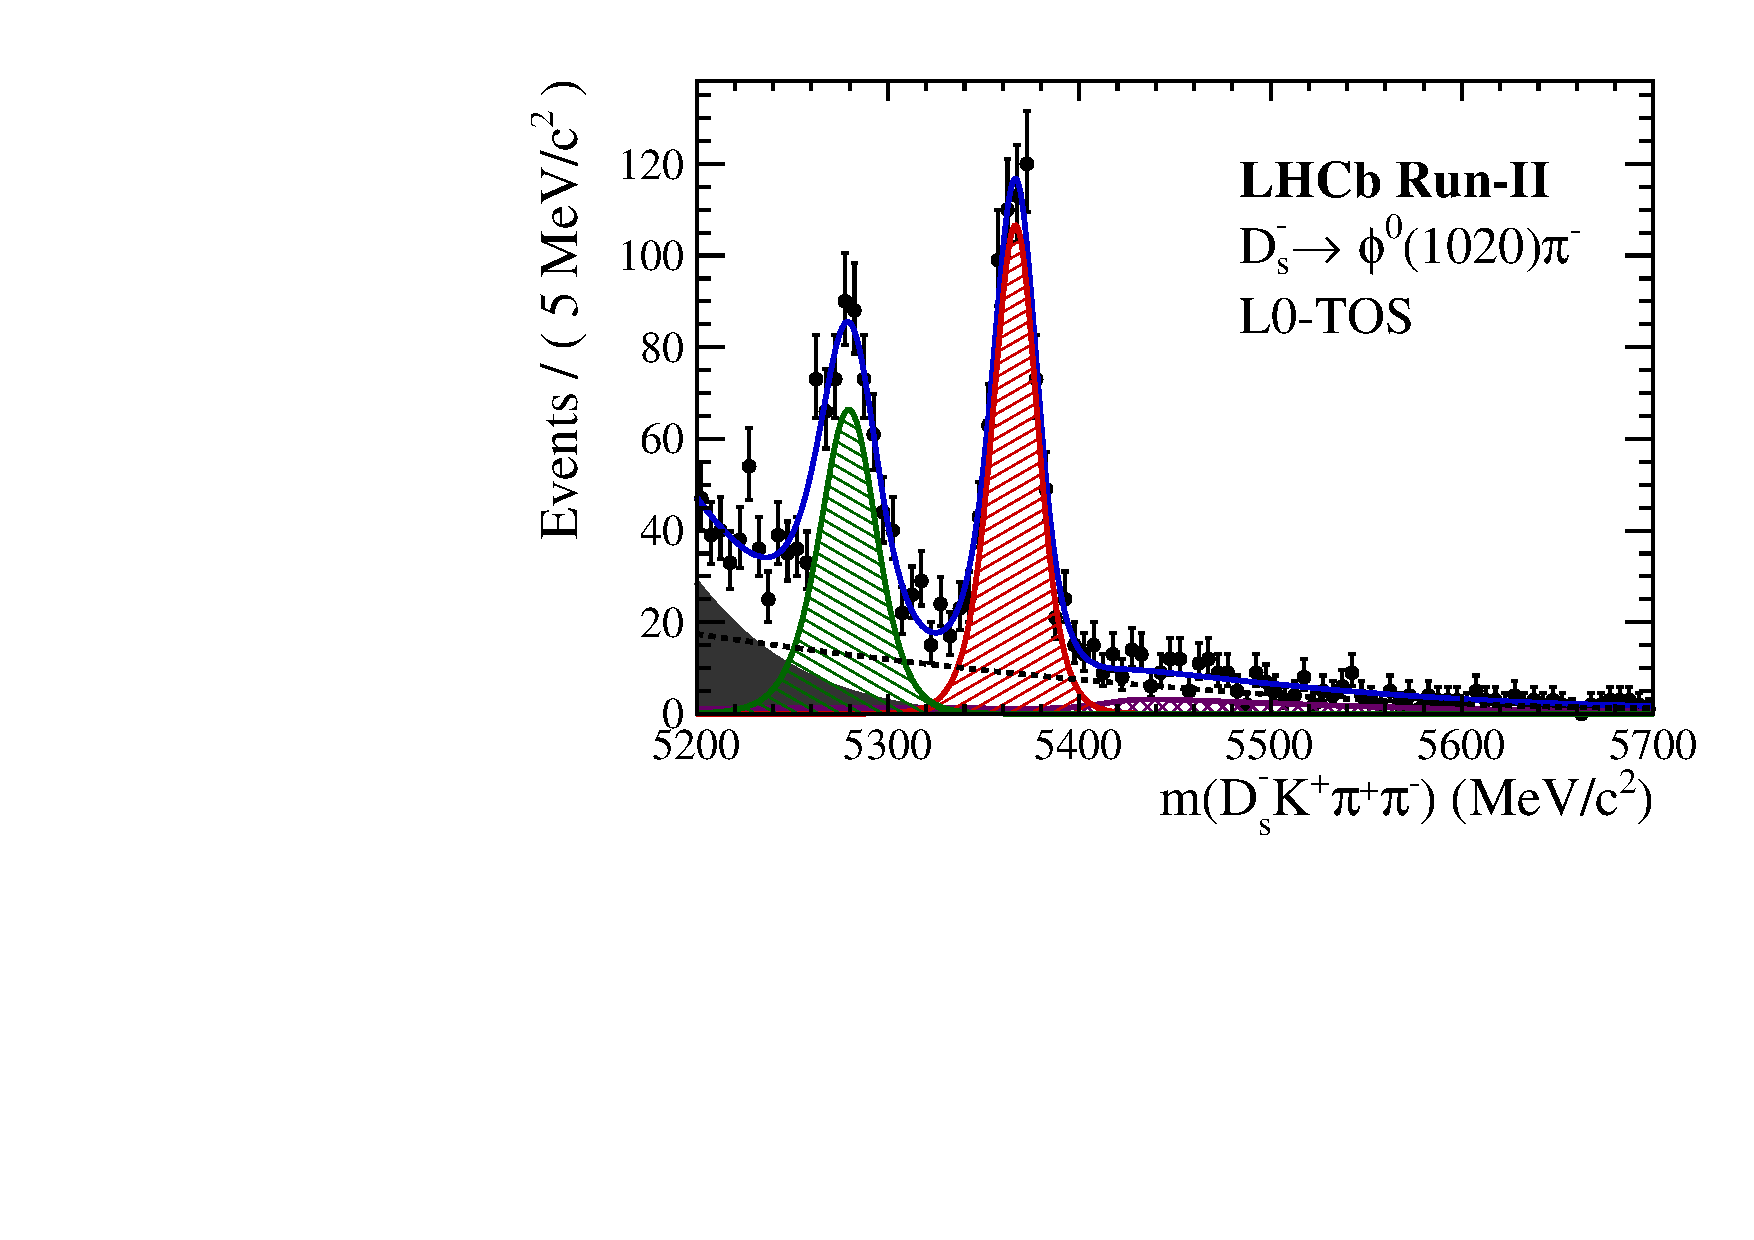
\includegraphics[height=!,width=0.4\textwidth]{figs/MassFit/signal_Run2_phipi_t0.pdf}
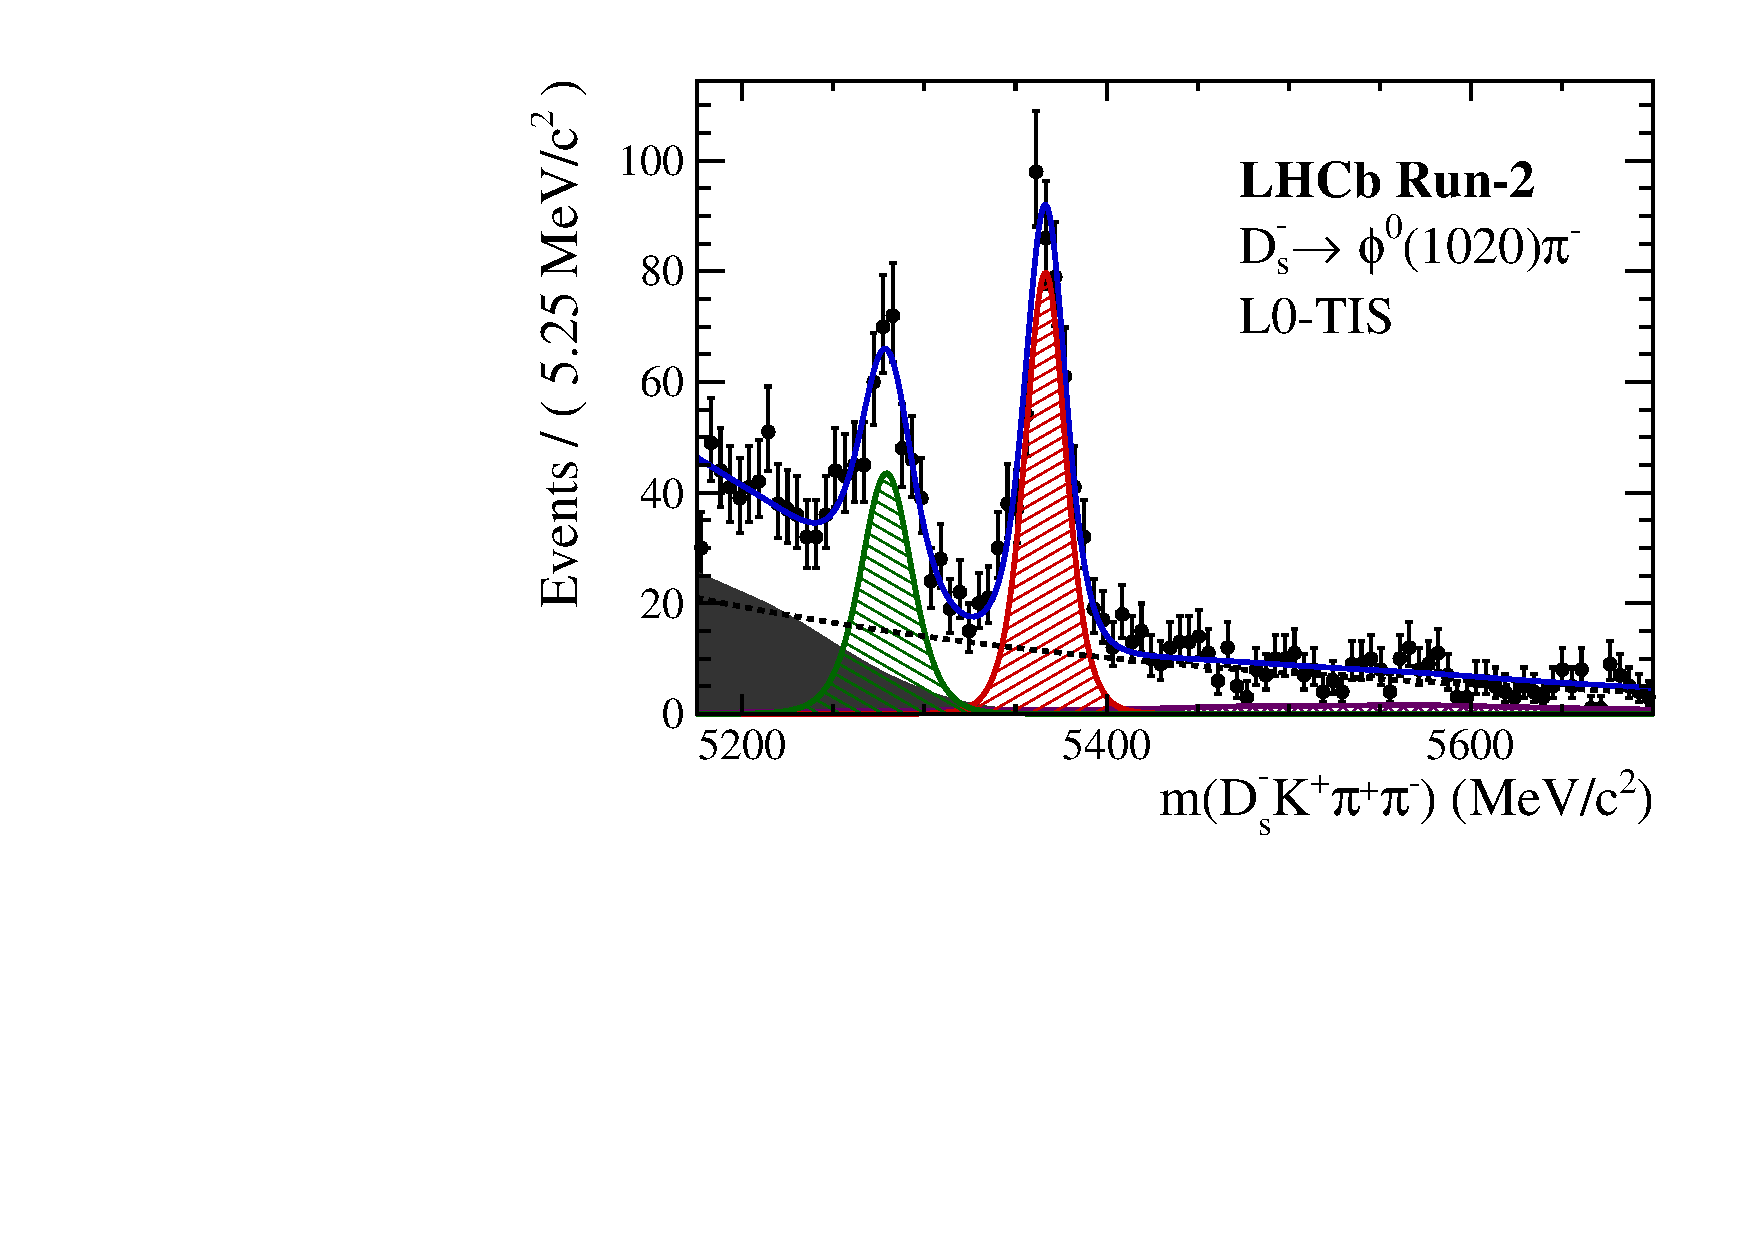
\includegraphics[height=!,width=0.4\textwidth]{figs/MassFit/signal_Run2_phipi_t1.pdf}

\includegraphics[height=!,width=0.4\textwidth]{figs/MassFit/signal_Run2_KsK_t0.pdf}
\includegraphics[height=!,width=0.4\textwidth]{figs/MassFit/signal_Run2_KsK_t1.pdf}

\includegraphics[height=!,width=0.4\textwidth]{figs/MassFit/signal_Run2_KKpi_NR_t0.pdf}
\includegraphics[height=!,width=0.4\textwidth]{figs/MassFit/signal_Run2_KKpi_NR_t1.pdf}

\includegraphics[height=!,width=0.4\textwidth]{figs/MassFit/signal_Run2_pipipi_t0.pdf}
\includegraphics[height=!,width=0.4\textwidth]{figs/MassFit/signal_Run2_pipipi_t1.pdf}

\caption{Invariant mass distributions of $\Bs\to\Ds K\pion\pion$ candidates for Run-II data.}
\label{fig:massfits_signal_Run2}
\end{figure}


\clearpage
\section{Decay-time Resolution fits}
\label{sec:DecResFits}

\setcounter{figure}{0}
\setcounter{table}{0}

\renewcommand{\thefigure}{C.\arabic{figure}}

This section contains all fits to the distributions of the decay time difference $\Delta t$ between the true and the reconstructed decay time of the truth-matched $\Bs$ candidates on MC.
The fits are performed in bins of the decay time error $\sigma_{t}$, where an adaptive binning scheme is used to ensure that approximately the same number of events are found in each bin. 

\begin{figure}[h]
\centering
\includegraphics[height=!,width=0.4\textwidth]{figs/Resolution/SignalMC_bin_1.pdf}
\includegraphics[height=!,width=0.4\textwidth]{figs/Resolution/SignalMC_bin_2.pdf}

\includegraphics[height=!,width=0.4\textwidth]{figs/Resolution/SignalMC_bin_3.pdf}
\includegraphics[height=!,width=0.4\textwidth]{figs/Resolution/SignalMC_bin_4.pdf}

\includegraphics[height=!,width=0.4\textwidth]{figs/Resolution/SignalMC_bin_5.pdf}
\includegraphics[height=!,width=0.4\textwidth]{figs/Resolution/SignalMC_bin_6.pdf}

\includegraphics[height=!,width=0.4\textwidth]{figs/Resolution/SignalMC_bin_7.pdf}
\includegraphics[height=!,width=0.4\textwidth]{figs/Resolution/SignalMC_bin_8.pdf}
\caption{Difference of the true and measured decay time of $\Bs\to\Ds\kaon\pion\pion$ MC candidates in bins of the per-event decay time error estimate..}
\label{fig:}
\end{figure}

\clearpage

\begin{figure}[h]
\centering
\includegraphics[height=!,width=0.4\textwidth]{figs/Resolution/SignalData_16_bin_1.pdf}
\includegraphics[height=!,width=0.4\textwidth]{figs/Resolution/SignalData_16_bin_2.pdf}

\includegraphics[height=!,width=0.4\textwidth]{figs/Resolution/SignalData_16_bin_3.pdf}
\includegraphics[height=!,width=0.4\textwidth]{figs/Resolution/SignalData_16_bin_4.pdf}

\includegraphics[height=!,width=0.4\textwidth]{figs/Resolution/SignalData_16_bin_5.pdf}
\includegraphics[height=!,width=0.4\textwidth]{figs/Resolution/SignalData_16_bin_6.pdf}

\includegraphics[height=!,width=0.4\textwidth]{figs/Resolution/SignalData_16_bin_7.pdf}
\includegraphics[height=!,width=0.4\textwidth]{figs/Resolution/SignalData_16_bin_8.pdf}

\includegraphics[height=!,width=0.4\textwidth]{figs/Resolution/SignalData_16_bin_9.pdf}
\includegraphics[height=!,width=0.4\textwidth]{figs/Resolution/SignalData_16_bin_10.pdf}
\caption{Decay-time distribution for fake $B_s$ candidates from promptly produced $D_s$ candidates, combined with random prompt $K\pi\pi$ bachelor tracks, for bins in the per-event decay time error estimate. Data taken in 2016.}
\label{fig:}
\end{figure}


\begin{figure}[h]
\centering
\includegraphics[height=!,width=0.4\textwidth]{figs/Resolution/SignalData_17_bin_1.pdf}
\includegraphics[height=!,width=0.4\textwidth]{figs/Resolution/SignalData_17_bin_2.pdf}

\includegraphics[height=!,width=0.4\textwidth]{figs/Resolution/SignalData_17_bin_3.pdf}
\includegraphics[height=!,width=0.4\textwidth]{figs/Resolution/SignalData_17_bin_4.pdf}

\includegraphics[height=!,width=0.4\textwidth]{figs/Resolution/SignalData_17_bin_5.pdf}
\includegraphics[height=!,width=0.4\textwidth]{figs/Resolution/SignalData_17_bin_6.pdf}

\includegraphics[height=!,width=0.4\textwidth]{figs/Resolution/SignalData_17_bin_7.pdf}
\includegraphics[height=!,width=0.4\textwidth]{figs/Resolution/SignalData_17_bin_8.pdf}

\includegraphics[height=!,width=0.4\textwidth]{figs/Resolution/SignalData_17_bin_9.pdf}
\includegraphics[height=!,width=0.4\textwidth]{figs/Resolution/SignalData_17_bin_10.pdf}

\includegraphics[height=!,width=0.4\textwidth]{figs/Resolution/SignalData_17_bin_11.pdf}
\caption{Decay-time distribution for fake $B_s$ candidates from promptly produced $D_s$ candidates, combined with random prompt $K\pi\pi$ bachelor tracks, for bins in the per-event decay time error estimate. Data taken in 2017.}
\label{fig:}
\end{figure}

\clearpage

\input{tables/Resolution/ResoTable_MC.txt}
\input{tables/Resolution/ResoTable_Data_16.txt}
\input{tables/Resolution/ResoTable_Data_17.txt}

\clearpage
\section{Comparison of time-acceptance in subsamples} 
\label{a:timeAcc}

Figure \ref{fig:AccComp} shows the spline coefficients obtained by fitting the decay-time distribution of $\Bs\to\Ds\pion\pion\pion$ data candidates
in different subsamples.
Sufficient agreement is observed within a given data-taking period, while the acceptance shapes for Run-I and Run-II data differ significantly.
The fitted splines for the different $D_s$ final states are in a good agreement.
The largest deviations are observed between the different \textsf{L0} categories.

%It is possible that the decay-time dependent efficiency deviates in different subsamples of our data 
%such as the year of data-taking, the various $\Ds$ final states or the ways an event is triggered at the \textsf{L0} stage.
%
%To investigate possible deviations, the $\Bs\to\Ds\pion\pion\pion$ sample 
%is split into subsamples according to the categories mentioned above (run, $\Ds$ state, L0 trigger). 
%For each subsample, the fit procedure described at the beginning of this chapter, using the pdf given by Eq. \ref{eq:AccPDF}, is repeated and the obtained values for the spline coefficients  $v_{i}$ are compared.
%Figure \ref{fig:AccComp} shows the comparison of the obtained spline coefficients for the different $\Ds$ final states.
%Investigating the obtained spline coefficients from different $\Ds$ final states, 
%good agreement is observed between all four channels and no need to distinguish between different final states in the time-dependent amplitude fit is found. \newline
%The comparison between spline coefficients for the different runs and L0 trigger categories is shown in Figure \ref{fig:AccCompRunTrig}.
%
%Significant deviations between spline coefficients obtained from the two different runs and L0 trigger categories can be observed. 
%The deviations are most pronounced in the $(0-5) \ps$ region, where the majority of statistics is found. 
%Therefore, the time-dependent efficiency has to be treated separately for the runs and L0 categories. 
%This is achieved by implementing a simultaneous fit, where the acceptance description is allowed to vary in the subsamples.   


\begin{figure}[h]
\centering
\includegraphics[height=!,width=0.45\textwidth]{figs/Acceptance/timeAcc_comparison_by_year_t1_adaptive_N4.pdf}
\includegraphics[height=!,width=0.45\textwidth]{figs/Acceptance/timeAcc_comparison_by_run_adaptive_N4.pdf}

\includegraphics[height=!,width=0.45\textwidth]{figs/Acceptance/timeAcc_comparison_by_DsFinalState_mod_adaptive_N4.pdf}
\includegraphics[height=!,width=0.45\textwidth]{figs/Acceptance/timeAcc_comparison_by_trigger_adaptive_N4.pdf}
\caption{Comparison of the spline coefficients (point with error bars) obtained from time-dependent fits to the $\Bs\to\Ds\pion\pion\pion$ decay-time for different subsamples:
(top-left) different years of data-taking; (top-right) different data-taking periods;
(bottom-left) different $D_s$ final states; (bottom-right) different trigger categories. 
The interpolated splines are overlaid.}
\label{fig:AccComp}
\end{figure}

\clearpage
\section{Spin Amplitudes} 
\label{a:sf}

The spin factors used for $B \to P_1 \, P_2 \, P_3 \, P_4$ decays are given in Table \ref{tab:Sf}.
%\renewcommand{\thetable}{B.\arabic{table}}

\begin{table}[h]
  \scriptsize
  \centering
  \caption{\small Spin factors for all topologies considered in this analysis. 
  In the decay chains, $S$, $P$, $V$, $A$, $T$ and $PT$ stand for scalar, pseudoscalar, vector, axial vector, tensor and pseudotensor, respectively. 
  If no angular momentum is specified, the lowest angular momentum state compatible with angular momentum conservation and, where appropriate, parity conservation, is used.}
  	\resizebox{\linewidth}{!}{
	\begin{tabular}{@{\hspace{0.5cm}}c@{\hspace{0.25cm}} @{\hspace{0.25cm}} l@{\hspace{0.25cm}}  @{\hspace{0.25cm}}l@{\hspace{0.5cm}}}
     \hline \hline
	Number & Decay chain & Spin amplitude  \\ \hline
	1 & $B \to (P \, P_{1})$, $P \to (S \, P_{2})$, $S \to (P_{3} \, P_{4})$ & $1$ \\
	 2 & $B \to (P \, P_{1})$, $P \to (V \, P_{2})$, $V \to (P_{3} \, P_{4})$ & $L_{(1)\alpha}(P) \,   \, L_{(1)}^{\alpha}(V) $ \\

	 3 & $B \to (A \, P_{1})$, $A \to (V \, P_{2})$, $V \to (P_{3} \, P_{4})$ & $L_{(1)\alpha}(B) \, P_{(1)}^{\alpha \beta}(A)  \, L_{(1)\beta}(V) $ \\
	 4 & $B \to (A \, P_{1})$, $A[D] \to (P_{2} \, V)$, $V \to (P_{3} \, P_{4})$ & $L_{(1)\alpha}(B) \, L_{(2)}^{\alpha \beta}(A)  \, L_{(1)\beta}(V) $   \\
	 5 & $B \to (A \, P_{1})$, $A \to (S \, P_{2})$, $S \to (P_{3} \, P_{4})$ & $L_{(1)\alpha}(B) \, L_{(1)}^{\alpha}(A) $    \\
	6 &  $B \to (A \, P_{1})$, $A \to (T \, P_{2})$, $T \to (P_{3} \, P_{4})$ &  $L_{(1)\alpha}(B) \, L_{(1)\beta}(A) \, L_{(2)}^{\alpha \beta}(T) $  \\
	
	7 &  $B \to (V_{1} \, P_{1})$, $V_{1} \to (V_{2} \, P_{2})$, $V_{2} \to (P_{3} \, P_{4})$ & 
	$ L_{(1)\mu}(B) \, P_{(1)}^{\mu \alpha }(V_{1})  \, \epsilon_{\alpha \beta \gamma \delta} \, L_{(1)}^{\beta}(V_{1}) \, p_{V_{1}}^{\gamma} \, L_{(1)}^{\delta}(V_{2}) $ \\
	
	 8 & $B \to (PT \, P_{1})$, $PT \to (V \, P_{2})$, $V \to (P_{3} \, P_{4})$ & 
	  $L_{(2)\alpha \beta}(B) \, P_{(2)}^{\alpha \beta \gamma \delta}(PT)  \, L_{(1)\gamma}(PT) \, L_{(1)\delta}(V) $ \\
	 9 &  $B \to (PT \, P_{1})$, $PT \to (S \, P_{2})$, $S \to (P_{3} \, P_{4})$ & 
	  $L_{(2)\alpha \beta}(B)  \, L_{(2)}(PT)^{\alpha \beta}  $ \\
	  10 & $B \to (PT \, P_{1})$, $PT \to (T \, P_{2})$, $T \to (P_{3} \, P_{4})$ & 
	  $L_{(2)\alpha \beta}(B) \, P_{(2)}^{\alpha \beta \gamma \delta}(PT)  \, L_{(2)\gamma \delta}(T)  $ \\
	  
	   11 & $B \to (T \, P_{1})$, $T \to (V \, P_{2})$, $V \to (P_{3} \, P_{4})$ & 
	  $L_{(2)\mu \nu}(B) \, P_{(2)}^{\mu \nu \rho \alpha}(T)  \, \epsilon_{\alpha \beta \gamma \delta}  
	  \, L_{(2)\rho}^{\beta}(T) \, p_{T}^{\gamma} \,  P_{(1)}^{\delta \sigma}(T) \, L_{(1)\sigma}(V) $ \\
	  
	   12 & $B \to (T_{1} \, P_{1})$, $T_{1} \to (T_{2} \, P_{2})$, $T_{2} \to (P_{3} \, P_{4})$ & 
	  $L_{(2)\mu \nu}(B) \, P_{(2)}^{\mu \nu \rho \alpha}(T_{1})  \, \epsilon_{\alpha \beta \gamma \delta}  
	  \, L_{(1)}^{\beta}(T_{1}) \, p_{T_{1}}^{\gamma} \,  L_{(2)\rho}^{\delta}(T_{2}) $ \\

	  13 & $B \to (S_{1} \, S_{2})$, $S_{1} \to (P_{1} \, P_{2})$, $S_{2} \to (P_{3} \, P_{4})$ & $ 1$ \\	  
	 
	  14 & $B \to (V \, S)$, $V \to (P_{1} \, P_{2})$, $S \to (P_{3} \, P_{4})$ & $L_{(1)\alpha}(B) \, L_{(1)}^{\alpha}(V) $ \\
	 
	  15 & $B \to (V_{1} \, V_{2})$, $V_{1} \to (P_{1} \, P_{2})$, $V_{2} \to (P_{3} \, P_{4})$ & $L_{(1)\alpha}(V_{1})  \, L_{(1)}^{\alpha}(V_{2}) $ \\
	  16 & $B[P] \to (V_{1} \, V_{2})$, $V_{1} \to (P_{1} \, P_{2})$, $V_{2} \to (P_{3} \, P_{4})$ & 
	 $\epsilon_{\alpha \beta \gamma \delta} \, L_{(1)}^{\alpha}(B) \, L_{(1)}^{\beta}(V_{1}) \, L_{(1)}^{\gamma}(V_{2}) \, p_{B}^{\delta}$ \\
	 17 &  $B[D] \to (V_{1} \, V_{2})$, $V_{1} \to (P_{1} \, P_{2})$, $V_{2} \to (P_{3} \, P_{4})$ &   $ L_{(2)\alpha \beta}(B)  \,L_{(1)}^{\alpha}(V_{1}) \, L_{(1)}^{\beta}(V_{2}) $ \\

	   18 & $B \to (T \, S)$, $T \to (P_{1} \, P_{2})$, $S \to (P_{3} \, P_{4})$ & $L_{(2)\alpha \beta}(B) \, L_{(2)}^{\alpha \beta}(T) $ \\
	   19 & $B \to (V \, T)$, $T \to (P_{1} \, P_{2})$, $V \to (P_{3} \, P_{4})$ & $L_{(1)\alpha}(B) \, L_{(2)}^{\alpha \beta}(T) \, L_{(1)\beta}(V) $ \\
	   20 & $B[D] \to (T \, V)$, $T \to (P_{1} \, P_{2})$, $V \to (P_{3} \, P_{4})$ &
	   $\epsilon_{\alpha \beta \delta \gamma} \, L_{2}^{\alpha \mu}(B) \, L_{2\mu}^{\beta} \, L_{(1)}^{\gamma}(V) \, p_{B}^{\delta} $ \\
	
	   21 & $B \to (T_{1} \, T_{2})$, $T_{1} \to (P_{1} \, P_{2})$, $T_{2} \to (P_{3} \, P_{4})$ & $L_{(2)\alpha \beta}(T_{1}) \, L_{(2)}^{\alpha \beta}(T_{2}) $ \\
	  22 &  $B[P] \to (T_{1} \, T_{2})$, $T_{1} \to (P_{1} \, P_{2})$, $T_{2} \to (P_{3} \, P_{4})$ & 
	  $\epsilon_{\alpha \beta \gamma \delta} \, L_{(1)}^{\alpha}(B) \, L_{(2)}^{\beta \mu}(T_{1}) \, L_{(2)\mu}^{\gamma}(T_{2}) \, p_{B}^{\delta} $ \\
	  23 &  $B[D] \to (T_{1} \, T_{2})$, $T_{1} \to (P_{1} \, P_{2})$, $T_{2} \to (P_{3} \, P_{4})$ & 
	  $L_{(2)\alpha \beta}(B) \, L_{(2)}^{\alpha \gamma}(T_{1}) \, L_{(2)\gamma}^{\beta}(T_{2}) $ \\

     \hline \hline
	\end{tabular}
	}
	\label{tab:Sf}
\end{table}



\clearpage\section{Considered Decay Chains}
\label{a:decays}

The various decay channels considered in the model building are listed in Table \ref{tab:components}.
%\setcounter{table}{0}
%\renewcommand{\thetable}{C.\arabic{table}}

\begin{table}[h]
  \small
  \centering
  \caption{Decays considered in the LASSO model building. \label{tab:components}}
           \begin{tabular} {@{\hspace{0.5cm}}l@{\hspace{0.25cm}}}
     \hline \hline
	 Decay channel  \\ \hline
              %cascade 
              $B_s \to D_s^- \, [K_{1}(1270)^{+}[S,D]\to \pi^+ \, K^{*}(892)^{0}]$ \\
              $B_s \to D_s^- \, [K_{1}(1270)^{+}\to \pi^+ \, K^{*}(1430)^{0}]$ \\
              $B_s \to D_s^- \, [K_{1}(1270)^{+}[S,D]\to K^+ \, \rho(770)^{0}]$ \\
              $B_s \to D_s^- \, [K_{1}(1270)^{+}[S,D]\to K^+ \, \omega(782)]$ \\
              $B_s \to D_s^- \, [K_{1}(1400)^{+}[S,D]\to \pi^+ \, K^{*}(892)^{0}]$ \\
              $B_s \to D_s^- \, [K_{1}(1400)^{+}[S,D]\to K^+ \, \rho(770)^{0}]$ \\
              $B_s \to D_s^- \, [K(1460)^{+}\to \pi^+ \, \kappa]$ \\
              $B_s \to D_s^- \, [K(1460)^{+}\to K^+ \, \sigma]$ \\
              $B_s \to D_s^- \, [K(1460)^{+}\to \pi^+ \, K^{*}(892)^{0}]$ \\
              $B_s \to D_s^- \, [K(1460)^{+}\to K^+ \, \rho(770)^{0}]$ \\
              $B_s \to D_s^- \, [K^{*}(1410)^+\to \pi^+\, K^{*}(892)^{0}]$ \\
              $B_s \to D_s^- \, [K^{*}(1410)^+\to K^+ \, \rho(770)^{0}]$ \\
              $B_s \to D_s^- \, [K_{2}^*(1430)^{+}\to \pi^+ \, K^{*}(892)^{0}]$ \\
              $B_s \to D_s^- \, [K_{2}^*(1430)^{+}\to K^+ \, \rho(770)^{0}]$ \\
              $B_s \to D_s^- \, [K^*(1680)^{+}\to \pi^+ \, K^{*}(892)^{0}]$ \\
              $B_s \to D_s^- \, [K^*(1680)^{+}\to K^+ \, \rho(770)^{0}]$ \\      
               $B_s \to D_s^- \, [K_{2}(1770)^{+}\to \pi^+ \, K^{*}(892)^{0}]$ \\
              $B_s \to D_s^- \, [K_{2}(1770)^{+}\to K^+ \, \rho(770)^{0}]$ \\
%              %Single res. 
              $B_s \to \sigma^{0} (D_s^- K^+)_S$ \\
              $B_s[S,P,D] \to \sigma^{0} (D_s^- K^+)_V$ \\
              $B_s \to \rho(770)^{0} (D_s^- K^+)_S$ \\
              $B_s[S,P,D] \to \rho(770)^{0} \, (D_s^- K^+)_V$\\
              $B_s \to  K^{*}(892)^{0} \, (D_s^- \pi^+)_S$ \\
              $B_s[S,P,D]  \to  K^{*}(892)^{0} \, (D_s^- \pi^+)_V$ \\
              %NonResNonRes
              $B_s \to (D_s^- K^+)_{S} \, (\pi^+ \pi^-)_{S}$ \\
              \hline \hline
           \end{tabular}
\end{table}


